\PassOptionsToPackage{obeyspaces}{url}
\documentclass[oneside,final]{hcmut-report}
\usepackage{array,longtable,tabularx,enumitem,float,needspace}
\usepackage{etoolbox,seqsplit}
\usepackage{pdflscape}
% Backport the LaTeX maintainers' finite-glue fix for longtable v4.24.
% https://www.latex-project.org/news/latex2e-news/ltnews43.pdf
\makeatletter
\ifpatchable{\LT@output}{\copy\LT@foot\vss}{%
  \patchcmd{\LT@output}{\copy\LT@foot\vss}
    {\copy\LT@foot\vskip 0pt plus \maxdimen minus \normalbaselineskip}
    {}{\PackageError{genailms-report}{Cannot patch longtable output glue}{}}
  \patchcmd{\LT@output}{\copy\LT@foot\vss}
    {\copy\LT@foot\vskip 0pt plus \maxdimen minus \normalbaselineskip}
    {}{\PackageError{genailms-report}{Cannot patch second longtable output glue}{}}
}{}
\makeatother

\usepackage{url}
\makeatletter
\def\UrlBreaks{\do\/\do\_}
\makeatother
\usepackage{xcolor}
\newcolumntype{Y}{>{\raggedright\arraybackslash}X}
\newcommand{\code}[1]{{\small\nolinkurl{#1}}}
\newcommand{\hashcode}[1]{{\scriptsize\ttfamily\seqsplit{#1}}}
\newcommand{\diagram}[3]{\par\begin{figure}[H]\centering\includegraphics[width=\linewidth,height=.72\textheight,keepaspectratio]{diagrams/#1.pdf}\caption{#2}\label{fig:#3}\end{figure}\par}
\newcommand{\screen}[3]{\par\begin{figure}[H]\centering\includegraphics[width=\linewidth,height=.405\textheight,keepaspectratio]{graphics/ui/#1}\caption{#2}\label{fig:ui-#3}\end{figure}\par}
\setcounter{tocdepth}{2}
\coursename{Specialized Project}
\reporttype{Final Report (Progress Draft)}
\title{Generative AI-Based Automatic Microlearning Module Generation for LMS}
\advisor{& TS. Nguyễn Quang Hùng & \\ & PGS. TS. Thoại Nam &}
\stuname{& Dương Nguyễn Tấn Đạt & 2352222}
\reportplace{Ho Chi Minh City}
\reporttime{November 2026}
\hypersetup{pdftitle={Generative AI-Based Automatic Microlearning Module Generation for LMS - Final Report, Progress Draft - HK261-DAGD1-033},pdfauthor={Dương Nguyễn Tấn Đạt},citecolor=black,urlcolor=blue!50!black}
\setlength{\emergencystretch}{2em}
\begin{document}
\hypersetup{pageanchor=false}
\coverpage
\pagenumbering{roman}
\hypersetup{pageanchor=true}
\pagestyle{plain}
\thispagestyle{plain}
\section*{Declaration of Authenticity}
I declare that I solely conducted this Specialized Project, under the supervision of Dr. Nguyễn Quang Hùng and Assoc. Prof. Dr. Thoại Nam at the Faculty of Computer Science and Engineering, Vietnam National University -- Ho Chi Minh City University of Technology. I have taken care to properly acknowledge and document all external sources and references used in the project. If there is any instance of plagiarism, I am ready to accept the consequences. Ho Chi Minh City University of Technology -- Vietnam National University HCMC will not be held responsible for any copyright violations that may have occurred during my research.

\vspace{2\baselineskip}
\begin{flushright}
Dương Nguyễn Tấn Đạt\\
Student ID: 2352222
\end{flushright}
\clearpage
\thispagestyle{plain}
\section*{Acknowledgement}
I would like to thank my advisors, Dr. Nguyễn Quang Hùng and Assoc. Prof. Dr. Thoại Nam, for their guidance during this Specialized Project. I also express my appreciation to the Faculty of Computer Science and Engineering at Ho Chi Minh City University of Technology.
\clearpage
\section*{Abstract}
\addcontentsline{toc}{section}{Abstract}
GENAILMS (Generative Artificial Intelligence for Learning Management Systems) helps instructors turn course material into short, coherent learning modules. A module contains a learning objective, Content, Slides, Example, Practice, Quiz and Explanation, generated from passages retrieved from the instructor's own documents, with inline citations to the exact source passages. Modules are reviewed and edited in the tool and published to Moodle as Book and Quiz activities. This progress draft of the final report describes the system as implemented by November 2026 and the measurements made so far.

The system is a modular monolith of stateless services: an API that also streams course chat, a job worker for ingestion and generation, a model gateway, and a self-hosted embedder. PostgreSQL with pgvector holds data, vectors and the job queue. A Terraform description deploys it to AWS on ECS Fargate, RDS, S3, ElastiCache and CloudFront, designed to be created and destroyed per session to fit a \$200 credit. Instructors can open the tool from Moodle with an LTI 1.3 launch.

On 250 questions over five subjects, hybrid retrieval with Jina reranking reached Hit Rate@1 0.856, MRR@10 0.918 and nDCG@10 0.938. Load tests on one machine identified CPU reranking as the shared bottleneck: chat stayed at 22.5 messages per minute regardless of API tasks. A hosted reranker removed it, reaching 462 messages per minute with four API tasks and up to 638 modules per hour in short bursts, and ranked at least as well on held-out questions; on Vietnamese questions over English material its MRR was higher, though equivalent recall there is not yet demonstrated. Retrying rate-limited model calls individually raised completed modules from 1 to 30 of 32 under real provider limits.

The quality evaluation of generated modules, the sustained and failure tests, and all measurements on AWS remain. They are ready to run and wait on model credit, cloud credit and recruited raters.

\noindent\textbf{Keywords:} microlearning; generative artificial intelligence; retrieval-augmented generation; Moodle; LTI; source citations; cloud-native architecture; scalability.
\clearpage
\tableofcontents
\listoffigures
\listoftables
\clearpage
\section*{List of Abbreviations}
\addcontentsline{toc}{section}{List of Abbreviations}
\begingroup\small
\begin{longtable}{|p{3.0cm}|p{11.7cm}|}\hline
Abbreviation & Meaning\\\hline\endfirsthead
\hline Abbreviation & Meaning\\\hline\endhead
AI / GENAILMS & Artificial intelligence / Generative Artificial Intelligence for Learning Management Systems\\\hline
LMS / LLM / RAG / LO & Learning management system / large language model / retrieval-augmented generation / learning objective\\\hline
API / HTTP / HTTPS & Application programming interface / Hypertext Transfer Protocol / HTTP protected by transport encryption\\\hline
UML / ERD / RLS & Unified Modeling Language / entity--relationship diagram / row-level security\\\hline
MRR / BM25 / RRF & Mean reciprocal rank / Best Matching 25 / Reciprocal Rank Fusion\\\hline
OCR / CPU / INT8 & Optical character recognition / central processing unit / 8-bit integer weights\\\hline
JWT / UUID / PK / FK & JSON Web Token / universally unique identifier / primary key / foreign key\\\hline
JSON / JSONB / ONNX & JavaScript Object Notation / binary JSON in PostgreSQL / Open Neural Network Exchange\\\hline
PDF / PPTX / HTML & Portable Document Format / Office Open XML presentation / Hypertext Markup Language\\\hline
XSS / CSP / CSRF & Cross-site scripting / content security policy / cross-site request forgery\\\hline
OWASP / WCAG & Open Worldwide Application Security Project / Web Content Accessibility Guidelines\\\hline
AWS / ECS / ECR & Amazon Web Services / Elastic Container Service / Elastic Container Registry\\\hline
RDS / ALB / S3 & Relational Database Service / Application Load Balancer / Simple Storage Service\\\hline
AZ / IAM / SSM & Availability Zone / Identity and Access Management / AWS Systems Manager\\\hline
LTI / SSE / nDCG & Learning Tools Interoperability / server-sent events / normalized discounted cumulative gain\\\hline
RTO / RPO / p95 & Recovery time objective / recovery point objective / 95th percentile\\\hline
\end{longtable}\endgroup

\clearpage
\pagenumbering{arabic}
\pagestyle{fancy}
\section{Introduction}\label{sec:introduction}
\subsection{Problem and motivation}
Lecture material is organised for a lecture: slide bullets, notes, code, formulas and recordings that assume a teacher in the room. A microlearning module needs something different, one narrow objective with an explanation, an example and questions aligned to it. Writing such modules by hand is repetitive, and a module drafted by a general language model may contain statements that the course material does not support.

GENAILMS (Generative Artificial Intelligence for Learning Management Systems) is a tool for lecturers. A lecturer uploads course documents, asks for a module, checks each statement against the passage it cites, edits the result and publishes it to Moodle as a Book and quizzes. Students reach the published activities in Moodle and can ask questions about the course material through the same tool.

The project reduces authoring effort while keeping every generated statement traceable to the lecturer's own material and leaving the final decision with the lecturer.
\subsection{Objectives}
\begin{enumerate}[label=O\arabic*.,leftmargin=*,nosep]
\item Build the complete workflow from course document to published Moodle activity.
\item Generate modules from passages retrieved in the lecturer's documents, with an inline citation to the exact passage for each important statement.
\item Let the lecturer inspect sources and edit the module while the first AI version is kept.
\item Integrate with Moodle through its identity and capability checks and through LTI 1.3.
\item Deploy as stateless services that can scale on AWS within a \$200 credit.
\item Measure retrieval quality, answer quality, latency, resource use and scalability, and define a blinded evaluation of module quality with human and model raters.
\end{enumerate}
\subsection{Module structure}\label{sec:module-structure}
A module targets one terminal learning objective (LO) with enabling sub-objectives. The cognitive level follows the revised Bloom taxonomy\citep{bloom}, and the parts are aligned with the objective following constructive alignment\citep{alignment}. A module has seven parts:
\begin{enumerate}[leftmargin=*,nosep]
\item \textbf{Learning Objective}: the expected behaviour and its Bloom level.
\item \textbf{Content}: a short lesson with one heading per sub-objective.
\item \textbf{Slides}: the lesson as a presentation, exportable to PPTX.
\item \textbf{Example}: a worked illustration of the concept.
\item \textbf{Practice}: questions with immediate feedback.
\item \textbf{Quiz}: assessment questions with feedback after submission.
\item \textbf{Explanation}: the reasoning behind each answer.
\end{enumerate}
\subsection{Scope}\label{sec:scope}
The evaluation corpus is the five subjects of \code{docs/documents}: Advanced Programming, Calculus 1, Machine Learning, Operating Systems and Scientific Socialism, in PDF and PPTX slides and lecture recordings. It replaced the four computing subjects of the midterm report after the advisor's feedback. The tool accepts PDF, DOCX, PPTX and HTML documents and common audio and video formats, which are transcribed with timestamps. Chapter detection in textbooks and learning-outcome studies with students are out of scope.
\subsection{Contributions}
\begin{itemize}[leftmargin=*,nosep]
\item A working authoring tool, from upload through generation, review, editing and Moodle publication, with LTI 1.3 entry for lecturers and students and roster synchronisation (O1, O3, O4).
\item Source-conditioned generation with physical citations: each citation resolves to a stored chunk and its page, slide or timestamp (O2).
\item A deployment of stateless services described in Terraform for AWS, with load and failure tests that located and removed the bottlenecks on one machine (O5).
\item Measurements on the five-subject corpus: retrieval (Hit Rate@$K$, MRR, nDCG), course chat faithfulness and relevancy with Ragas, a first pilot of the module evaluation, latency, throughput and failure behaviour (O6).
\end{itemize}
\subsection{Report structure}
Section~\ref{sec:background} reviews related work and the measurements behind the main technical choices. Sections~\ref{sec:requirements} and~\ref{sec:usecases} give requirements and use cases. Sections~\ref{sec:architecture} to~\ref{sec:ui} describe the architecture, data model, pipelines, Moodle integration and security, API and interface. Section~\ref{sec:evaluation} defines the evaluation method, Section~\ref{sec:results} reports the results, and Section~\ref{sec:conclusion} concludes and lists remaining work.

\clearpage\section{Background and related work}\label{sec:background}
\subsection{Microlearning and instructional design}
Microlearning organises learning into focused units used in short episodes\citep{microlearning}. Brevity alone does not make a unit effective: it needs an attainable outcome, an explanation and a chance to use the idea. GENAILMS therefore defines a module by one terminal objective and its aligned parts, not by a duration. The revised Bloom taxonomy separates knowledge dimensions from cognitive processes\citep{bloom}; a generated Bloom label is an intention, and whether a question really asks for application has to be judged from the question itself. Constructive alignment requires the objective, activities and assessment to agree\citep{alignment}, which gives a reason to reject a question that is correct but off the objective. Cognitive load theory motivates leaving out unrelated detail and placing a worked example next to the lesson\citep{cogload}.
\subsection{Question generation and LLM authoring}
Automatic question generation predates large language models. Heilman and Smith generate factual questions by transformation and rank them\citep{heilman}; the review by Kurdi et al. reports weak control of difficulty and feedback and little comparable evaluation\citep{aqgreview}. Language models can draft whole lessons, examples and questions, with factual, pedagogical and ethical risks\citep{llmed}. A fluent lesson can omit prerequisites or state a detail that no source supports. The design therefore separates schema validation, a self-check by the model and an independent evaluation, and keeps the lecturer responsible for what is published\citep{aiedreview}.
\subsection{Grounded generation and citation evaluation}
Retrieval-augmented generation (RAG) gives the model passages retrieved from an external corpus\citep{rag}. A retrieved passage can be on topic without supporting a particular sentence, so relevance and support are measured separately. ALCE evaluates citation quality apart from correctness\citep{alce}, and FActScore splits a long answer into atomic claims and checks each one\citep{factscore}. GENAILMS uses both ideas: citations are checked against the passage they point to, and claims without a citation are checked too. Ragas applies the same claim decomposition to question answering as faithfulness, and adds answer relevancy\citep{ragas}.
\subsection{LMS integration and comparable systems}
Moodle Book and Quiz are the delivery and assessment activities\citep{moodlebook,moodlequiz}. Moodle's AI subsystem connects providers to actions inside Moodle\citep{moodleai}; H5P supports authoring of interactive slides\citep{h5p}; Gemini Notebook supports exploring supplied sources\citep{notebook}. LTI~1.3 lets an external tool be opened from a course with a signed launch\citep{lti}. Table~\ref{tab:related} compares their documented primary workflows.
\begin{table}[H]\centering\small\caption{Comparable systems and the workflow addressed by GENAILMS.}\label{tab:related}
\begin{tabularx}{\linewidth}{|p{3.0cm}|Y|Y|Y|}\hline
System & Primary workflow & Instructional structure & LMS relationship\\\hline
Heilman--Smith & Generate and rank factual questions & Questions only & Not specified\\\hline
Gemini Notebook & Explore supplied sources & No module structure & Not specified\\\hline
H5P & Author interactive slides and questions & Composed by the author & Embedded content\\\hline
Moodle AI subsystem & Provider actions inside Moodle & Placement-level help & Native\\\hline
GENAILMS & Generate, review and publish modules from course documents & One LO, seven parts, cited sources & Book and Quiz publication; LTI tool\\\hline
\end{tabularx}\end{table}
\subsection{Choice of retrieval components}\label{sec:measurement-setup}
The main components were chosen for the midterm report on an earlier corpus of four computing subjects: 48 lecture PDFs, 2,145 pages, 1,214 chunks and 240 questions (120 English, 120 Vietnamese), each written by Claude Haiku from one chunk and checked against a quote from it. Measurements ran on CPU with three to four cores per service. They are kept here because they decided the components; results on the five-subject corpus are in Section~\ref{sec:results}.

Dense retrieval uses Qwen3-Embedding-0.6B\citep{qwen}, served locally, truncated from 1,024 to 768 dimensions and renormalised. Table~\ref{tab:embedding-measurements} compares it with other embedding models.
\begin{table}[H]\centering\small\caption{Embedding models on 240 bilingual questions over 1,214 chunks (midterm corpus).}\label{tab:embedding-measurements}
\begin{tabularx}{\linewidth}{|Y|r|r|r|r|}\hline
Model & R@1 & R@5 & R@10 & MRR\\\hline
Qwen3, no query instruction & 0.750 & 0.967 & 0.983 & 0.851\\\hline
Qwen3, with query instruction & 0.796 & 0.971 & 0.988 & 0.873\\\hline
BGE-M3\citep{bgem3} & 0.704 & 0.917 & 0.946 & 0.797\\\hline
OpenAI text-embedding-3-small\citep{openaiembedding} & 0.588 & 0.892 & 0.942 & 0.717\\\hline
Gemini embedding-001\citep{geminiembedding} & 0.796 & 0.946 & 0.988 & 0.869\\\hline
\end{tabularx}\end{table}
Instructed Qwen3 had the highest MRR in both languages (English 0.881, Vietnamese 0.865) and runs on the project's own server, so no course text leaves it for embedding. Gemini was close but is an external API. On three CPU cores Qwen3 took 0.15 s per query and about 3.3 GiB of memory.

Dense search is combined with BM25\citep{bm25} by reciprocal rank fusion\citep{rrf}, with constant 60, and the 30 fused candidates are reranked by a cross-encoder\citep{crossencoder}. Table~\ref{tab:retrieval-measurements} compares two rerankers on the same candidates.
\begin{table}[H]\centering\small\caption{Hybrid retrieval and reranking on 240 questions (midterm corpus); time is CPU reranking of 30 candidates with four cores.}\label{tab:retrieval-measurements}
\begin{tabularx}{\linewidth}{|Y|r|r|r|r|}\hline
Configuration & R@1 & MRR@10 & Gold in top 8 & Rerank mean\\\hline
Dense & 0.750 & 0.850 & 0.983 & --\\\hline
Dense + BM25 (RRF) & 0.733 & 0.816 & 0.963 & --\\\hline
Hybrid + BGE reranker base\citep{bgereranker} & 0.750 & 0.820 & 0.933 & 6.04 s\\\hline
Hybrid + Jina reranker v2 INT8\citep{jina} & 0.858 & 0.911 & 0.988 & 2.35 s\\\hline
\end{tabularx}\end{table}
Jina improved rank-one retrieval over hybrid search (41 against 11 discordant questions, exact McNemar $p<0.001$) and was 2.6 times faster than BGE, so it became the self-hosted reranker. Its weights are licensed for non-commercial use only. Adaptive selection of the context size\citep{adaptive}, with a floor of eight chunks, kept 239 of 240 source chunks against 237 at a fixed eight ($p=0.5$); it is used because it costs nothing, not because it was shown to help.
\subsection{Document readers}
PyMuPDF was compared with Docling\citep{pymupdf,docling} on three code-heavy decks (142 pages). PyMuPDF read a page in 0.007 to 0.064 s; Docling took 1.0 to 4.6 s per page and, in two decks, merged or reordered code lines, so that a C++ block no longer compiled. The design keeps PyMuPDF with layout rules, OCR for pages without text and the repairs for formulas and figures described in Section~\ref{sec:results-extraction}.
\subsection{Language models and cost}
All model calls go through a LiteLLM gateway\citep{litellm}, which holds the provider keys, maps aliases to models and records which model served each call. Table~\ref{tab:prices} gives the prices used in the cost estimates.
\begin{table}[H]\centering\small\caption{Text-token prices, USD per million tokens, November 2026.}\label{tab:prices}
\begin{tabularx}{\linewidth}{|Y|p{2.2cm}|r|r|}\hline
Model & Alias & Input & Output\\\hline
Claude Haiku 5.5 (prompts up to 100K tokens) & \code{claude-fast} & 0.10 & 0.50\\\hline
Claude Sonnet 5.5 & \code{claude-pro} & 2.00 & 10.00\\\hline
GPT-6 Luna & \code{openai-fast} & 0.10 & 0.50\\\hline
GPT-6.1 Sol & \code{openai-pro} & 2.00 & 10.00\\\hline
Gemini 3.5 Flash-Lite (paid tier; a free tier exists) & \code{gemini-fast} & 0.30 & 2.50\\\hline
GPT-OSS-120B on Groq & \code{groq-pro} & 0.15 & 0.60\\\hline
\end{tabularx}\end{table}
Prices are from the providers' rate tables\citep{anthropicprice,lunaprice,solprice,geminiprice,groqprice}. Measured token use per module is reported in Section~\ref{sec:results-latency}.

\clearpage\section{Requirements and actors}\label{sec:requirements}
\subsection{Actors and trust boundaries}
An \textbf{author/lecturer} owns application courses and their documents and modules. A local account can draft and export without a confirmed Moodle identity, subject to generation limits. A \textbf{Moodle-authorized lecturer} is the same person with a confirmed identity and authoring capabilities in a specific Moodle course; linking an identity does not grant course permissions.

An \textbf{application administrator} manages accounts and failed jobs and prepares studies. The administrator role is not a general right to inspect another author's documents. An \textbf{invited rater} sees blinded study snapshots and their own ratings. A user may have more than one role, but authorization is checked for the requested action. \textbf{Moodle} is an external publishing and confirmation actor. The \textbf{LLM service} supplies generation and transcription. \textbf{Learners} are stakeholders who use Moodle after publication; they are outside the authoring application's actor boundary.
\subsection{Functional requirements}
\par
Table~\ref{tab:requirements} presents functional requirements.
\begin{longtable}{|p{1.5cm}|p{13.5cm}|}
\caption{Functional requirements.}\label{tab:requirements}\\\hline
ID & Required behavior\\\hline\endfirsthead
\hline ID & Required behavior\\\hline\endhead
FR01 & Register, sign in, renew a session and sign out; disabled users lose access.\\\hline
FR02 & Create and manage owned courses; bind an authorized Moodle target course.\\\hline
FR03 & Upload PDF/DOCX/PPTX, HTML/TXT, SRT/VTT and the audio/video formats listed in Section~\ref{sec:scope} and inspect asynchronous processing states and failures.\\\hline
FR04 & Generate a seven-part module with model, output language and guidance settings.\\\hline
FR05 & Inspect source passages next to generated claims through inline markers.\\\hline
FR06 & Edit lesson components or questions manually and through chat while preserving the original AI version.\\\hline
FR07 & Download generated slides as PPTX.\\\hline
FR08 & Publish an owned RAG module as Moodle Book, Practice and Quiz after capability checks.\\\hline
FR09 & Request and confirm Moodle identity linking without disclosing whether an email exists.\\\hline
FR10 & Inspect and retry failed jobs within role scope.\\\hline
FR11 & Prepare a study, snapshot paired modules and invite active raters.\\\hline
FR12 & Show blinded packets in a stable per-rater shuffled order and save rubric ratings.\\\hline
FR13 & Administer local accounts, including active/admin state and Moodle-account association.\\\hline
FR14 & Ask source-grounded course questions, inspect citations and retrieve conversation history within the owned course.\\\hline
FR15 & List available generation models and save or clear the author's default model preference, validating availability.\\\hline\end{longtable}
\subsection{Non-functional requirements}
The following are design acceptance targets for Phase 2, rather than measured service guarantees. They make isolation, workload and recovery verifiable.
\par
Table~\ref{tab:nfr} presents non-functional requirements and acceptance criteria.
\begin{longtable}{|p{1.6cm}|p{4.0cm}|p{8.3cm}|}\caption{Non-functional requirements and acceptance criteria.}\label{tab:nfr}\\\hline
ID & Concern & Verification criterion\\\hline\endfirsthead
\hline ID & Concern & Verification criterion\\\hline\endhead
NFR01 & Isolation & All cross-owner API and runtime-role database probes are denied; no protected content appears in an unauthorized response.\\\hline
NFR02 & Responsiveness & Under the declared single-worker workload, job acknowledgement p95 is at most 2 s, excluding upload transfer; the client polls every 2--5 s and stops on terminal states.\\\hline
NFR03 & Recoverability & At most three automatic attempts per transient job failure and one corrective retrieval retry; one worker claims a job at a time; retry history remains visible.\\\hline
NFR04 & Source integrity & Every accepted citation resolves to an authorized physical chunk; first-edit tests preserve the original across all later edits.\\\hline
NFR05 & Reproducibility & All formal packets have source/prompt/model/settings hashes; cross-model fallback is disabled; all failures and attempts are retained.\\\hline
NFR06 & Accessibility & Main task flows satisfy Web Content Accessibility Guidelines (WCAG) 2.2 AA, including keyboard completion, visible focus, labelled controls and non-colour-only status; control contrast is at least 3:1.\\\hline
NFR07 & Bounded workload & One heavy background job runs per worker in the baseline configuration. Streamed uploads enforce 50 MB documents, 200 MB audio and 500 MB video; excess inputs return a defined error.\\\hline
NFR08 & Cost observability & Every provider attempt records tokens, served model, elapsed time and status; reconciled totals include failed/retried calls and report local memory separately.\\\hline
\end{longtable}
\needspace{.60\textheight}
\subsection{Permission matrix}

Table~\ref{tab:permissions} separates operational administration from invited rating. An administrator who also authors content retains the same ownership checks as an ordinary author.
\begin{table}[H]\centering\small\caption{Authorization by role; ownership remains required.}\label{tab:permissions}
\begin{tabularx}{\linewidth}{|p{3.4cm}|Y|Y|Y|Y|}\hline
Action & Local author & Linked author & Administrator & Invited rater\\\hline
Draft/edit/export & Own content & Own content & Own content only & Only if separately an author\\\hline
Publish to Moodle & No & Remote course rights & Same remote checks & No rating-role privilege\\\hline
Read other authors' courses & No & No & No general override & No\\\hline
Retry failed jobs & Own & Own & Narrow operational recovery & No\\\hline
Manage accounts / studies & No & No & Yes & No\\\hline
Read/rate blinded packets & If invited & If invited & If invited & Assigned packets; own rating\\\hline
\end{tabularx}\end{table}
\clearpage
\subsection{Requirement traceability}\label{sec:traceability}
Table~\ref{tab:traceability} connects each functional requirement to its use case, related interface figure and API group. The course workspace supplies the course Q\&A entry; the model-selection dialog and account menu supply preference entry points. These associations identify interaction surfaces without treating an authoring chat-edit image as a separate course-answering screen. Detailed endpoint contracts appear in Section~\ref{sec:api}.
\begingroup\small
\begin{longtable}{|p{1.1cm}|p{1.0cm}|p{3.0cm}|p{4.2cm}|p{4.1cm}|}\caption{Functional requirement--use case--screen--API traceability.}\label{tab:traceability}\\\hline
FR & UC & Interface figures & Primary action & API group\\\hline\endfirsthead
\hline FR & UC & Interface figures & Primary action & API group\\\hline\endhead
FR01 & UC01 & \ref{fig:ui-screen-01}, \ref{fig:ui-screen-02} & Account access & \code{auth}\\\hline
FR02 & UC02 & \ref{fig:ui-screen-03}, \ref{fig:ui-screen-04} & Course workspace & \code{courses}\\\hline
FR03 & UC03 & \ref{fig:ui-screen-04}, \ref{fig:ui-screen-14} & Upload/status & \code{documents}\\\hline
FR04 & UC04 & \ref{fig:ui-screen-05} & Generation form & \code{modules/generate}\\\hline
FR05 & UC05 & \ref{fig:ui-screen-06} & Evidence panel & \code{modules}\\\hline
FR06 & UC06 & \ref{fig:ui-screen-06}, \ref{fig:ui-screen-07} & Component/chat edit & \code{modules}\\\hline
FR07 & UC07 & \ref{fig:ui-screen-07} & Slide download & \code{modules}\\\hline
FR08 & UC08 & \ref{fig:ui-screen-08}, \ref{fig:ui-screen-09} & Publication review & \code{modules}\\\hline
FR09 & UC09 & \ref{fig:ui-screen-09}, \ref{fig:ui-screen-15} & Account linking & \code{moodle/account}\\\hline
FR10 & UC11 & \ref{fig:ui-screen-04}, \ref{fig:ui-screen-11} & Failure recovery & \code{jobs; admin/jobs}\\\hline
FR11 & UC12 & \ref{fig:ui-screen-12} & Study setup & \code{studies}\\\hline
FR12 & UC13 & \ref{fig:ui-screen-13} & Blinded rating & \code{studies/mine}\\\hline
FR13 & UC10 & \ref{fig:ui-screen-10} & Account administration & \code{admin/users}\\\hline
FR14 & UC14 & \ref{fig:ui-screen-04} & Course Q\&A entry; source context & \code{courses/{id}/chat}\\\hline
FR15 & UC15 & \ref{fig:ui-screen-05}, \ref{fig:ui-screen-15} & Model selection; account menu & \code{models}\\\hline
\end{longtable}\endgroup

\clearpage\section{Use cases}\label{sec:usecases}
Figures~\ref{fig:use-author} and~\ref{fig:use-ops} show the use cases. Signing in (UC01) is a precondition of every other case and is not repeated in the diagrams.
\diagram{use-cases-authoring}{Use cases for module authoring and Moodle publication.}{use-author}
\diagram{use-cases-operations}{Use cases for administration, recovery and blinded rating.}{use-ops}
Table~\ref{tab:uc-summary} lists all use cases. The four that carry the main workflow are specified in full below.
\begin{longtable}{|p{1.2cm}|p{3.6cm}|p{2.9cm}|p{6.9cm}|}\caption{Use cases.}\label{tab:uc-summary}\\\hline
ID & Use case & Actor & Main flow and main exceptions\\\hline\endfirsthead
\hline ID & Use case & Actor & Main flow and main exceptions\\\hline\endhead
UC01 & Account access & All users & Sign in, register, renew, sign out; invalid credentials or a disabled account are refused\\\hline
UC02 & Manage courses & Lecturer & Create, open or delete a course; link a Moodle course only with authoring rights; deletion refused while a study uses the course\\\hline
UC03 & Upload document & Lecturer & Table~\ref{tab:uc-03}\\\hline
UC04 & Generate module & Lecturer & Table~\ref{tab:uc-04}\\\hline
UC05 & Inspect sources & Lecturer & Click a citation; the passage and its page, slide or time open beside the claim; an unknown code stays unresolved\\\hline
UC06 & Edit module & Lecturer & Edit by hand or accept an AI chat proposal; answers, indices and citations are validated; the first AI version is kept\\\hline
UC07 & Export slides & Lecturer & Download the current slides as PPTX\\\hline
UC08 & Publish to Moodle & Linked lecturer & Table~\ref{tab:uc-08}\\\hline
UC09 & Link Moodle identity & Lecturer & Request a link by email, confirm in Moodle; the response is the same whether or not the email exists\\\hline
UC10 & Manage accounts & Administrator & Create, disable or change accounts; no access to their content\\\hline
UC11 & Retry failed jobs & Lecturer, administrator & Read the failure, retry once; active or successful jobs cannot be retried\\\hline
UC12 & Prepare study & Administrator & Load RAG modules with their no-RAG pairs; packets are frozen and coded; raters are invited by email\\\hline
UC13 & Rate packets & Rater & Score eight criteria from 1 to 5 with reasons; only one's own rating is saved\\\hline
UC14 & Ask course questions & Lecturer, course member & Table~\ref{tab:uc-14}\\\hline
UC15 & Set default model & Lecturer & Choose a model from the gateway catalogue; an unusable model is refused\\\hline
UC16 & Open from Moodle & Lecturer, student & LTI 1.3 launch from an External tool activity; the lecturer reaches the course, a student reaches the chat page; a student before the lecturer's first launch is refused\\\hline
\end{longtable}
\needspace{.39\textheight}
Table~\ref{tab:uc-03} specifies UC03: Upload document.
\begin{table}[H]\centering\footnotesize\setstretch{1.0}\renewcommand{\arraystretch}{1.05}
\caption{UC03: Upload document.}\label{tab:uc-03}
\begin{tabular}{|p{2.8cm}|p{11.9cm}|}\hline
\textbf{Field} & \textbf{Content}\\\hline
Use case & UC03: Upload document\\\hline
Description & Create searchable, source-located passages from a supported input.\\\hline
Actors & Lecturer/author.\\\hline
Preconditions & Author signed in; owned course selected; local file available.\\\hline
Postconditions & Success saves chunks/vectors; failure retains a reason and recovery state.\\\hline
Trigger & Author submits a file.\\\hline
Normal flow & \textbf{1.} System validates ownership, format, streamed size and conflicting jobs.\par \textbf{2.} System stages the file and creates document/job records.\par \textbf{3.} Worker extracts page, slide or timestamp units.\par \textbf{4.} Worker chunks, embeds and saves passages.\par \textbf{5.} Client polls and displays the outcome.\\\hline
Alternative flows & \textbf{A1.} Transient extraction/model failure retries within the configured limit.\\\hline
Exception flows & \textbf{E1.} Unsupported, excessive or conflicting input is rejected.\par \textbf{E2.} Terminal parser failure or exhausted retries marks the job failed.\par \textbf{E3.} Ownership loss prevents protected job access.\\\hline
\end{tabular}\end{table}

\needspace{.39\textheight}
Table~\ref{tab:uc-04} specifies UC04: Generate module.
\begin{table}[H]\centering\footnotesize\setstretch{1.0}\renewcommand{\arraystretch}{1.05}
\caption{UC04: Generate module.}\label{tab:uc-04}
\begin{tabular}{|p{2.8cm}|p{11.9cm}|}\hline
\textbf{Field} & \textbf{Content}\\\hline
Use case & UC04: Generate module\\\hline
Description & Generate seven aligned parts from one source and objective.\\\hline
Actors & Lecturer/author; LLM service.\\\hline
Preconditions & Owned document searchable; selected model and budget valid.\\\hline
Postconditions & Module saves LO, components, sources, conditions and check results.\\\hline
Trigger & Author confirms generation settings.\\\hline
Normal flow & \textbf{1.} Author selects model, language and guidance.\par \textbf{2.} System validates and freezes settings in a job.\par \textbf{3.} Planner selects a concept; retrieval derives the LO and sub-objectives.\par \textbf{4.} Pipeline retrieves evidence and generates Content, Slides, Example, Practice, Quiz and Explanation.\par \textbf{5.} Checks validate structure, citations and semantic quality.\par \textbf{6.} System saves the module and reports completion.\\\hline
Alternative flows & \textbf{A1.} Research LLM-only condition follows Section~\ref{sec:conditions}.\par \textbf{A2.} Semantic revision uses bounded regeneration.\\\hline
Exception flows & \textbf{E1.} Unavailable provider or malformed output exhausts a bounded retry path.\par \textbf{E2.} Unsearchable source, lost ownership or exhausted budget rejects generation.\par \textbf{E3.} Terminal job failure exposes its reason and permitted retry.\\\hline
\end{tabular}\end{table}

\needspace{.39\textheight}
Table~\ref{tab:uc-08} specifies UC08: Publish to Moodle.
\begin{table}[H]\centering\footnotesize\setstretch{1.0}\renewcommand{\arraystretch}{1.05}
\caption{UC08: Publish to Moodle.}\label{tab:uc-08}
\begin{tabular}{|p{2.8cm}|p{11.9cm}|}\hline
\textbf{Field} & \textbf{Content}\\\hline
Use case & UC08: Publish to Moodle\\\hline
Description & Publish reviewed teaching material to an authorized Moodle course.\\\hline
Actors & Moodle-authorized lecturer/author; Moodle.\\\hline
Preconditions & Owned RAG module; confirmed Moodle identity; valid target and authoring capabilities.\\\hline
Postconditions & Created IDs/outcomes are returned; partial writes remain recoverable.\\\hline
Trigger & Author confirms destination, section and activities.\\\hline
Normal flow & \textbf{1.} System validates module, identity and requested destination.\par \textbf{2.} Bridge verifies fresh actor/course capabilities.\par \textbf{3.} Bridge creates Book from the reviewed lesson.\par \textbf{4.} Bridge creates Practice and Quiz from selected question sets.\par \textbf{5.} System records external IDs and per-step outcomes; interface reports results.\\\hline
Alternative flows & \textbf{A1.} Skip an empty/unselected question set and publish eligible material.\\\hline
Exception flows & \textbf{E1.} Identity/capability/network failure prevents unauthorized writes.\par \textbf{E2.} Later failure preserves earlier IDs and enables controlled recovery.\par \textbf{E3.} Timeout with uncertain outcome is reconciled before retry.\\\hline
\end{tabular}\end{table}

\needspace{.39\textheight}
Table~\ref{tab:uc-14} specifies UC14: Ask course questions.
\begin{table}[H]\centering\footnotesize\setstretch{1.0}\renewcommand{\arraystretch}{1.05}
\caption{UC14: Ask course questions.}\label{tab:uc-14}
\begin{tabular}{|p{2.8cm}|p{11.9cm}|}\hline
\textbf{Field} & \textbf{Content}\\\hline
Use case & UC14: Ask course questions\\\hline
Description & Answer source-grounded course questions and retain conversation.\\\hline
Actors & Lecturer/author or course member through LTI; LLM service.\\\hline
Preconditions & Author signed in and owns the course, or member launched from its Moodle course; course has searchable chunks.\\\hline
Postconditions & Messages and citations save in the authorized course session.\\\hline
Trigger & Caller sends a course question.\\\hline
Normal flow & \textbf{1.} Caller opens the course chat and enters a question.\par \textbf{2.} System verifies ownership or membership and loads the caller's own history.\par \textbf{3.} System condenses context into a retrieval query.\par \textbf{4.} Hybrid search and reranking select eight passages; the model streams the answer.\par \textbf{5.} System saves messages/citations for inspection.\\\hline
Alternative flows & \textbf{A1.} Resume a permitted session or start a new conversation.\\\hline
Exception flows & \textbf{E1.} Missing/non-owned course/session is unavailable.\par \textbf{E2.} Invalid/excessive message or rate/provider failure returns actionable feedback.\par \textbf{E3.} Insufficient evidence is flagged without inventing a source.\\\hline
\end{tabular}\end{table}

\clearpage\section{System architecture}\label{sec:architecture}
This section describes the architecture as implemented in November 2026. It replaces the single-process design of the midterm report: the background worker now runs as its own service, chat streams its answers, uploads go to object storage, and the whole system is described as code for Amazon Web Services (AWS). Section~\ref{sec:results} gives the measurements behind each decision; Section~\ref{sec:progress} lists what remains unmeasured.
\subsection{Architectural style}
GENAILMS is a modular monolith. One backend codebase and one container image run as two services with different scaling signals: \code{api} serves requests and chat, and \code{worker} claims queued jobs for ingestion and module generation. Three supporting services sit beside them: \code{llm-gateway} (LiteLLM), \code{embedder} (Text Embeddings Inference with Qwen3) and, when the self-hosted option is chosen, \code{reranker} (Text Embeddings Inference with Jina). Microservices were considered and rejected: no part of the system is owned or deployed by a separate team, and splitting by business function would add network calls without adding an independent scaling signal. The split that matters is by load profile. Requests are short and numerous, generation jobs are long and wait mostly on the language model, and model serving is CPU or GPU bound.

Every service is stateless. Business data, vectors and the job queue live in PostgreSQL; files live in object storage; rate-limit counters live in Valkey, a Redis-compatible store, and may be lost. A task can therefore be added, replaced or killed without losing work, which is the precondition for horizontal scaling.
\subsection{Service responsibilities}
Table~\ref{tab:services} lists each service, the state it depends on and how it scales.
\begin{longtable}{|p{2.3cm}|p{5.4cm}|p{3.1cm}|p{3.0cm}|}\caption{Services, responsibilities and scaling signals.}\label{tab:services}\\\hline
Service & Responsibility & State & Scaling signal\\\hline\endfirsthead
\hline Service & Responsibility & State & Scaling signal\\\hline\endhead
\code{api} & Authentication, course and module operations, job creation, course chat over server-sent events (SSE), LTI launch & Runtime database role; no local state & Requests per target and CPU\\\hline
\code{worker} & Claims jobs with \code{FOR UPDATE SKIP LOCKED}; reads, chunks and embeds documents; generates modules; publishes to Moodle & Worker database role; temporary files only & Jobs ready in the queue\\\hline
\code{llm-gateway} & Holds provider keys, maps model aliases, retries and records served models & Configuration only & CPU (one task was enough in all tests)\\\hline
\code{embedder} & Qwen3-Embedding-0.6B vectors for chunks and queries; the model is baked into the image & Read-only model files & CPU\\\hline
\code{reranker} & Jina reranker v2 multilingual INT8; started only when Jina is the selected reranker & Read-only model files & Fixed count\\\hline
Frontend & React 19 and TypeScript single-page application, built to static files & None & Content delivery network\\\hline
\end{longtable}
The backend never sees provider keys: every model call, including embedding, goes through the gateway. The reranker is the exception to this rule, because both rerank options are called directly from the backend with a bounded number of concurrent requests per process.
\subsection{Local deployment}
Docker Compose runs the same services for development, with PostgreSQL and pgvector, Valkey, a Moodle 5.2 instance with the bridge plugin, and a Vite development server. On the measurement machine the embedder runs on its GPU. Compose builds the backend's \code{dev} image stage, which mounts the source and reloads on change; the production stage described below is what the load tests and AWS run. A separate load-test stack (\code{devops/loadtest}) runs the production image with its own database, a k6 load generator and a mock or real language model.
\subsection{Cloud deployment on AWS}\label{sec:aws}
Figure~\ref{fig:aws} shows the AWS deployment, written in Terraform under \code{infra/terraform}. It targets one region (Singapore, ap-southeast-1) and one environment per \code{terraform apply}, so the whole environment can be created before a demonstration or a measurement and destroyed afterwards. This is how the design fits the \$200 credit: nothing runs when nothing is being used.
\diagram{aws-deployment}{AWS deployment as written in Terraform. Dashed boxes are optional or outside AWS.}{aws}
\begin{longtable}{|p{3.2cm}|p{5.3cm}|p{5.4cm}|}\caption{AWS services, why each is used and what replaces it elsewhere.}\label{tab:aws-services}\\\hline
Need & Choice & Rejected alternative and lock-in\\\hline\endfirsthead
\hline Need & Choice & Rejected alternative and lock-in\\\hline\endhead
Run containers & ECS on Fargate: no servers to patch, one IAM role per task, scaling per service & EKS adds a control-plane fee and a Kubernetes ecosystem to operate; Lambda's 15-minute limit does not fit generation jobs. Lock-in: task definitions are rewritten, images are kept\\\hline
Database & RDS PostgreSQL 16 with pgvector; TLS required; backups and Multi-AZ are parameters & A separate vector database would need its own copy of course permissions, while every search is filtered by course. Lock-in: low, \code{pg_dump}\\\hline
Job queue & The existing PostgreSQL table; queue depth is published to CloudWatch & SQS would need an outbox, because job state must stay in the same transaction as the data it changes. At about 630 modules per hour the database used 2--9\% CPU\\\hline
Counters & ElastiCache Valkey, one node & Redis in a container saves little and is one more task to keep alive. Losing it only resets rate limits\\\hline
Files & S3 for uploads, deleted after embedding and expired after 7 days; S3 and CloudFront for the frontend & Shared file systems (EFS) cost more and keep a file-system model the tasks do not need\\\hline
Entry & CloudFront in front of an Application Load Balancer; the ALB accepts only requests carrying CloudFront's secret header & API Gateway's request time limit does not suit long chat streams\\\hline
Internal calls & ECS Service Connect, with the same names compose uses (\code{gateway}, \code{embedder}, \code{reranker}) & An internal ALB adds an hourly charge. No URL differs between local and cloud\\\hline
Secrets & SSM Parameter Store SecureString; provider keys reach only the gateway task & Secrets Manager charges per secret; automatic rotation is not yet needed\\\hline
Infrastructure & Terraform, validated in CI with \code{terraform test} against a mocked provider & CloudFormation and CDK tie the description to AWS\\\hline
\end{longtable}
Two cost decisions deviate from a textbook layout. First, there is no NAT gateway: tasks run in public subnets with public addresses but no inbound security-group rules, while RDS and Valkey sit in private subnets with no route to the Internet. A NAT gateway would cost about as much per hour as the whole demonstration compute. Second, the database is a single-AZ \code{db.t4g.medium}; Multi-AZ is one variable away for real operation. Terraform contains a check that fails the plan when the maximum task counts could open more database connections than the instance accepts (349 of 407 at the default limits).

The application code depends only on PostgreSQL, the Redis protocol, the S3 API and container images. What is specific to AWS lives in Terraform and the task definitions, so leaving AWS means rewriting the deployment layer, not the application.
\subsection{Images}
The backend Dockerfile has separate stages. The \code{prod} stage, which is the default build target and the one ECS runs, contains the installed dependencies, the application, the migrations and the three operator scripts (creating an administrator, registering an LTI platform and re-embedding chunks). It contains no package manager, no development dependencies, no tests and no reload watcher, and its files belong to root, so the process cannot modify its own code. Dependencies are compiled to bytecode at build time; this enlarges the image by about 160 MB but halved the time to import the application (3.7 s instead of 7.9 s), which every new task and worker process pays. All Python images use Python 3.14, the version continuous integration tests on.

The embedder image contains the five files of the pinned Qwen3 ONNX export (2.4 GB), each checked by SHA-256 at build time. A new embedder task therefore serves after about 8 s instead of first downloading the model from Hugging Face. Its vectors were compared with the running embedder's: cosine similarity 1.0, largest component difference $1.9\times10^{-7}$. This matters because stored chunk vectors are only comparable with vectors from the identical model export.
\subsection{Three load paths}
\subsubsection{Reads}
FastAPI opens the database session in one thread pool worker and runs the endpoint in another. Under 100 concurrent requests, every thread could end up waiting for a connection held by a request that was itself waiting for a thread; throughput fell from about 320 to 14 requests per second and did not recover. A concurrency-limit middleware now keeps the number of requests in service at or below the database pool size, which removed the stall.
\subsubsection{Module generation}
A module makes 22 to 23 model calls and about eight retrievals, and three quarters of its time used to be spent generating questions. Questions are now generated five at a time inside a module, retrieval for a question reranks 15 candidates instead of 30, and a busy reranker is retried with backoff instead of failing the job. Before this change, one failed rerank sent the whole job back to the queue, so model calls that had already succeeded were paid for again.

The external limits are the model provider's quota and, with the self-hosted option, the reranker. Rate-limit responses (HTTP 429) are handled per call: a background job waits and retries that one call, up to six times, and the gateway no longer takes the only deployment of a model out of service for 60 seconds after a single 429. This configuration is called L1 in Section~\ref{sec:results}. A shared limit on concurrent model calls across workers (L2) was designed but not adopted, because there is no measurement yet showing that it is needed. Requests from a waiting user are not retried this way: they fail quickly, so neither the user nor a database connection is held for minutes.
\subsubsection{Course chat}
Chat was the largest gap in the midterm design: a message held a request thread and a database connection while two model calls ran. The implemented path is:
\begin{enumerate}[nosep]
\item Save the question, commit and close the session.
\item Rewrite a follow-up question into a standalone one, using the last four messages, and search with the rewritten question. The answer step receives both the question as asked and the rewritten one, so a vague or unaccented follow-up is still understood; the answer language is read from the question as asked.
\item Search with at most eight concurrent searches per process, fewer than the database pool, and rerank with at most two attempts. If reranking fails, the hybrid order is kept; if the question cannot be embedded, the BM25 candidates are used alone. Generation does the opposite and fails the step, so the queue retries it with full retrieval.
\item Stream the answer without holding a thread, as SSE events \code{session}, \code{delta}, \code{done} or \code{error}, with a comment line every 15 s so that proxies do not close a silent connection. The ALB idle time-out (120 s) and CloudFront origin read time-out (60 s) are longer than this interval.
\item Read citations from markers such as \code{[S2]} in the streamed text, remove them from the displayed answer, and save the answer with its sources.
\end{enumerate}
A dedicated chat service was considered. It was not adopted, because the measurements show chat sharing \code{api} tasks without affecting other requests, and each extra service is one more thing to deploy and monitor. The limit \code{chat_max_streams} (100 per task by default) returns HTTP 503 before a task is overloaded.
\subsection{Reranking choice}\label{sec:rerank-choice}
Reranking on CPU was the shared bottleneck of both generation and chat (Section~\ref{sec:results}). Two options are implemented and selected by configuration. The self-hosted option is Jina reranker v2 INT8, whose licence permits only non-commercial use. The hosted option is Jev (\code{jev-1.14.0}), a rerank API from TypeSafe, called once per candidate chunk. Jev removed the bottleneck in every measurement and ranked at least as well. It also sends the query and the text of about 30 candidate chunks to a server in the United States, whose terms allow telemetry derived from the data and state no retention period. Jev is therefore implemented and measured but disabled by default until the university agrees to send course material there. A failed Jev call keeps the hybrid order, and each fallback is logged so that a CloudWatch alarm can report silent quality loss.
\subsection{State, failure and recovery}
Table~\ref{tab:state} lists where each kind of state lives and what happens when that place fails.
\begin{longtable}{|p{3.0cm}|p{3.6cm}|p{7.2cm}|}\caption{State and failure behaviour.}\label{tab:state}\\\hline
State or event & Where & Behaviour\\\hline\endfirsthead
\hline State or event & Where & Behaviour\\\hline\endhead
Business data, vectors & RDS & Point-in-time recovery from backups\\\hline
Jobs & PostgreSQL table & A worker refreshes a heartbeat once a minute, retrying a failed beat after 5 s; a sweeper requeues a job after five missed beats (5 minutes). An error from an unavailable dependency is retried after 30, 60, 120 and 240 s, so the five attempts outlast an outage of about seven minutes. A worker with a running job asks ECS for scale-in protection; when stopped, it gives the job 100 s to finish and then returns it to the queue without counting an attempt\\\hline
Sessions & Refresh tokens in PostgreSQL & Independent of tasks\\\hline
LTI \code{state} and \code{nonce} & PostgreSQL, 10-minute expiry & Not in Valkey: when Valkey is lost, rate limits fall back to per-task memory, but a login state cannot, because another task would not find it\\\hline
Rate limits & Valkey & Each task limits on its own until Valkey returns\\\hline
BM25 index & Task memory & A cache checked against a fingerprint on every search\\\hline
Readiness & \code{/ready} & Checks only the database, through a separate one-connection pool with a 2 s deadline. A database that accepted connections but did not answer once held \code{/ready} for 87 s; the deadline now bounds it\\\hline
Deployment & ECS & Migrations run as a one-off task of the new image before any service changes; a failed migration stops the deployment. A rollout whose tasks fail their health checks is rolled back by the ECS circuit breaker\\\hline
\end{longtable}
Running on RDS exposed one more problem before any deployment. PostgreSQL 16 lets only a role with \code{BYPASSRLS} change that attribute, and the RDS master user is not a superuser, so the first migration failed with \code{permission denied to alter role} when reproduced with a non-superuser owner. The worker is now exempted from row-level security by an explicit policy on each table instead of by a role attribute, in every environment, and a test fails when a new table with row-level security lacks that policy.
\subsection{Operations}
Logs are JSON lines in CloudWatch, kept for 14 days. The worker publishes \code{JobsReady}, \code{JobsRunning} and \code{OldestReadyJobAgeSeconds} once a minute in CloudWatch Embedded Metric Format, from a thread of its own so that it reports even when every job thread is busy. Because every worker process reports the same count, scaling and alarms read the maximum, not the sum. \code{api} scales on requests per target and CPU, \code{worker} on \code{JobsReady}, and the embedder on CPU. Alarms cover server errors and unhealthy targets at the ALB, a ready job waiting more than 15 minutes, database CPU, storage and connections, and Jev fallbacks or rejected Jev keys; AWS Budgets warns at \$50, \$100 and \$150. \code{infra/scripts/deploy.sh} builds and pushes images tagged by commit to repositories with immutable tags, runs the migration, applies Terraform and smoke-tests the public address.

The Terraform has passed \code{terraform validate} and plan tests against a mocked provider, but it has not yet been applied to a real AWS account. The first apply may still fail on account quotas or engine versions that only AWS reports.

\clearpage\section{Data model and schema mapping}\label{sec:data}
\subsection{Conceptual model}
The model covers GENAILMS's own PostgreSQL schema; Moodle is external, and the Moodle course, user and activity ids stored here are references to it. Figure~\ref{fig:erd-overview} shows all entities and cardinalities in Chen notation; the attributes are given in the mapping tables. A course contains documents; a document has chunks and produces modules; a module has components, and question-bearing components have questions. The research and operational entities are listed in Table~\ref{tab:05-data-2}.
\begin{landscape}
\thispagestyle{plain}
\begin{figure}[H]\centering
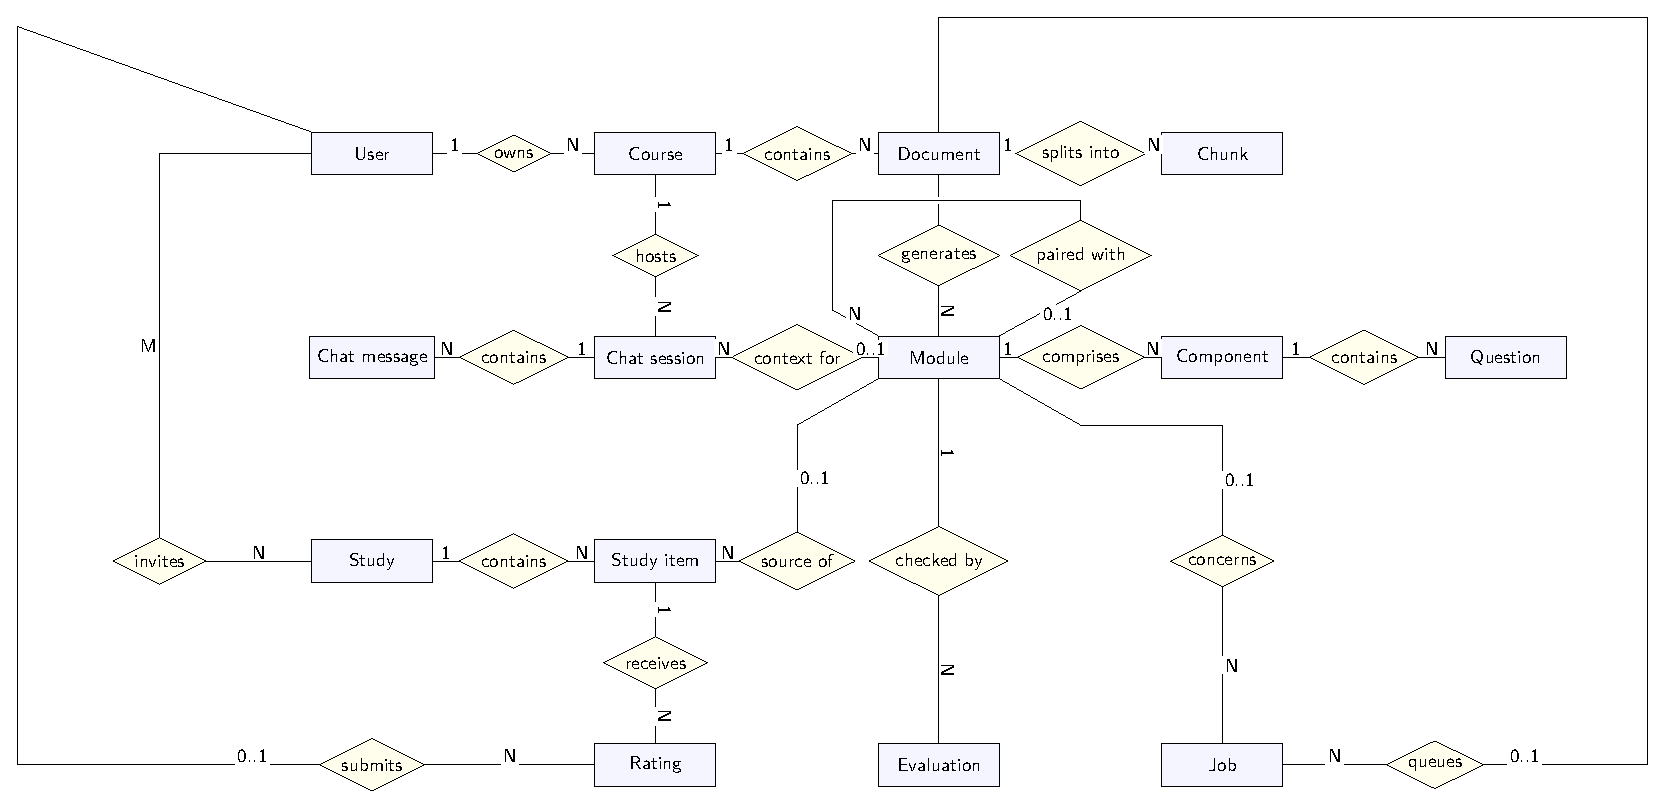
\includegraphics[width=\linewidth,height=.82\textheight,keepaspectratio]{diagrams/erd-overview.pdf}
\caption{Complete Chen overview: entities and relationships without attributes. M and N denote independently varying many sides (including zero); 1 denotes exactly one; 0..1 denotes an optional single entity.}
\label{fig:erd-overview}
\end{figure}
\end{landscape}
\needspace{10\baselineskip}
\subsection{Core relational mapping}
\begin{longtable}{|p{2.8cm}|p{7.0cm}|p{4.1cm}|}\caption{Core entity-to-table mapping.}\label{tab:schema}\\\hline
Table & Important columns and keys & Purpose / invariant\\\hline\endfirsthead
\hline Table & Important columns and keys & Purpose / invariant\\\hline\endhead
\code{users} & universally unique identifier (UUID) primary key (PK); unique email; password hash; active/admin/can-author flags; optional unique Moodle user ID; model preference; daily chat count & Local identity independent of Moodle confirmation\\\hline
\code{courses} & UUID PK; owner foreign key (FK) to users; name; nullable Moodle course ID & Owned authoring workspace; remote target may be shared by multiple app courses\\\hline
\code{course_members} & Composite PK (course, user); source & Read-only access for LTI learners (Section~\ref{sec:lti-learners})\\\hline
\code{documents} & UUID PK; course FK; filename; status; raw text; planner cache & Document processing and concept planning\\\hline
\code{chunks} & UUID PK; document/course FKs; ordered chunk index; content; source reference; vector(768) & Evidence unit and retrievable passage\\\hline
\code{modules} & UUID PK; document/course FKs; title; LO; Bloom level; sub-objectives; generation payload/models; optional paired-module FK & Saved module and experimental pairing\\\hline
\code{module_components} & UUID PK; module FK; type; JSONB content; unique (module, type) & One row per non-LO component type\\\hline
\code{questions} & UUID PK; component FK; stem; choices JSONB; answer key; explanation; position & Editable and exportable quiz/practice questions\\\hline\end{longtable}
The LO fields belong to \code{modules}, so the seven parts are six component types plus those fields. Component content is JSONB. The \code{course_id} copied onto chunks and modules makes course filters and row-level security cheap; a composite foreign key to \code{documents(id, course_id)} prevents such a row from naming a different course from its document. A unique (module, type) pair prevents two Content rows in one module, and explicit positions order chunks and questions.
\subsection{Operational and research mapping}
\begin{longtable}{|p{3.0cm}|p{6.6cm}|p{4.3cm}|}\caption{Operational and research entities.}\label{tab:05-data-2}\\\hline
Table & Key fields and links & Behavior\\\hline\endfirsthead
\hline Table & Key fields and links & Behavior\\\hline\endhead
\code{jobs} & Type, document/module references, step, status, payload, attempts, due time, lock metadata, last error and whether the system caused a failure & PostgreSQL-backed processing queue; nullable links depend on job type\\\hline
\code{evaluations} & Module FK, criterion, numeric score and notes & Pipeline checks; not formal blind ratings\\\hline
\code{chat_sessions} & Course FK, user FK and optional module FK & Course Q\&A or module-specific editing context; visible only to its user\\\hline
\code{chat_messages} & Session FK, role, text, citations and applied-edit flag & Persisted conversation and edit evidence\\\hline
\code{refresh_tokens} & User FK, unique token hash, expiry and revocation & Server-side session renewal control\\\hline
\code{studies} & Name, rubric version, status and JSONB invited email list & Draft/active/closed study organization\\\hline
\code{study_items} & Study FK, anonymous code, group, nullable source module FK and JSONB packet & Frozen blinded material; group hidden from raters\\\hline
\code{ratings} & Item FK, nullable user FK, rater kind, eight score/reason objects and notes & Human rating or LLM-judge slot, separate from pipeline checks\\\hline
\code{lti_platforms}, \code{lti_deployments} & Issuer, client id, key-set and token URLs; registered deployments & Platforms allowed to launch the tool\\\hline
\code{lti_identities}, \code{lti_contexts} & (platform, \code{sub}) to user; (platform, deployment, context) to course; roster address and last check & Who a launch is and which course it opens\\\hline
\code{lti_login_states}, \code{lti_launch_codes} & State and nonce with a 10-minute expiry; one-time launch code & Single use; kept in PostgreSQL so any task can finish a launch\\\hline\end{longtable}
A study item is a frozen packet; a RAG item also references its module, while the no-RAG item of a pair is self-contained. Ratings hold one row per human rater and item, and one per judge family and item. Foreign keys from studies use \code{RESTRICT}, so a module used in a study cannot be deleted silently; the API answers 409 instead.
\subsection{Citation and edit representation}
The server stores a \code{source_map} from codes such as S1 to a chunk id and its locator, and derives \code{inline_citations} from the saved Markdown with the character offsets of each claim and marker. Unknown codes are rejected. On the first edit, an \code{ai_original} object in the component keeps the version before editing, including the ordered questions and explanations; later edits do not change it.

\clearpage\section{Document, retrieval and generation pipelines}
\subsection{Ingestion: read, chunk and embed}
The API checks the format and the streamed size, stores the file in object storage and creates a document and a job. The worker then reads, chunks and embeds the document as separate steps, each retried on its own, and deletes the file after embedding (Figure~\ref{fig:ingestion}).
\diagram{ingestion}{Asynchronous ingestion with bounded retries.}{ingestion}
\subsubsection{Readers and source locators}
PDF is read with PyMuPDF and layout rules, with OCR for pages without text and the formula and figure repairs of Section~\ref{sec:results-extraction}. PPTX keeps slide text, tables, SmartArt and speaker notes. Recordings are transcribed by Whisper in 600-second windows. Every reader returns units of text with a page, slide or timestamp locator.
\subsubsection{Chunking and embedding}\label{sec:chunking}
Chunking follows the structure of the source before applying size limits. Short pages or slides can share a chunk, but no chunk spans more than two of them, so a citation still names a page. A long page is split at word boundaries and keeps its locator with a part index. Transcript segments are accumulated with their start and end times. DOCX and HTML use recursive splitting at paragraphs, lines and sentences\citep{recursivesplit}. The file name and the section or slide heading are prefixed to each chunk. Table~\ref{tab:chunk-parameters} gives the settings; lengths are estimated tokens, not the embedding model's tokenizer.
\begin{table}[H]\centering\small\caption{Structure-aware chunking and generation-context parameters.}\label{tab:chunk-parameters}
\begin{tabularx}{\linewidth}{|p{4.3cm}|p{2.1cm}|Y|}\hline
Parameter & Value & Meaning\\\hline
Content budget & 340 & Estimated tokens before title/heading prefix\\\hline
Narrative overlap & 50 & Estimated-token overlap in recursive splitting\\\hline
Page/slide grouping & Target 250; at most 2 & Flush at target; at most two distinct pages/slides; check 340 before merging\\\hline
Long-page overlap & 40 & Word-boundary split of oversized page/slide units\\\hline
Transcript target & 150 & Timestamp accumulation target; long captions split with zero overlap\\\hline
Context prefix & Title + heading & Omit redundant heading; recompute estimated length\\\hline
Generation neighbors & $\pm 2$ & Same-document physical neighbors retain individual source codes\\\hline
\end{tabularx}\end{table}
Semantic chunking was not adopted: Qu et al. found no consistent gain that justifies its cost\citep{semanticchunking}. Embeddings come from the local Qwen3 model through the gateway alias \code{embed-default}; queries carry the retrieval instruction and documents do not. Changing the model export requires re-embedding every chunk, which \code{scripts/reembed_chunks.py} does.
\subsection{Retrieval}
\subsubsection{Scope, candidates and ranking}\label{sec:retrieval-policy}
Module retrieval is limited to the selected document, chat to the course. Dense cosine search and BM25 each return ranked candidates, and RRF with constant 60 fuses them\citep{bm25,rrf}. The BM25 index is cached per scope and rebuilt when the chunk set changes.

A reranker reorders the candidates: Jina multilingual INT8 by default, or the hosted Jev model when configured (Section~\ref{sec:rerank-choice}). LO and Content rerank 30 candidates and use adaptive-$k$ with floor eight. Practice/Quiz retrieval for each sub-objective reranks 15 candidates and uses fixed $k=4$. Module-edit chat and course Q\&A use fixed $k=8$. Adaptive selection finds the largest adjacent gap within the leading 90\%, adds five and enforces floor eight\citep{adaptive}. A flat score distribution retains the search window. Each process sends at most two concurrent requests to a self-hosted reranker and retries a busy one (429, 502--504, connection errors) up to five times with backoff, so a busy reranker no longer restarts the job. A failed Jev call keeps the hybrid order and is logged for alerting; in chat, any rerank failure after two attempts keeps the hybrid order.
\subsubsection{Physical evidence and corrective retrieval}
Up to two neighbouring chunks on each side of a hit are added for Content; each keeps its own id and source code. Before Content is written, a relevance check judges whether the passages cover the LO and sub-objectives; if not, it rewrites the query once, merges the new passages and judges again\citep{correctiverag}. The confidence and retry count are stored with the module.
\subsection{Generation orchestration}\label{sec:generation}
Figure~\ref{fig:generation} shows retrieval and generation flow with physical inline citations.
\diagram{retrieval-generation}{Retrieval and generation flow with physical inline citations.}{generation}
\subsubsection{Planner and learning objectives}
The planner extracts up to eight ranked concepts from the first 8,000 characters of the document and is cached per document and output language. A generation takes the top concept, retrieves passages for it and writes the terminal LO, its Bloom level and the sub-objectives. Concepts that appear only after the first 8,000 characters are not considered, a known limit.
\subsubsection{Content and inline citations}
Content has one heading per sub-objective. The prompt gives each passage a code, and important statements carry a marker after them, for example \code{Heap insertion takes O(log n). [S2]}. The server rejects unknown codes, derives the character span of each claim and resolves each code to its chunk and locator, which the source panel shows beside the lesson.
\needspace{.55\textheight}
\subsubsection{Grounding and pedagogical freedom}\label{sec:grounding-policy}
Table~\ref{tab:grounding-policy} separates source-required knowledge from permitted instructional invention. This policy controls generation and defines the denominator of the source-support assessment.
\begin{table}[H]\centering\small\caption{Grounding policy for generated teaching material.}\label{tab:grounding-policy}
\begin{tabularx}{\linewidth}{|p{3.0cm}|Y|}\hline
Part & Grounding rule\\\hline
Lesson content & Facts, definitions and formulas come from supplied passages with \code{[S\#]} citations. The model may paraphrase and connect ideas, but adds no new knowledge.\\\hline
Illustrative examples & Worked examples and code may be created, labelled ``Illustrative example,'' and consistent with source concepts. Code is checked by execution in an isolated environment where possible.\\\hline
Practice and Quiz & New scenarios may elicit Apply/Analyze processes. Correct answers must be derivable from cited sources. Distractors may express model-generated common misconceptions and need no citation; each explanation cites the passage supporting the correct answer.\\\hline
Source gaps & Missing knowledge required by an objective is flagged to the lecturer instead of supplied from model knowledge.\\\hline
Support assessment & Assess source-required facts, correct answers and explanations. Exclude explicitly illustrative material and distractors from the support denominator.\\\hline
\end{tabularx}\end{table}
Source support and pedagogical quality are evaluated separately, so a configuration that asks only easy factual questions cannot win on support alone\citep{aqgreview}.
\subsubsection{Slides, example, questions and explanation}
Slides and Example are generated from the Content as structured objects. Each Practice and Quiz question retrieves its own passages for one sub-objective. A question writes its reasoning before its choices, then the explanation drawn from that reasoning; the Explanation component collects them, so it costs no extra call. Choices are checked for a single correct index and rebalanced when the correct answer is visibly the longest. Learner-facing text uses the chosen output language, English or Vietnamese.
\subsubsection{Self-check and comparison condition}
Content and each question have one self-check by the model, with one regeneration on failure; the results are stored with the module. Schema validation and citation checks always run. The no-RAG control of the evaluation runs the same steps with the source block removed (Section~\ref{sec:conditions}); control modules cannot be published.
\subsubsection{Concurrency within a module}
Question generation took about 75\% of a module's time on a real model (Section~\ref{sec:results-latency}). Questions are therefore generated five at a time (\code{QUESTION_CONCURRENCY}), and each worker process runs four jobs at once. Rate-limited model calls are retried individually by background jobs, as described in Section~\ref{sec:architecture}; every stage records its duration, model calls and tokens, which produced the timing tables of Section~\ref{sec:results}.
\subsection{Gateway routing and model control}
The gateway holds the provider keys and maps aliases to models (Table~\ref{tab:model-aliases}). In normal use an alias may fall back to another model after errors; experiment mode disables fallback, and every call records the alias requested and the model that served it.
\begin{table}[H]\centering\small\caption{Gateway aliases and their use in this project.}\label{tab:model-aliases}
\begin{tabularx}{\linewidth}{|p{2.6cm}|p{3.8cm}|Y|}\hline
Alias & Model & Used for\\\hline
\code{claude-fast} & Claude Haiku 5.5 & Generation latency and load tests\\\hline
\code{openai-fast} & GPT-6 Luna & Load tests\\\hline
\code{claude-pro}, \code{openai-pro} & Claude Sonnet 5.5, GPT-6.1 Sol & Planned rubric judges\\\hline
\code{gemini-fast} & Gemini 3.5 Flash-Lite & Chat evaluation, module pilot, formula re-reading\\\hline
\code{groq-pro} & GPT-OSS-120B on Groq & Load control, Ragas and claim judge\\\hline
\code{groq-qwen} & Qwen 3.8 27B on Groq & Preliminary rubric judge\\\hline
\code{transcribe} & Whisper large-v3 turbo on Groq & Transcription\\\hline
\code{embed-default} & Qwen3-Embedding-0.6B, local & Embedding\\\hline
\end{tabularx}\end{table}

\clearpage\section{Moodle integration and security}\label{sec:security}
\subsection{Identity linking and course authority}
The integration boundary consists of Moodle Web Services\citep{moodlews} and the \code{local_lms_bridge} plugin. The bridge provides identity, capability and publication contracts.

Local application identity and Moodle identity are independent. Registration does not prove control of a Moodle account. A link request produces an opaque request ID; a matching Moodle user must sign in and confirm on the Moodle side. The application then stores the confirmed Moodle user ID. A generic pending response prevents the link-request response from revealing whether the entered email matches an active account. Missing and ambiguous emails receive pending requests with the same externally visible shape; only legitimate confirmation may reveal identity.

A confirmed identity does not automatically grant access to every Moodle course. The bridge queries course authoring capabilities and verifies the requested actor in the course context. The author ID is propagated on creation calls. The bridge also checks relevant activity/question capabilities in its external handlers. The application administrator is not treated as a Moodle administrator solely because the local admin flag is true. Rights can be revoked externally, so publication verifies them immediately before activity writes.
\subsection{Publication mapping and sequence}
The Book receives navigable lesson material, including the LO and usable generated content. Practice is published as a quiz with immediate feedback; the assessment Quiz uses deferred feedback. Question stems, choices and explanations are exported from the live saved question data. The target section is chosen by the author. Moodle's Book and Quiz remain the actual learner-facing activities\citep{moodlebook,moodlequiz}.
Figure~\ref{fig:moodle} shows publication sequence and permission checks. Book and subsequent quiz writes are separate remote operations.
\diagram{moodle-sequence}{Publication sequence and permission checks. Book and subsequent quiz writes are separate remote operations.}{moodle}
The application sanitizes HTML through an allowlist before transmission and returns created activity IDs. Book, Practice and Quiz are separate remote operations. If a later operation fails, earlier activities can remain. The publication design records external IDs and per-step state, expose partial success and support safe resumption during recovery.
\subsection{LTI 1.3 launch}\label{sec:lti}
The advisor asked for the Moodle-to-LTI-tool model. GENAILMS now acts as an LTI 1.3 tool: an instructor opens an External tool activity in a Moodle course and arrives signed in, in the matching course, without a password. The bridge plugin is kept for publishing Book and Quiz activities, because a standard LTI tool cannot create them.
\begin{enumerate}[nosep]
\item Moodle calls \code{/api/lti/login}. The tool stores a \code{state} and \code{nonce} in PostgreSQL with a 10-minute expiry and redirects to Moodle's authorization endpoint.
\item Moodle posts a signed \code{id_token} to \code{/api/lti/launch}. The tool consumes the state, so it is usable once even when the launch is rejected, and verifies the RS256 signature with Moodle's key set, which is cached and fetched again when an unknown key id appears.
\item It checks issuer, audience (and \code{azp} when there are several audiences), expiry and issue time with 60 s of clock skew, nonce, a registered deployment, version \code{1.3.0}, message type \code{LtiResourceLinkRequest} and the presence of a course context.
\item It finds or creates the user by the pair of platform and \code{sub}, and the course by platform, deployment and context id, then redirects to the frontend with a one-time code in the URL fragment, which the frontend exchanges for the same tokens a password login gives.
\end{enumerate}
Email does not identify an LTI user, because a launch does not prove control of an address here. For the project's own Moodle, the LTI \code{sub} and context id are Moodle's user and course ids, guaranteed by Moodle's signature, so a launch reuses the account and course already linked through the plugin instead of creating second ones. The launch was run end to end against Moodle 5.2.3 in an isolated stack: the instructor entered and saw the course, a second launch reused the same account and course, a student was refused, and the stored Moodle ids matched. Rejection cases (wrong signature, audience, expiry, nonce or deployment, replayed state, reused code) are tested with a fake platform signing with a real RSA key.

Current limits: each course belongs to one instructor; Deep Linking and grade return are not implemented, because the tool publishes modules through the plugin and does not grade students; and the login state is not bound to the browser, so an attacker could make a victim sign in to the attacker's own tool account (login cross-site request forgery). Binding the state to a \code{SameSite=None} cookie when the tool opens in a new window would prevent it. The tool should be opened in a new window: inside an iframe, browsers partition storage, so the session would not be shared with a directly opened tab.
\subsection{Student access through LTI}\label{sec:lti-learners}
A student who opens the same External tool activity may chat with the course's material and do nothing else. Three decisions were made before the change: the lecturer does not read students' chats, a student may send 30 chat messages per day, and a student's launch is refused until the instructor has opened the tool once, because the course does not exist in the tool before that.

Until this change, ``a course I can see'' and ``a course I own'' were the same condition in every row-level security policy. Course membership separates them (Table~\ref{tab:member-access}):
\begin{itemize}[nosep]
\item A \code{course_members} table holds (course, user) pairs. A row can be inserted only by the member themself and only for a course that an LTI context opens, so membership comes only from a signed launch. The \code{courses} policy reads membership through a \code{SECURITY DEFINER} function, because PostgreSQL refuses a policy on \code{courses} that reads \code{course_members} while the policy on \code{course_members} reads \code{courses}.
\item Members get policies for \code{SELECT} only, on \code{courses}, \code{documents} and \code{chunks}. Every write still requires the owner; modules, jobs and their children stay owner-only.
\item \code{chat_sessions} gained a user column. A session is visible only to the person who had it, in a course that person can see; existing sessions were assigned to the course owner, who had them.
\item \code{users.can_author} is false for an account created by a Learner launch and set true by an Instructor launch. Creating a course requires it, and the daily chat counter applies only to accounts that cannot author.
\end{itemize}
\begin{table}[H]\centering\small\caption{What a course member can reach.}\label{tab:member-access}
\begin{tabularx}{\linewidth}{|p{4.2cm}|Y|Y|}\hline
Resource & Owner & Member through LTI\\\hline
Course, documents, chunks & Read and write & Read, in the database; the API exposes them only through chat\\\hline
Modules, jobs, publication & Read and write & None\\\hline
Course chat & Own sessions & Own sessions, 30 messages per day\\\hline
Other people's chats & None & None\\\hline
\end{tabularx}\end{table}
The API keeps the owner check on every route except chat, which accepts an owner or a member. \code{/lti/session} returns the course role, and the frontend opens a member's launch on a chat-only page; an author page reached by a student account redirects there. A student who requests a route the lecturer can reach receives 404, as for any missing resource.

The policies are tested as SQL under the runtime role: what a member reads, that it cannot change or add, and who sees which chat. Loosening the \code{documents} policy back to its previous condition makes three of these tests fail. Launch tests cover a student before the instructor (refused), a student who joins and can only chat, one membership after repeated launches, the daily limit, an author who launches as a learner and a student who later becomes an instructor. Against Moodle 5.2.3, a student before the teacher received 400; the teacher became the owner; the student then became a member, chat returned 200, the document list 404, and one membership row was stored.

A launch adds a member but never says that one has left. The worker therefore reads the course roster through the LTI Names and Role Provisioning Services 2.0. The roster address comes from the \code{namesroleservice} claim of the latest launch and must have the issuer's origin, because the access token is sent to it. The tool obtains that token with an OAuth~2 client-credentials grant, signing its assertion with its own RSA key; the public key is served at \code{/api/lti/jwks} with an RFC~7638 thumbprint as its key id. Every five minutes the worker reads, page by page, the roster of each course not checked for an hour, and removes the members who are no longer listed as active learners or instructors; a suspended enrolment counts as gone. The next request of a removed student finds no course, because membership is enforced by row-level security. Nobody is removed when the result is uncertain: a failed or refused request, a next page outside the platform, an empty roster or a course whose context has no roster address leaves membership unchanged until the next check.

Tests use a fake platform that verifies the assertion with the key set the tool publishes, and cover departure, suspension, roles the tool does not serve, several pages, one read per cycle and each case that must remove nobody. Against Moodle 5.2.3, with a key generated for the run, the worker read the roster and removed nobody while the student was enrolled, then removed exactly that student after they were unenrolled; the teacher remained the owner. A student therefore loses access within about one hour and five minutes of leaving the course. Where the platform does not offer the service or the tool has no key, the earlier limit applies: the account keeps chatting until the session of its last launch expires, at most 14 days later.
\subsection{Authentication and session security}
Passwords are stored as bcrypt hashes\citep{bcrypt}. Access tokens are JSON Web Tokens\citep{jwt} valid for 15 minutes and kept in memory by the browser; the active and admin flags are read from the database on every request, so disabling an account takes effect at once. Refresh tokens are random values stored as SHA-256 hashes, rotated on each use and sent in a Secure, HttpOnly, SameSite cookie limited to the refresh endpoint; renewal also checks the origin and a CSRF token. Logout revokes the refresh token. Rendered Markdown is sanitised and a restrictive content security policy limits cross-site scripting. Production settings refuse default secrets.
\subsection{Row-level security and ownership}
Authorisation is checked on the server and denies by default\citep{owaspaccess}, in the API and again by PostgreSQL row-level security (RLS). Table owners bypass row policies\citep{postgresrls}, so requests use a separate runtime role, and the user id is set as a transaction-local setting at the start of every transaction. Course-owned content is filtered by policies; course members have separate read-only policies (Section~\ref{sec:lti-learners}). The worker has a separate role with restricted table grants; it is a trusted service boundary, not a user session. It is exempted from row-level security by an explicit policy on each table rather than by the \code{BYPASSRLS} attribute, which the non-superuser master role of RDS cannot set (Section~\ref{sec:architecture}). No application role has \code{BYPASSRLS}, and a test fails when a new table with row-level security lacks the worker policy.

RLS filters rows but cannot hide columns, so raters read studies through views that omit the group and the source module. A rater can read and write only their own ratings. Administrative job retry goes through a narrow database function, which gives the administrator no access to course content.
\subsection{Indirect prompt injection}\label{sec:prompt-injection}
Uploaded material is untrusted input to the model: a document can contain text written as an instruction, such as ``ignore the rules above''\citep{owaspprompt}. Three controls are implemented. Every prompt that receives source passages wraps each passage in a block marked as data, not instructions, and contains a rule that instructions found inside the sources must be treated as course content and not followed. Lecturer guidance is wrapped the same way and may change emphasis and wording but not the grounding rules. The model's output is never trusted: it is validated against a schema, its citation codes must exist in the prompt, HTML sent to Moodle passes an allowlist, and the model decides no authorisation and starts no publication. Two further controls are designed but not implemented: flagging instruction-like passages at ingestion for the lecturer, and datamarking the source text\citep{spotlighting}. Delimiters and rules reduce the risk; they are not a security boundary, which is why authorisation never depends on model output.
\subsection{Threats, controls and verification targets}
Table~\ref{tab:07-moodle-security-1} maps each threat to its control and its test.
\begin{longtable}{|p{3.0cm}|p{5.8cm}|p{5.1cm}|}\caption{Security controls and their limits.}\label{tab:07-moodle-security-1}\\\hline
Threat & Control & Verification\\\hline\endfirsthead
\hline Threat & Control & Verification\\\hline\endhead
Cross-owner object access & Ownership checks, course/document filters, composite FKs and RLS; uniform missing-resource response & Direct API and runtime-role DB probes across owners and after transaction restart\\\hline
Account enumeration & Generic Moodle pending link response & Equivalent status and expiry for matching, missing and ambiguous emails; transport errors remain distinct\\\hline
Unsafe rendered content & Moodle HTML allowlist; structured model output & Markdown preview and exported activity XSS cases, including source text\\\hline
Resource exhaustion & Streamed upload limits, JSON body limit, route limits and daily generation cap for untrusted accounts & Concurrent uploads/jobs, provider quota exhaustion, CPU/RAM and fair scheduling\\\hline
Indirect prompt injection & Sources and guidance delimited as data, a rule against embedded instructions, output validation (Section~\ref{sec:prompt-injection}) & Adversarial documents\\\hline
Credential exposure & Provider keys stay at gateway; separate DB roles; secret-aware configuration fields & Production configuration, logs, rotation and backup access\\\hline
Publication misuse & Confirmed actor plus fresh Moodle capability checks & Unlinked, revoked, suspended and wrong-course scenarios\\\hline
Student overreach & Membership only from a signed launch; member policies for \code{SELECT} only; chats per person; 30 messages per day (Section~\ref{sec:lti-learners}) & Runtime-role SQL tests and Moodle 5.2.3 run done; roster checks remove a departed student within about an hour\\\hline
Blinding failure & Restricted views, own-rating policies and snapshots & Response field audit and packet-text leakage review\\\hline
\end{longtable}
JSON bodies are limited to 1 MB and uploads have their own streamed limits (NFR07). Production hides the API documentation and sets security headers. Selected source text is sent to the model provider; embedding stays on the project's own server. The optional Jev reranker would send the query and candidate chunks to TypeSafe in the United States, so it stays disabled until the university agrees.

\clearpage\section{API design summary}\label{sec:api}
\subsection{Resource and asynchronous contracts}
The application programming interface (API) uses FastAPI and JavaScript Object Notation (JSON) resources with local UUIDs; uploads use multipart data and PPTX export returns binary content. Moodle IDs remain remote identifiers. OpenAPI is exposed in development and disabled publicly in production. Upload and generation responses identify durable jobs for polling. Identity-link requests return an opaque pending request, with confirmation checked through a separate state resource.
\par
Table~\ref{tab:08-api-1} presents representative endpoint groups; resource contracts and authorization.
\begin{longtable}{|p{6.6cm}|p{7.3cm}|}\caption{Representative endpoint groups; resource contracts and authorization.}\label{tab:08-api-1}\\\hline
Method / resource & Contract and authorization\\\hline\endfirsthead
\hline Method / resource & Contract and authorization\\\hline\endhead
\code{POST /auth/register}, \code{/auth/login}, \code{/auth/refresh}, \code{/auth/logout} & Validate credentials; issue, renew or revoke the session\\\hline
\code{GET, POST /courses}; \code{DELETE /courses/{id}} & Owned workspaces; deletion conflicts with protected study sources\\\hline
\code{GET /courses/moodle/courses}; \code{POST /courses/{id}/link-moodle} & Confirmed identity and remote course-author rights\\\hline
\code{POST /documents}; \code{GET /documents?course_id=...}; \code{GET /documents/jobs/{job_id}} & Upload/list owned source and poll processing\\\hline
\code{POST /modules/generate}; \code{GET /modules/jobs/{job_id}} & Freeze source/model/language/guidance settings; poll to a saved module ID\\\hline
\code{GET, PATCH /modules/{id}}; \code{PATCH /modules/{id}/components/{cid}}; \code{PATCH /modules/{id}/questions/{qid}} & Owner reads/edits; original retention, citation validation and synchronized explanations\\\hline
\code{POST /modules/{id}/chat-edit}; \code{GET /modules/{id}/slides.pptx} & Authorized structured AI edit or current Slides download\\\hline
\code{POST /modules/{id}/publish-to-moodle} & Owned RAG module, confirmed actor and authorized target\\\hline
\code{POST /moodle/account/link-requests}; \code{GET, DELETE /moodle/account} & Generic pending identity request, poll confirmed state or unlink\\\hline
\code{POST /courses/{id}/chat}; \code{GET /courses/{id}/chat/{session}/history} & Owner-only course Q\&A, source citations and conversation history\\\hline
\code{POST /courses/{id}/chat/stream}; \code{GET /courses/{id}/chat/latest} & Owner-only streamed answer as SSE events \code{session}, \code{delta}, \code{done} or \code{error}; the last used course chat, so a reload continues it\\\hline
\code{GET, POST /lti/login}, \code{POST /lti/launch}, \code{POST /lti/session}, \code{GET /lti/jwks} & LTI 1.3 login initiation, signed launch, one-time code exchange and the tool's key set (Section~\ref{sec:lti})\\\hline
\code{GET /health}; \code{GET /ready} & Process liveness for the container; database readiness with a 2 s deadline for the load balancer\\\hline
\code{GET /models}; \code{PUT /models/default} & Available aliases and user preference\\\hline
\code{POST /jobs/{id}/retry}; \code{GET /admin/jobs/failed}; \code{POST /admin/jobs/retry} & Own-job recovery or narrow admin recovery scope\\\hline
\code{GET /admin/users} and account actions & Administrator-only account management\\\hline
\code{POST, GET /studies}; \code{POST /studies/{id}/items}; \code{PUT /studies/{id}/raters} & Admin prepares paired snapshots and invitations\\\hline
\code{GET /studies/mine}; \code{GET /studies/mine/{id}/items}; \code{PUT /studies/mine/{id}/items/{item}/rating} & Invited rater reads blinded packets and writes own rating only\\\hline\end{longtable}
\subsection{Validation and client state}
Authentication failures normally return 401; missing/non-owned resources use 404. Validation uses 422, oversized uploads 413, protected/concurrent-state conflicts 409 and rate limits 429. Catalog unavailability maps to 503 without revealing its internal URL. A task at its concurrent chat-stream limit also answers 503. A stream that fails after its response has started reports an \code{error} event, because the status code has already been sent. Moodle helpers distinguish remote identity, capability and service failures.

Clients poll job outcomes after submission and open a module only after completion. They distinguish a pending link, confirmed identity and course-specific permission. Source review and saved edits precede export/publication. Generation settings and served-model history belong in researcher manifests; ordinary screens need clear state and actions rather than raw internal fields.

\clearpage\section{UI/UX design}\label{sec:ui}
\subsection{Navigation and interaction principles}
The GENAILMS interface uses Vietnamese microcopy and role-specific views. The authoring flow is dashboard $\rightarrow$ documents $\rightarrow$ generation $\rightarrow$ review/edit $\rightarrow$ publication. Each screen emphasizes one primary action; menus, tooltips and expandable rows hold secondary detail. Citation inspection and AI chat sit beside the lesson, preserving reading context during review. Status combines words, icons and colour.

\par
Table~\ref{tab:09-ui-1} presents interface typography, spacing and accessibility rules.
\begin{table}[H]\centering\small\caption{Interface typography, spacing and accessibility rules.}\label{tab:09-ui-1}
\begin{tabularx}{\linewidth}{|p{3.0cm}|Y|Y|}\hline
Concern & Design rule & Design rationale\\\hline
Readability & IBM Plex Sans body 16/24 px; small 14/20; reading 16/27 & Readable text and Vietnamese diacritics at desktop and mobile sizes\\\hline
Hierarchy & Newsreader page titles 28/36; sans section/dialog headings 20/28 & Distinct page hierarchy with consistent functional headings\\\hline
Control visibility & Input borders \code{\#8F8778}; navy focus ring & Measured contrast 3.56:1 on white, 3.35:1 on cream, 3.12:1 on subtle: above the 3:1 control-border target\citep{wcag}\\\hline
Rhythm & 4/8 spacing scale; 1120 px content cap; text at most 72ch & Consistent alignment and manageable reading length\\\hline
Feedback & Text errors, labelled status, empty/loading/error states and mobile actions & Avoid colour-only meaning and show the next useful action\\\hline
\end{tabularx}\end{table}

Keyboard order, dialog focus, live announcements and task completion are acceptance criteria. Table~\ref{tab:screen-design} relates the interaction surfaces to the use cases and design decisions. Vietnamese microcopy is retained in the figures; the surrounding English gloss identifies the primary action. Focused crops enlarge the controls and evidence needed for each discussion.
\begingroup\small
\begin{longtable}{|p{2.8cm}|p{2.1cm}|p{3.7cm}|p{5.1cm}|}\caption{Screen interactions and design rationale.}\label{tab:screen-design}\\\hline
Screen & UC / FR & Primary action & Key design decision\\\hline\endfirsthead
\hline Screen & UC / FR & Primary action & Key design decision\\\hline\endhead
Access & UC01 / FR01 & Sign in or register & Labelled fields, recoverable validation\\\hline
Courses & UC02--03 / FR02--03 & Open course; upload source & Ownership context and visible processing state\\\hline
Generation & UC04,15 / FR04,15 & Confirm model, language and guidance & Saved preference preselects a per-request choice\\\hline
Source review & UC05 / FR05 & Inspect citation & Claim and original evidence stay adjacent\\\hline
Editing & UC06--07 / FR06--07 & Apply edit; download slides & Review context and saved-state feedback\\\hline
Publication & UC08--09 / FR08--09 & Link account; publish & Destination, capability and partial-result visibility\\\hline
Administration & UC10--12 / FR10--11,13 & Manage accounts, jobs, studies & Narrow role-specific actions\\\hline
Rating & UC13 / FR12 & Score anonymous packet & Stable order, criterion reasons and source access\\\hline
Course Q\&A & UC14 / FR14 & Enter course conversation & Course-scoped history and source citations; workspace entry\\\hline
Mobile / states & UC01--15 & Complete or recover a task & One-column actions; text and icons reinforce colour\\\hline
\end{longtable}\endgroup

\needspace{.42\textheight}
The login form in Figure~\ref{fig:ui-screen-01} makes the credential fields and the primary sign-in action explicit. ``Đăng nhập'' means ``Sign in''; ``Mật khẩu'' means ``Password''.
\begin{figure}[H]\centering
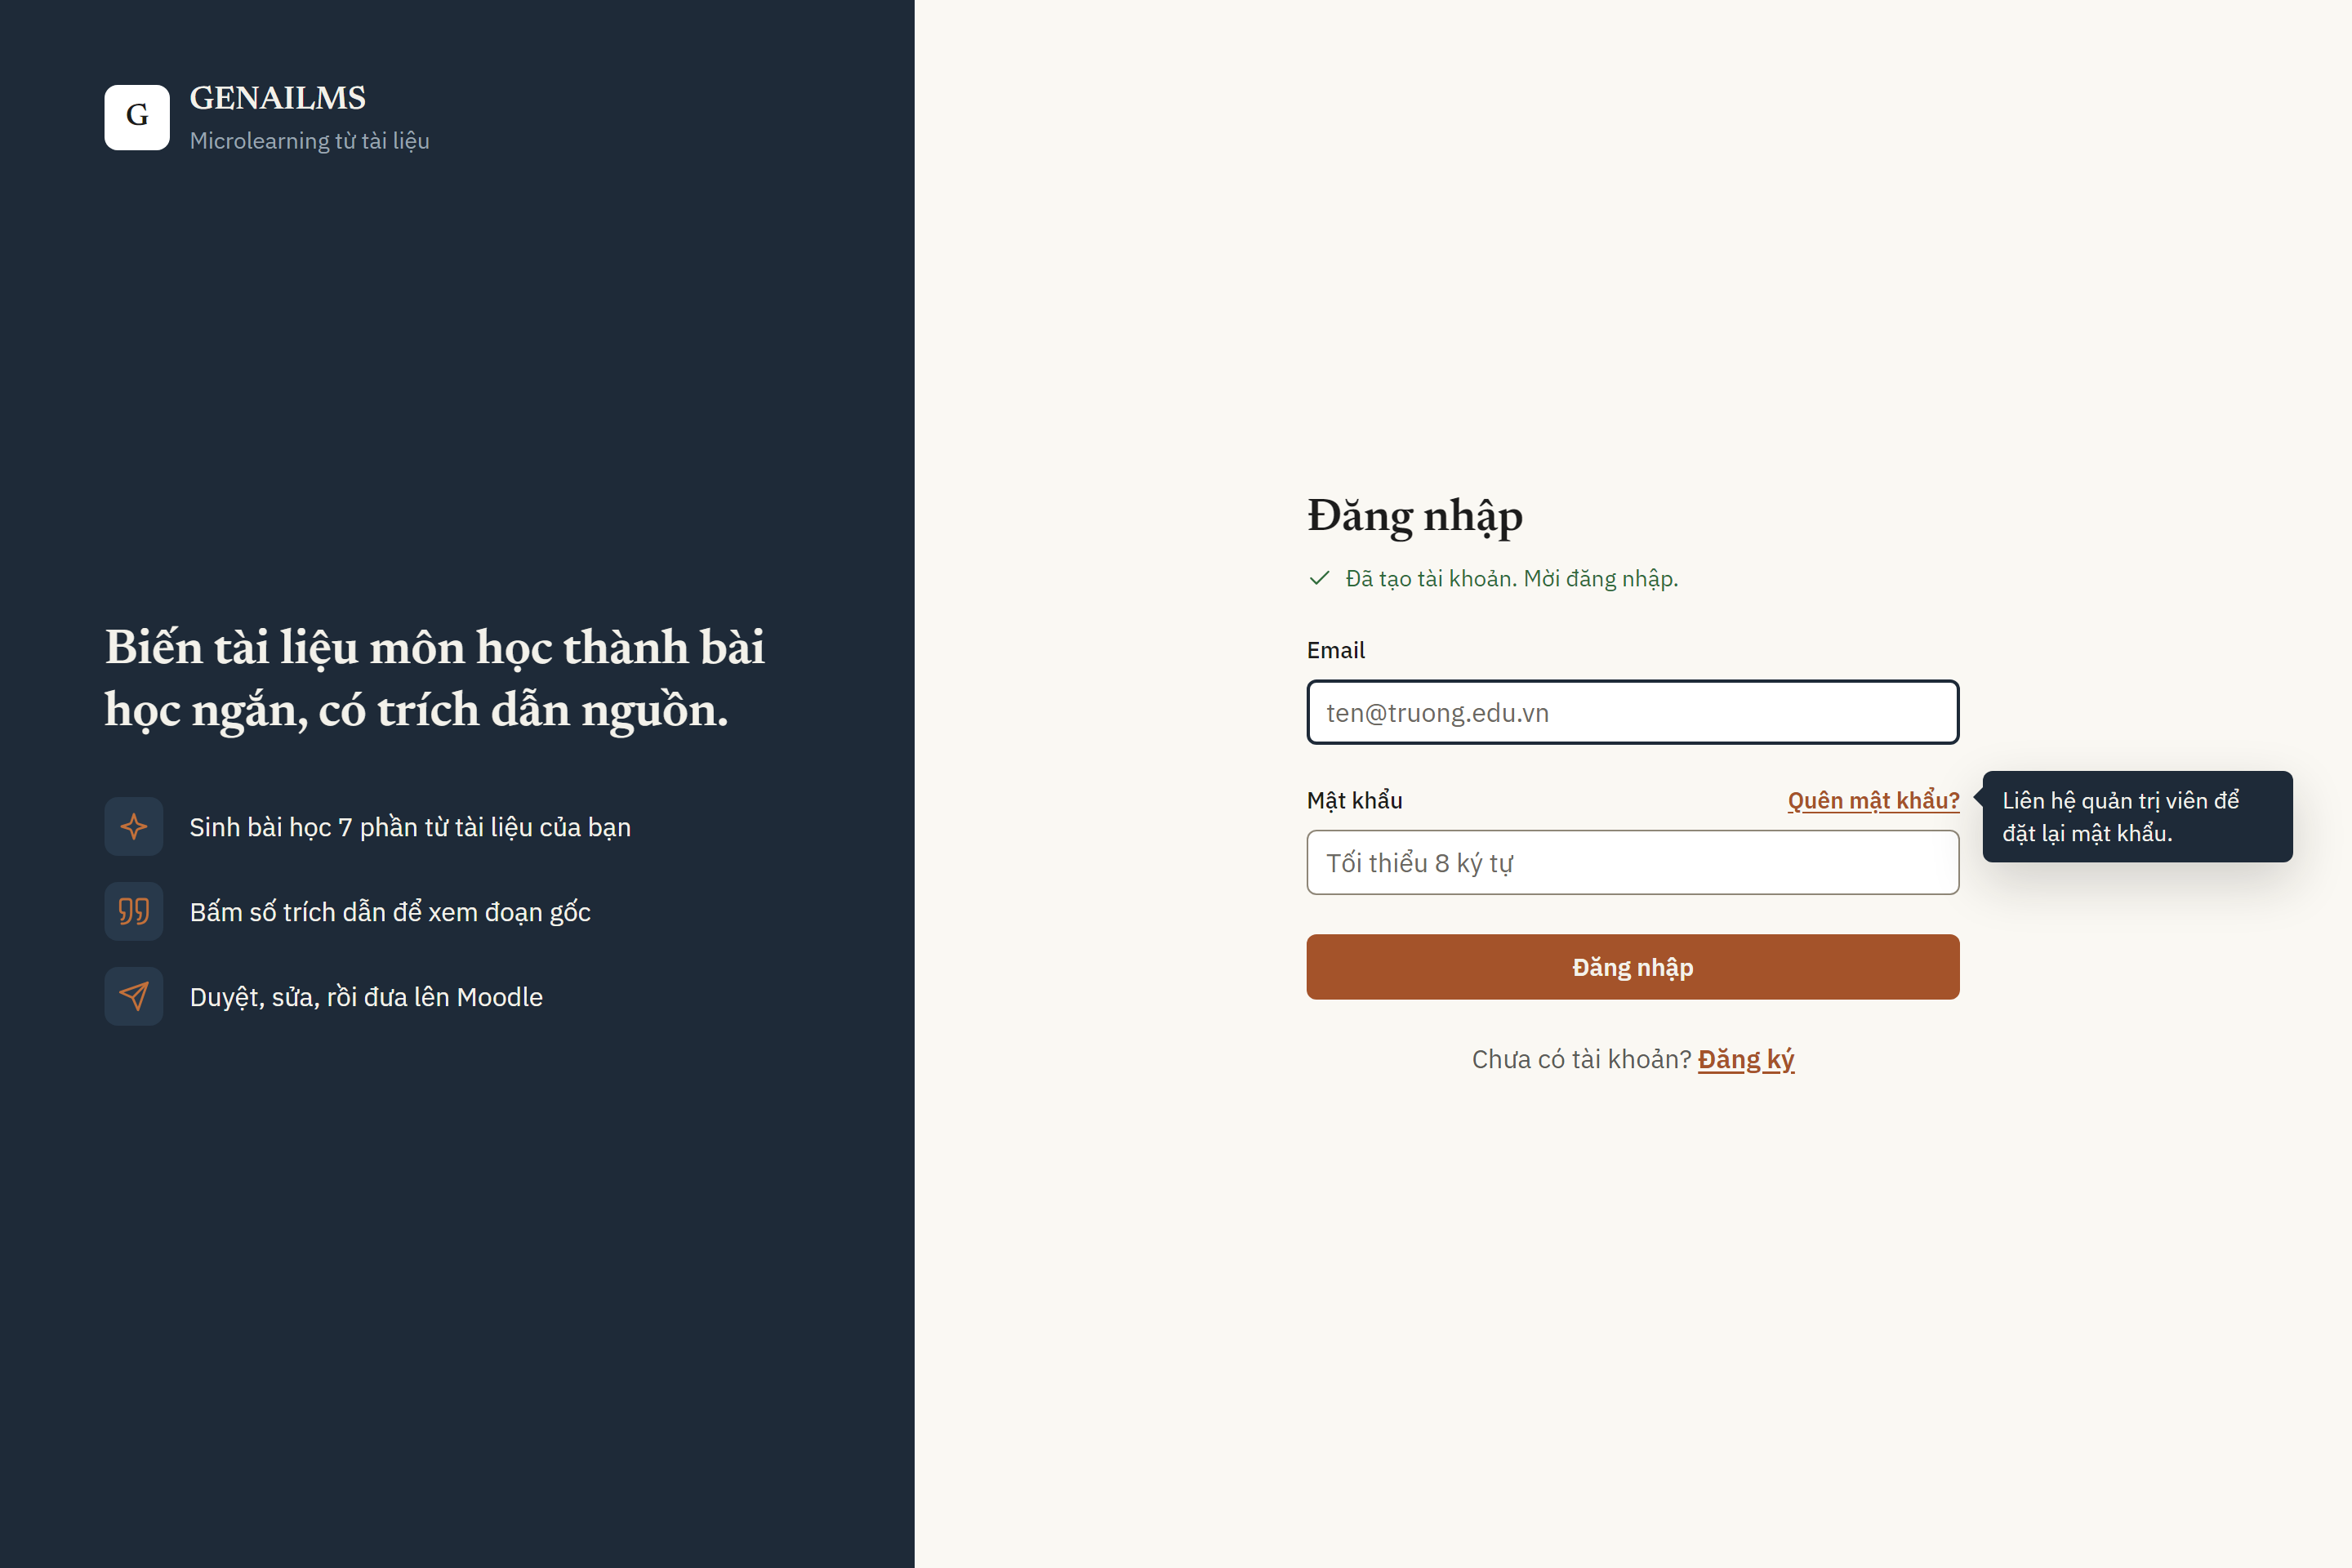
\includegraphics[width=\linewidth,height=.34\textheight,keepaspectratio,viewport={1550 500 2830 1450},clip]{graphics/ui/01-login.png}
\caption{Credential entry and sign-in feedback.}\label{fig:ui-screen-01}
\end{figure}

\needspace{.42\textheight}
Figure~\ref{fig:ui-screen-02} presents registration with persistent labels and repeated-password validation. ``Đăng ký'' means ``Register''; validation remains next to the field that needs correction.
\begin{figure}[H]\centering
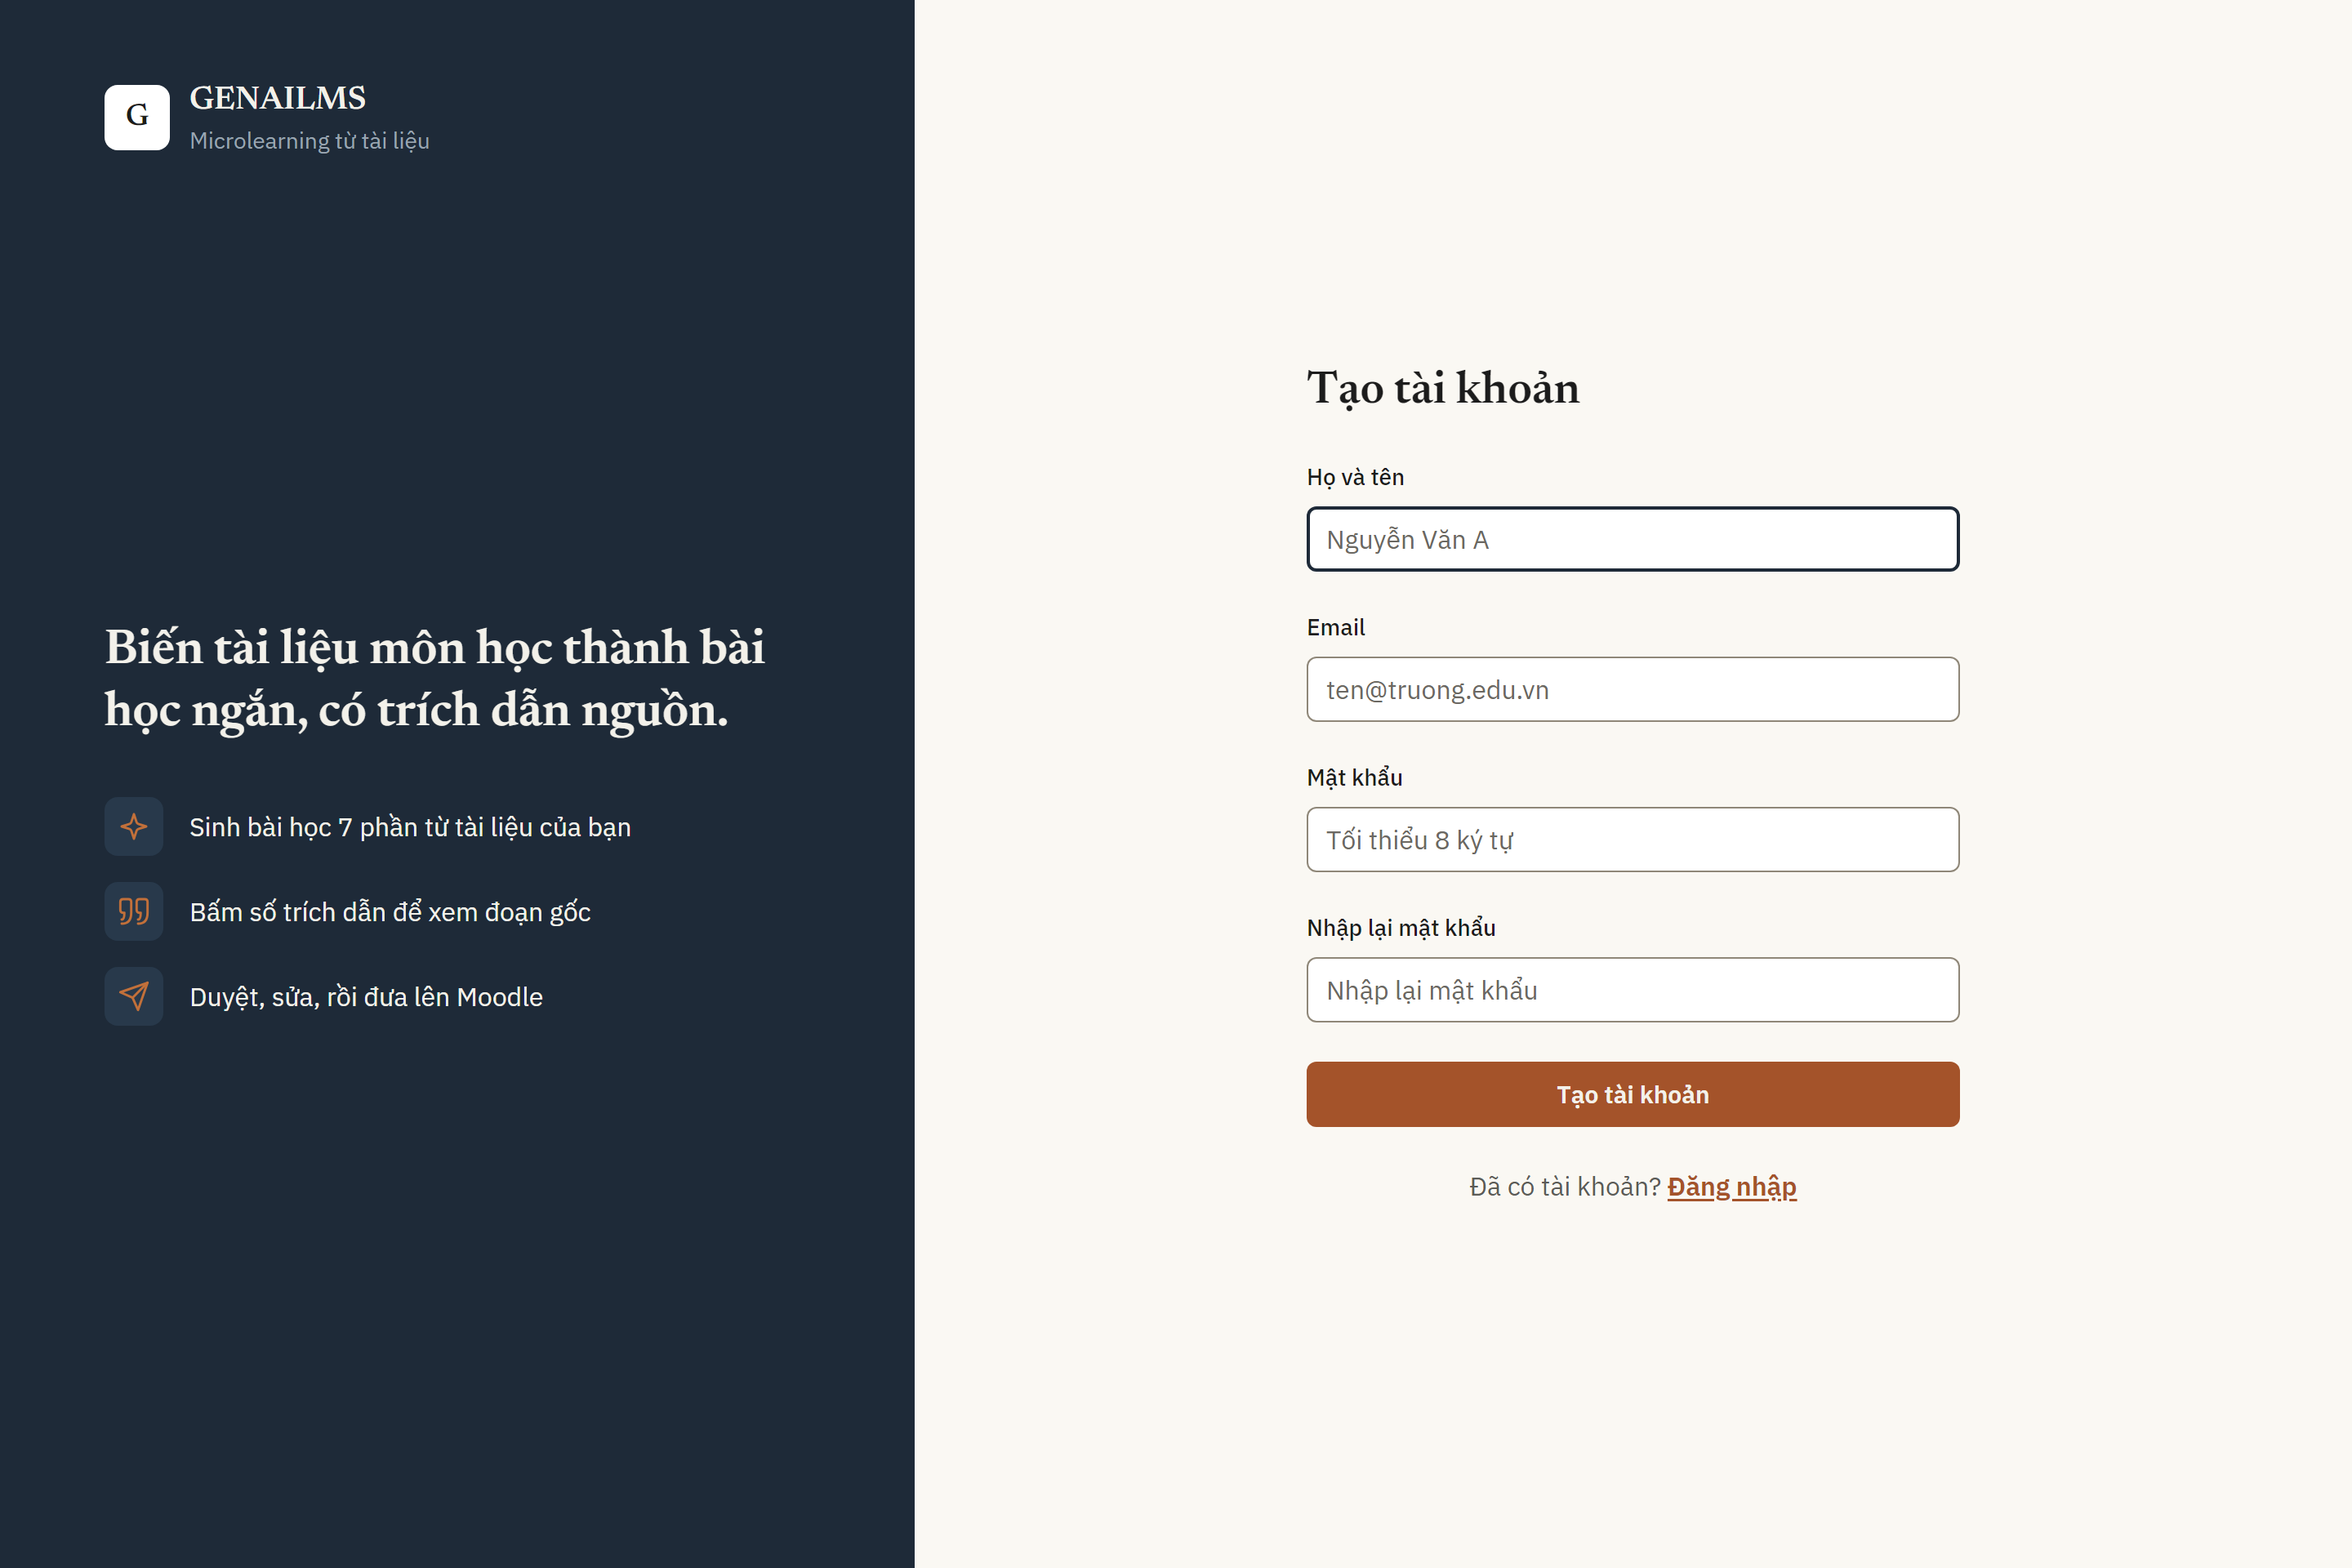
\includegraphics[width=\linewidth,height=.34\textheight,keepaspectratio,viewport={1560 420 2440 1010},clip]{graphics/ui/02-register.png}
\caption{Registration and labelled validation.}\label{fig:ui-screen-02}
\end{figure}

\needspace{.42\textheight}
Figure~\ref{fig:ui-screen-03} organizes the author's owned courses as selectable workspaces. ``Tạo môn học'' means ``Create course''; each card combines the course identity and a compact activity summary.
\begin{figure}[H]\centering
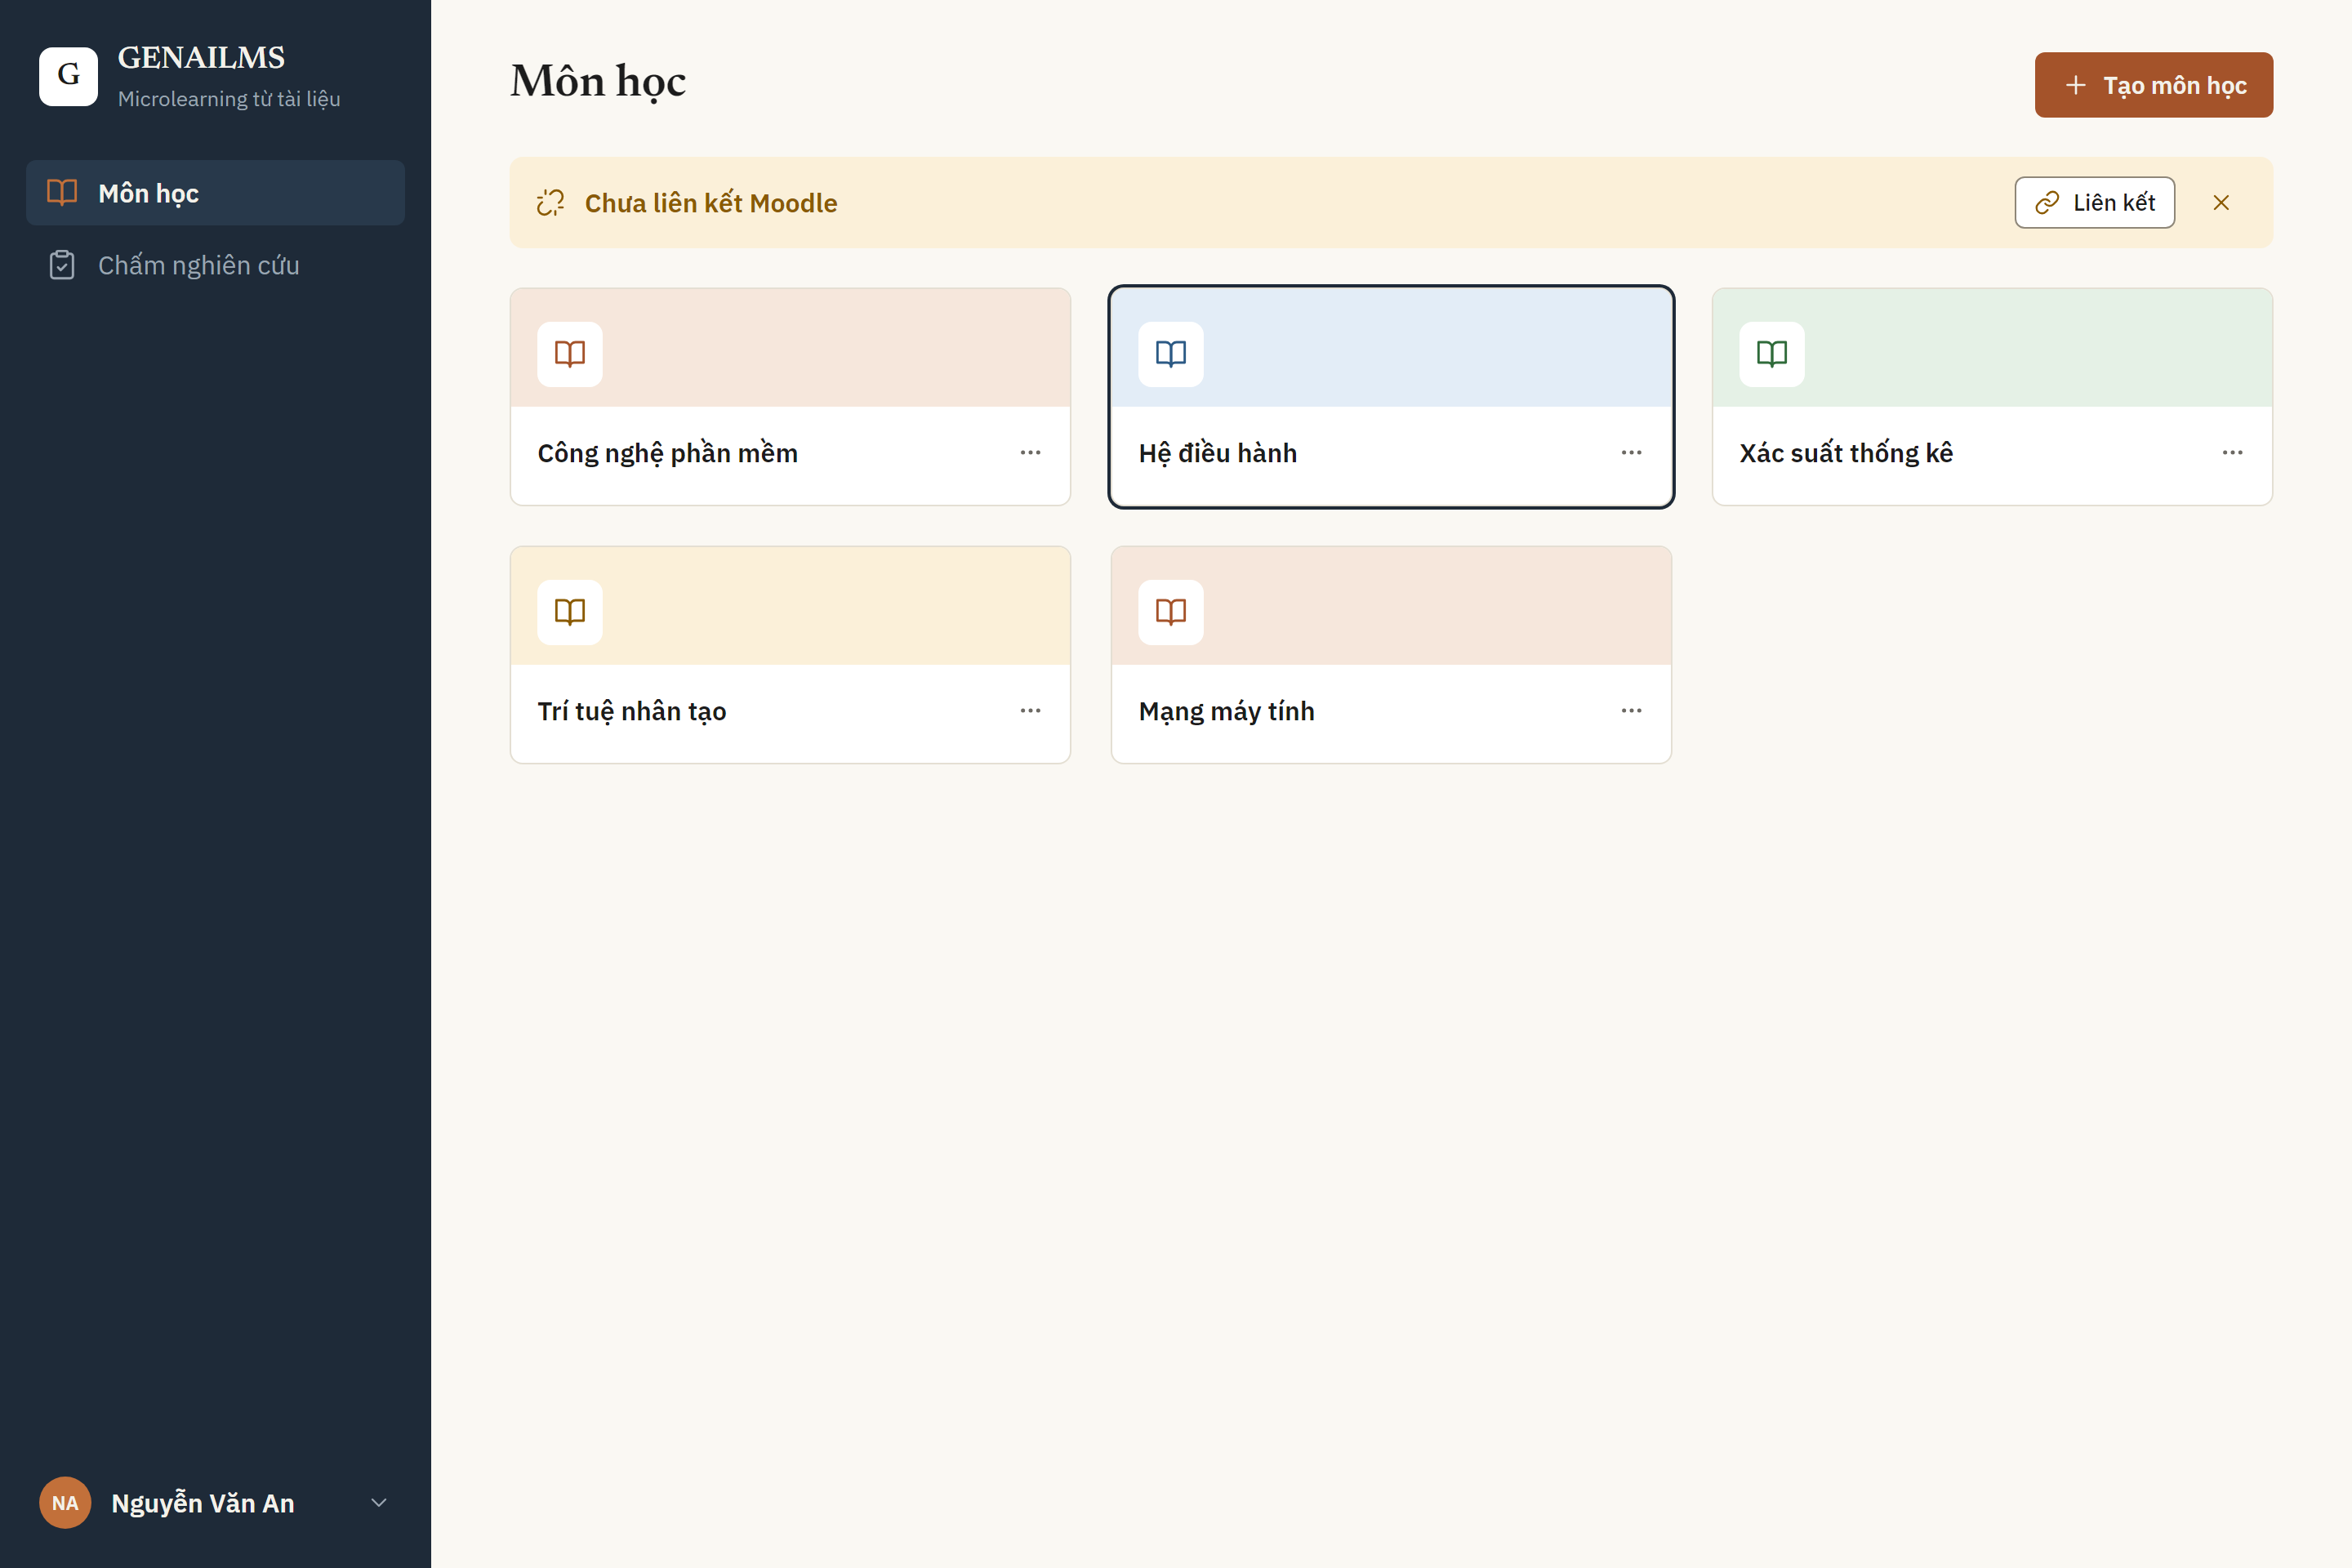
\includegraphics[width=\linewidth,height=.34\textheight,keepaspectratio,viewport={600 960 2070 1600},clip]{graphics/ui/03-course-list-dashboard.png}
\caption{Owned-course workspace selection.}\label{fig:ui-screen-03}
\end{figure}

\needspace{.42\textheight}
The workspace in Figure~\ref{fig:ui-screen-04} combines document status, generation actions and course context. ``Sẵn sàng'' means ``Ready'', while ``Đang xử lý'' means ``Processing''; course Q\&A is entered from this owned-workspace context.
\begin{figure}[H]\centering
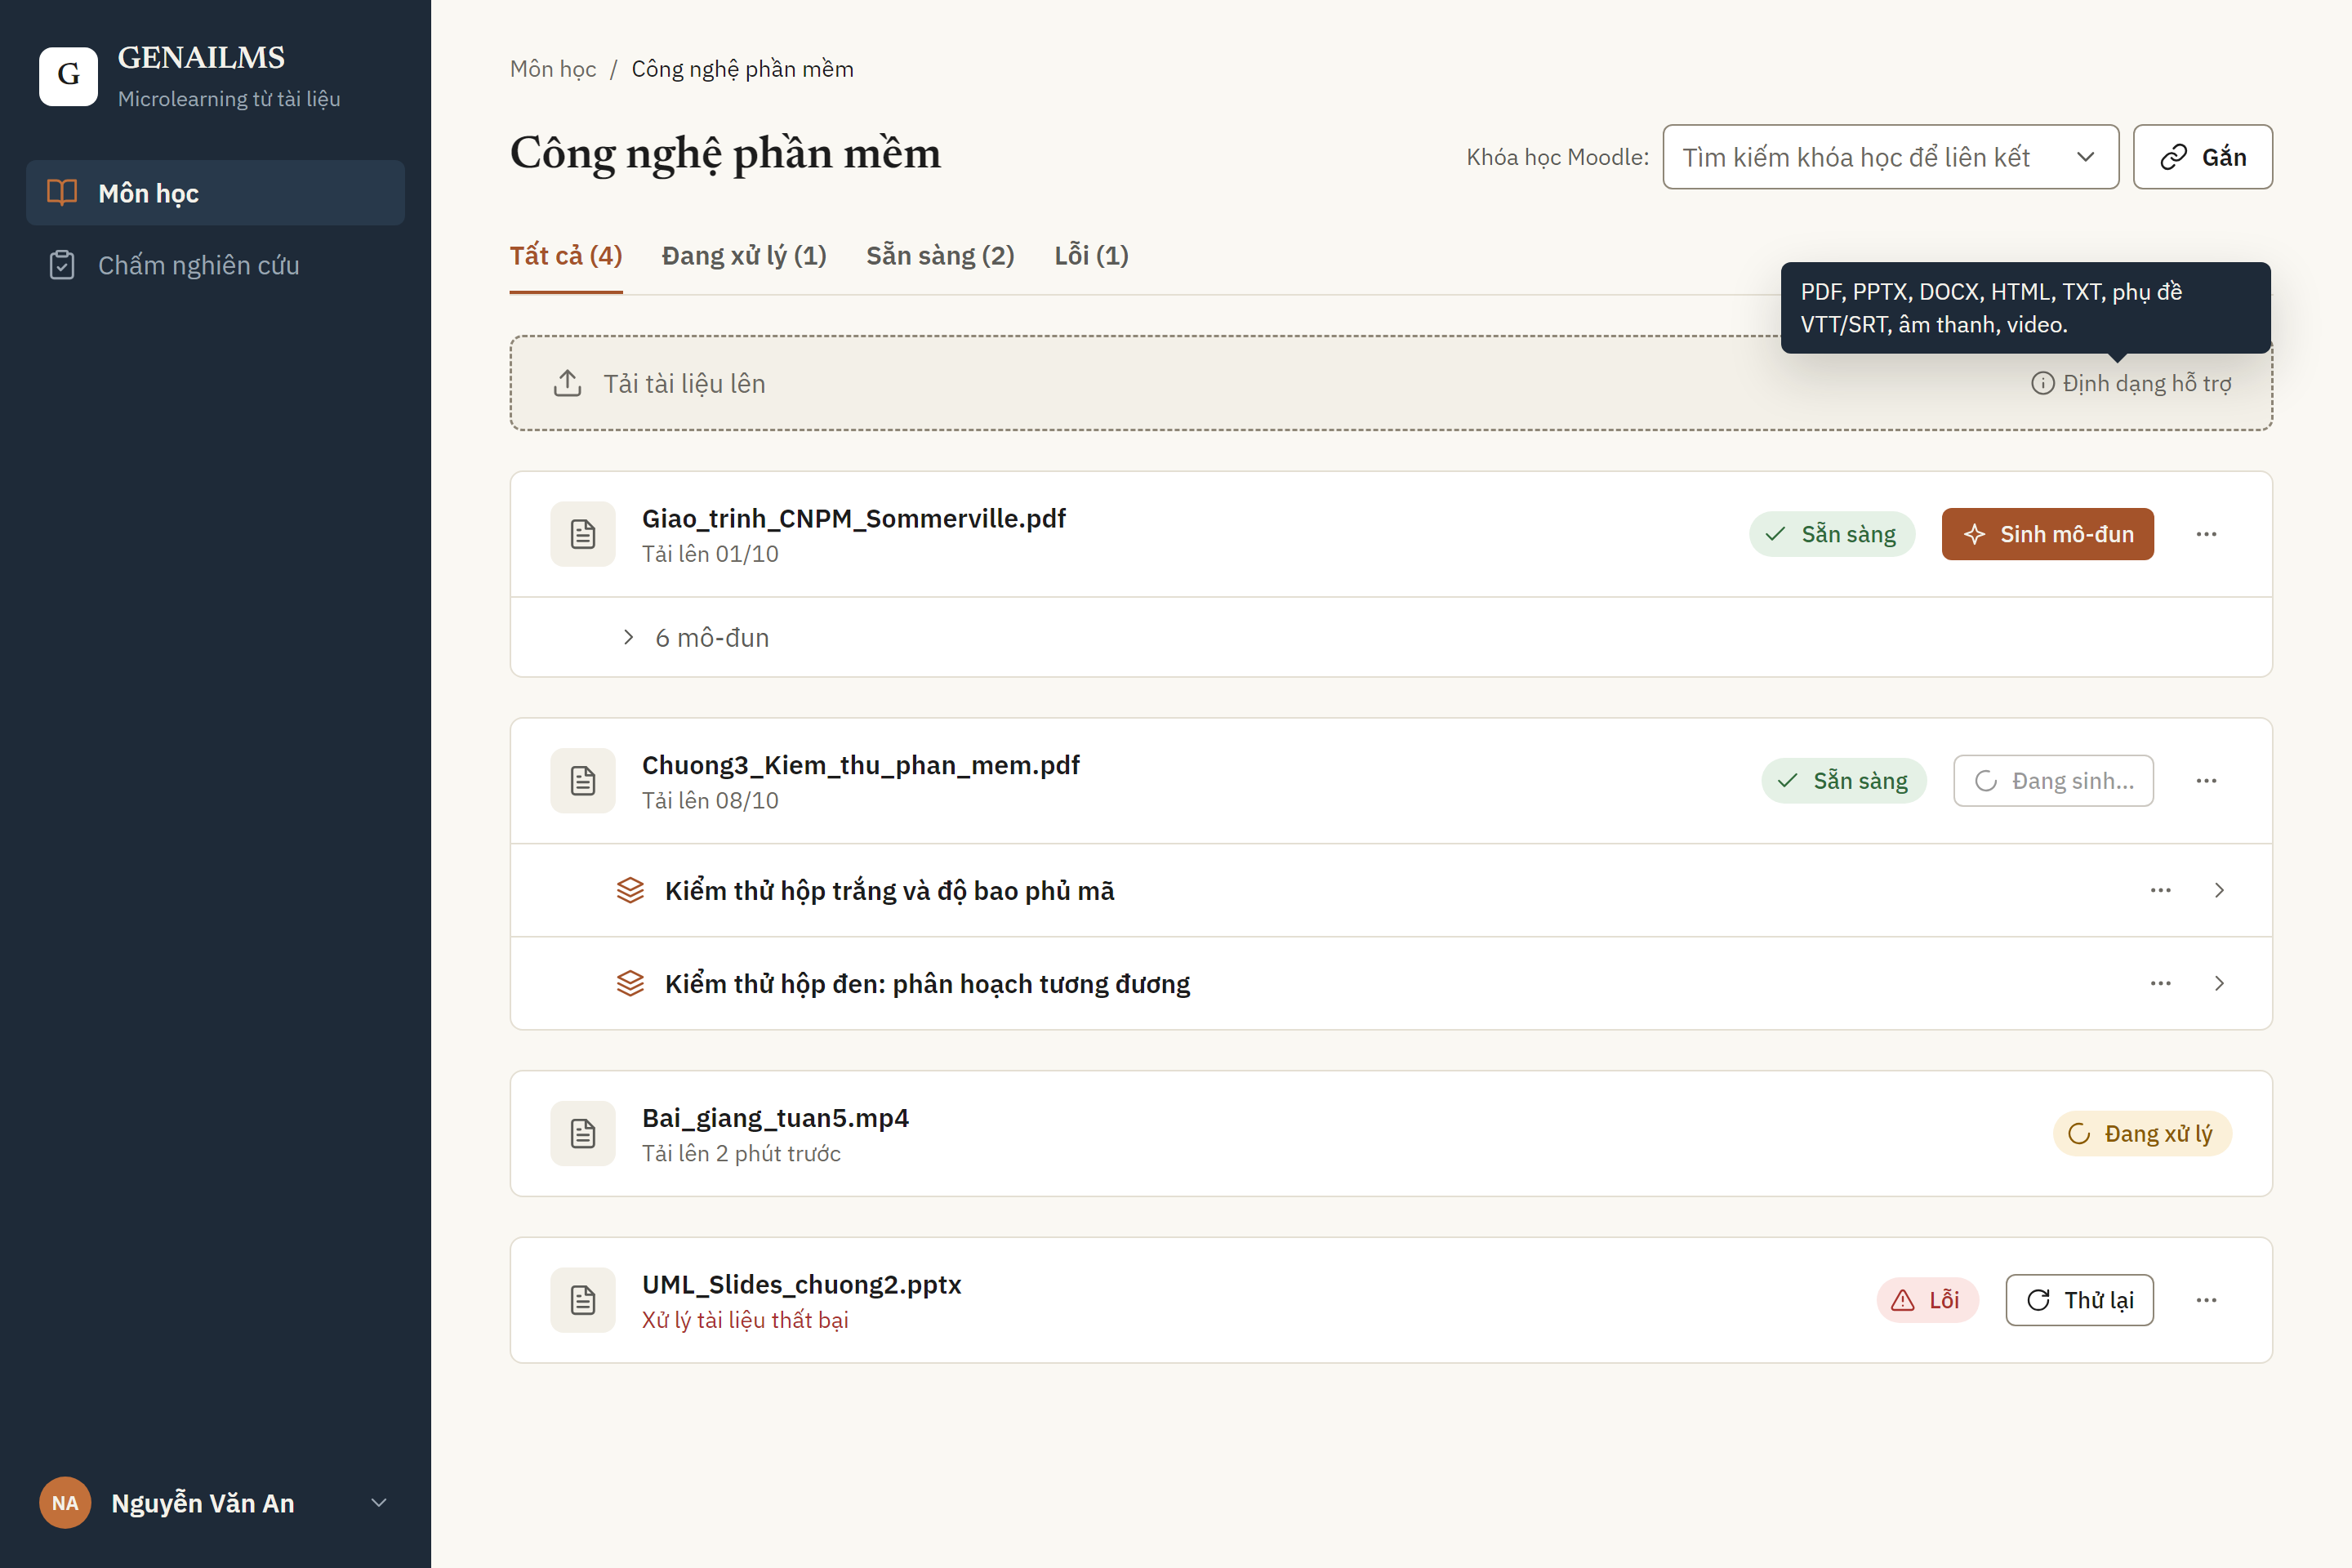
\includegraphics[width=\linewidth,height=.34\textheight,keepaspectratio,viewport={590 600 2820 1800},clip]{graphics/ui/04-course-detail.png}
\caption{Course documents and processing feedback.}\label{fig:ui-screen-04}
\end{figure}

\needspace{.42\textheight}
Figure~\ref{fig:ui-screen-05} asks the author to confirm a model, output language and additional guidance before generation. ``Mặc định'' means ``Default'' and ``Sinh mô-đun'' means ``Generate module''; the saved preference preselects the model without preventing a one-request override.
\begin{figure}[H]\centering
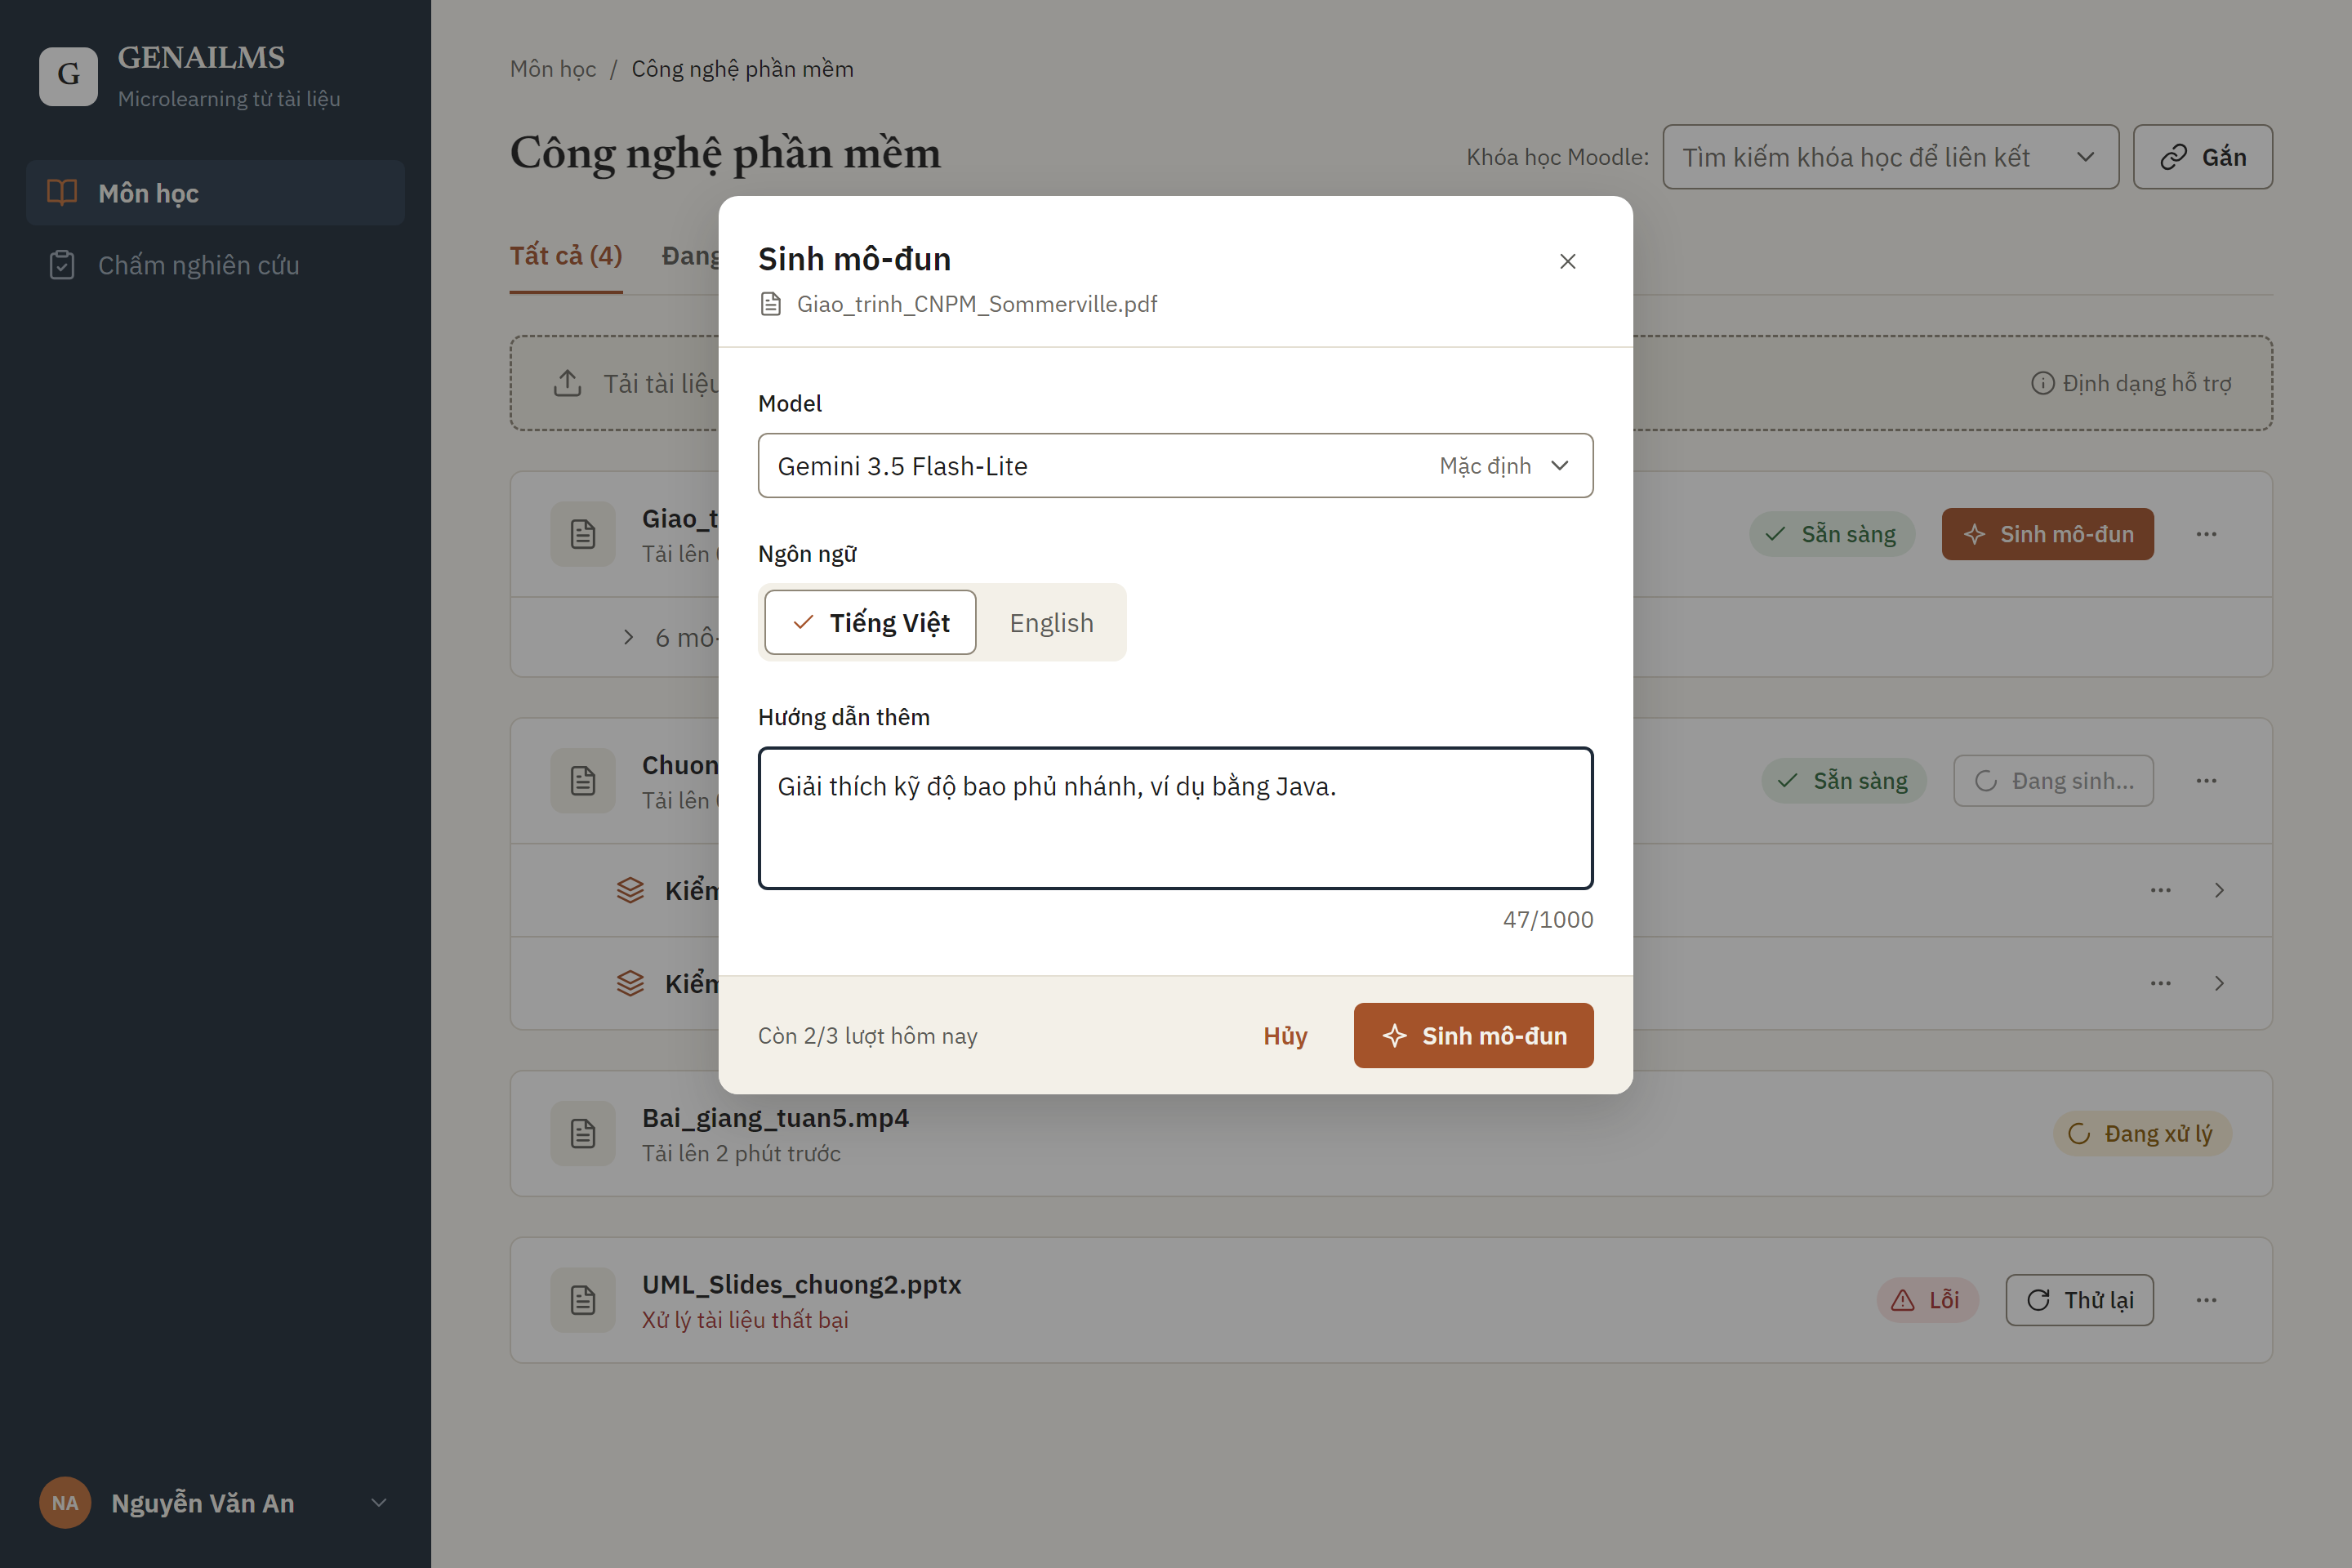
\includegraphics[width=\linewidth,height=.42\textheight,keepaspectratio,viewport={900 585 1980 1510},clip]{graphics/ui/05-generate-module-dialog.png}
\caption{Generation choices before submitting a job.}\label{fig:ui-screen-05}
\end{figure}

\needspace{.42\textheight}
Figure~\ref{fig:ui-screen-06} enlarges the highlighted claim and its source panel as two views of the same screen. ``Nguồn'' means ``Sources'' and ``Khớp'' means ``Matched''; an unresolved source remains visible for review rather than receiving a fabricated match.
\begin{figure}[H]\centering
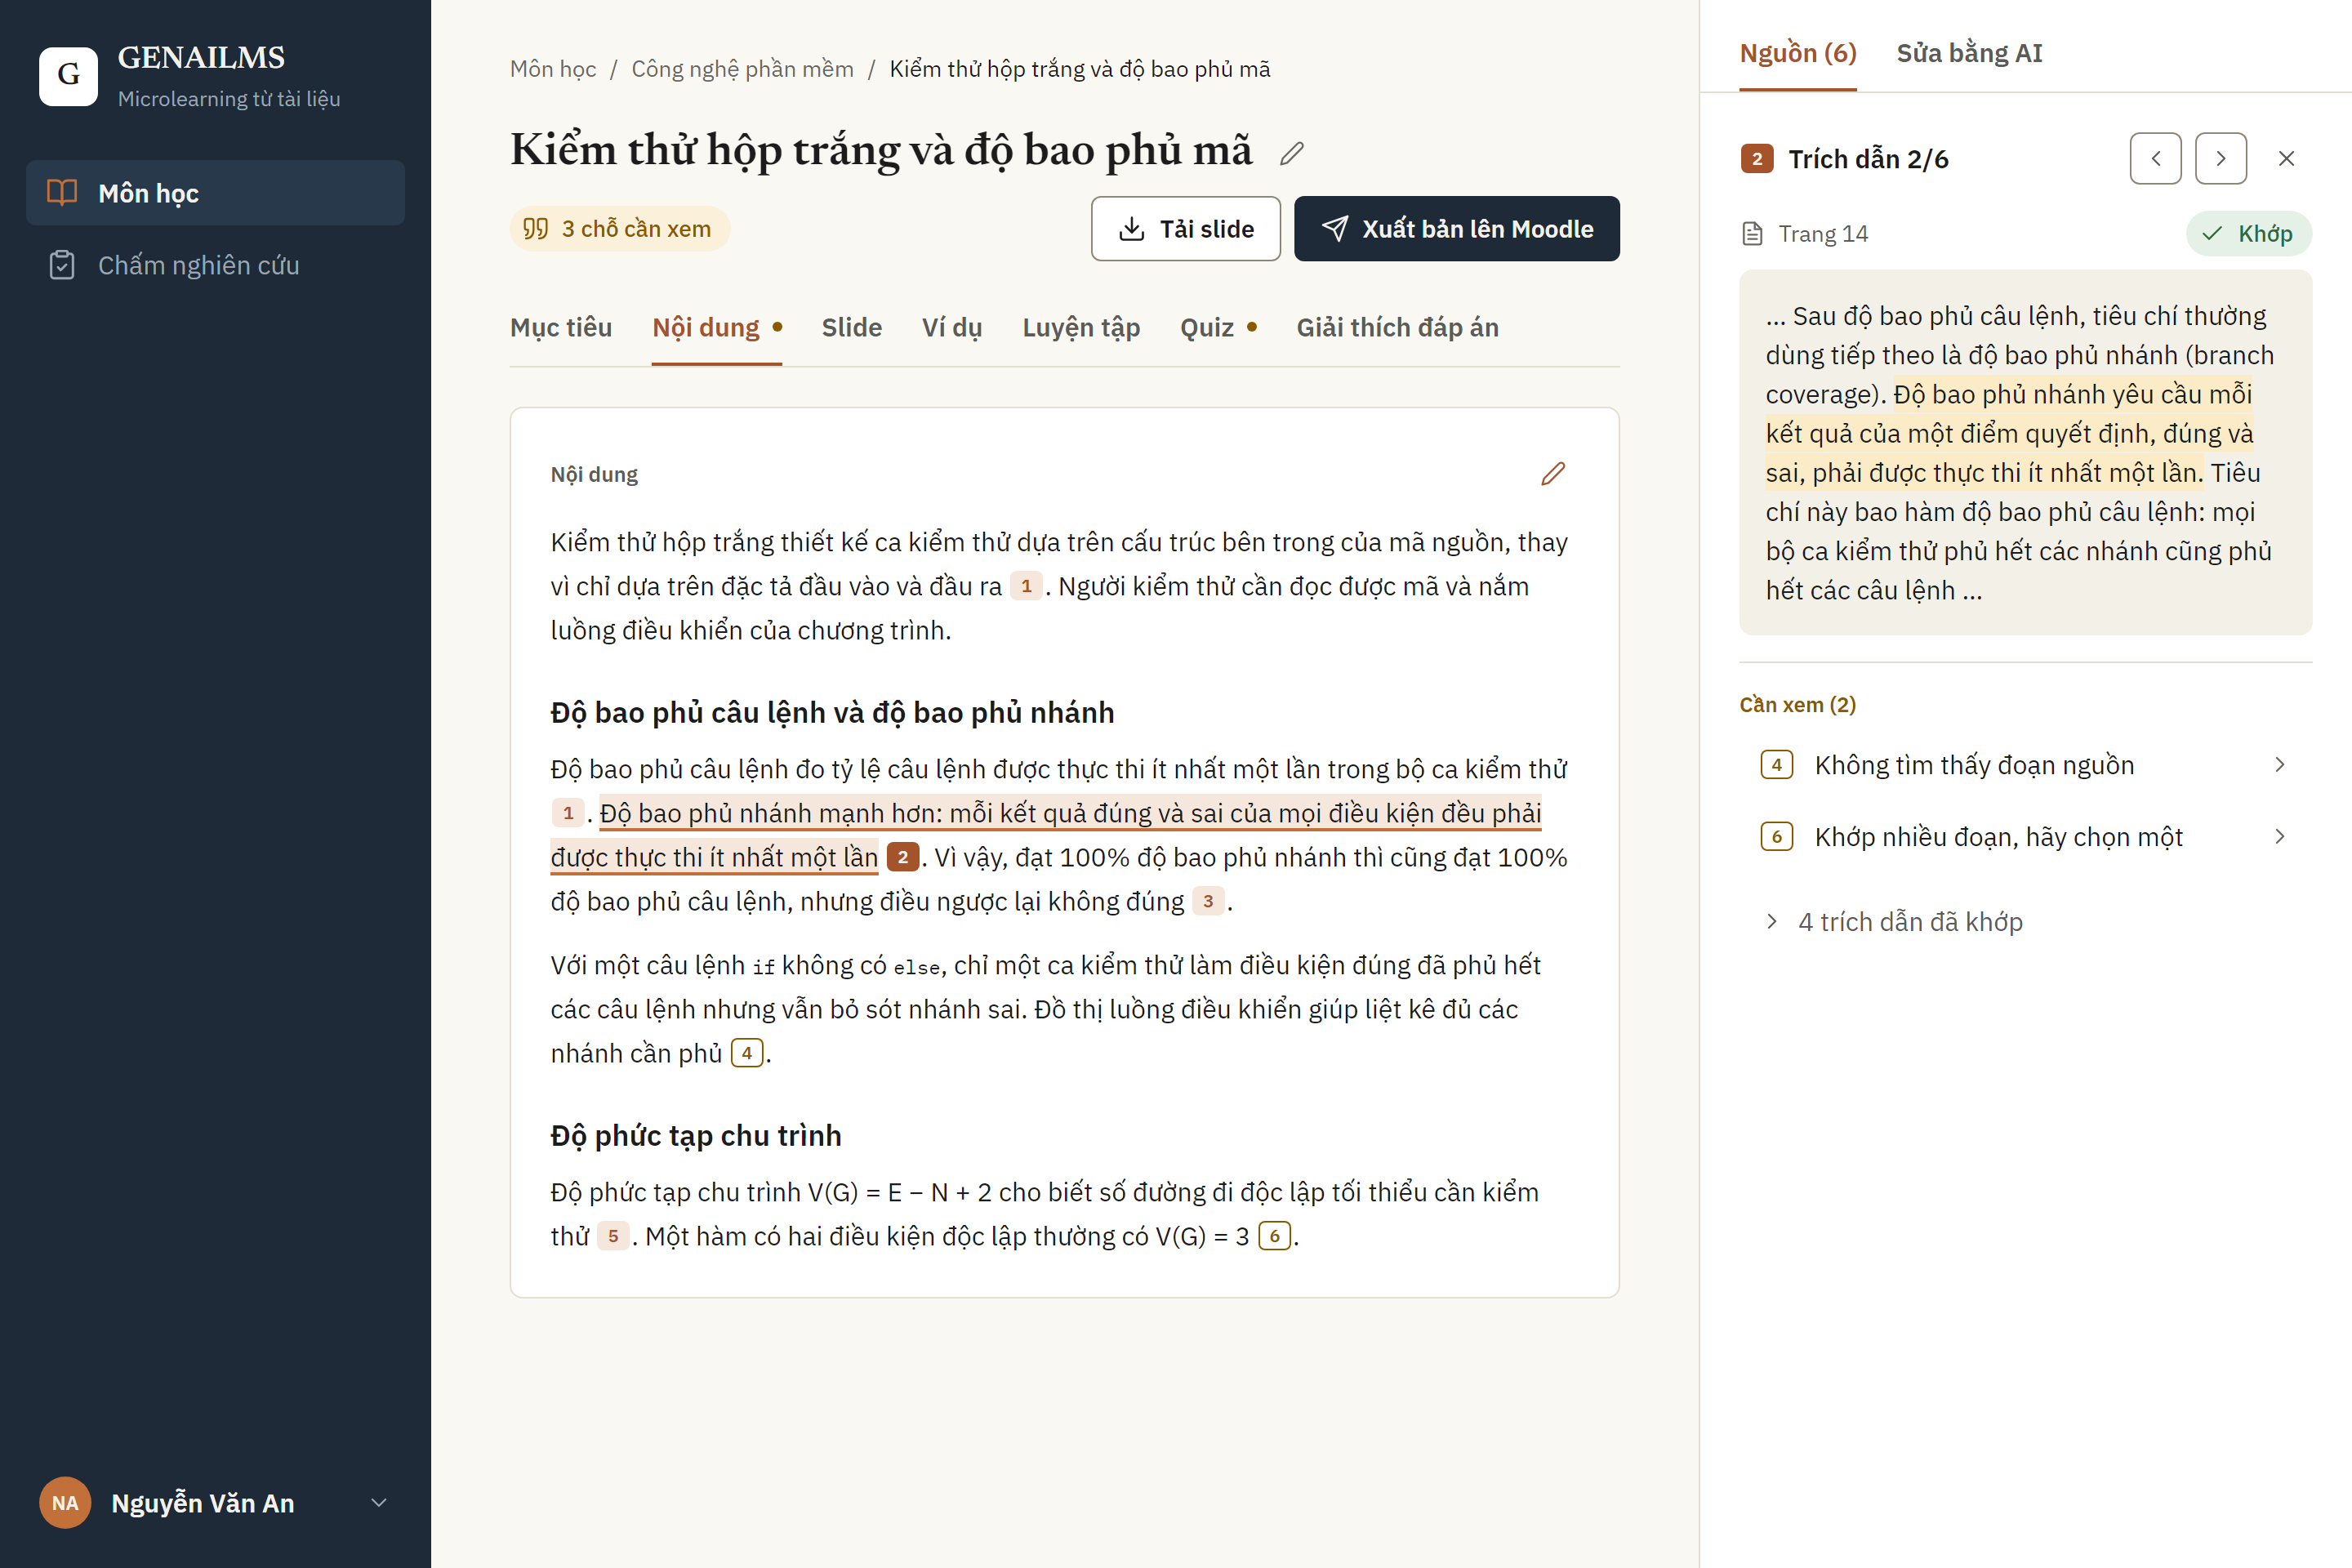
\includegraphics[width=\linewidth,height=.27\textheight,keepaspectratio,viewport={650 570 2000 1150},clip]{graphics/ui/06-module-editor-citations.png}\par\smallskip
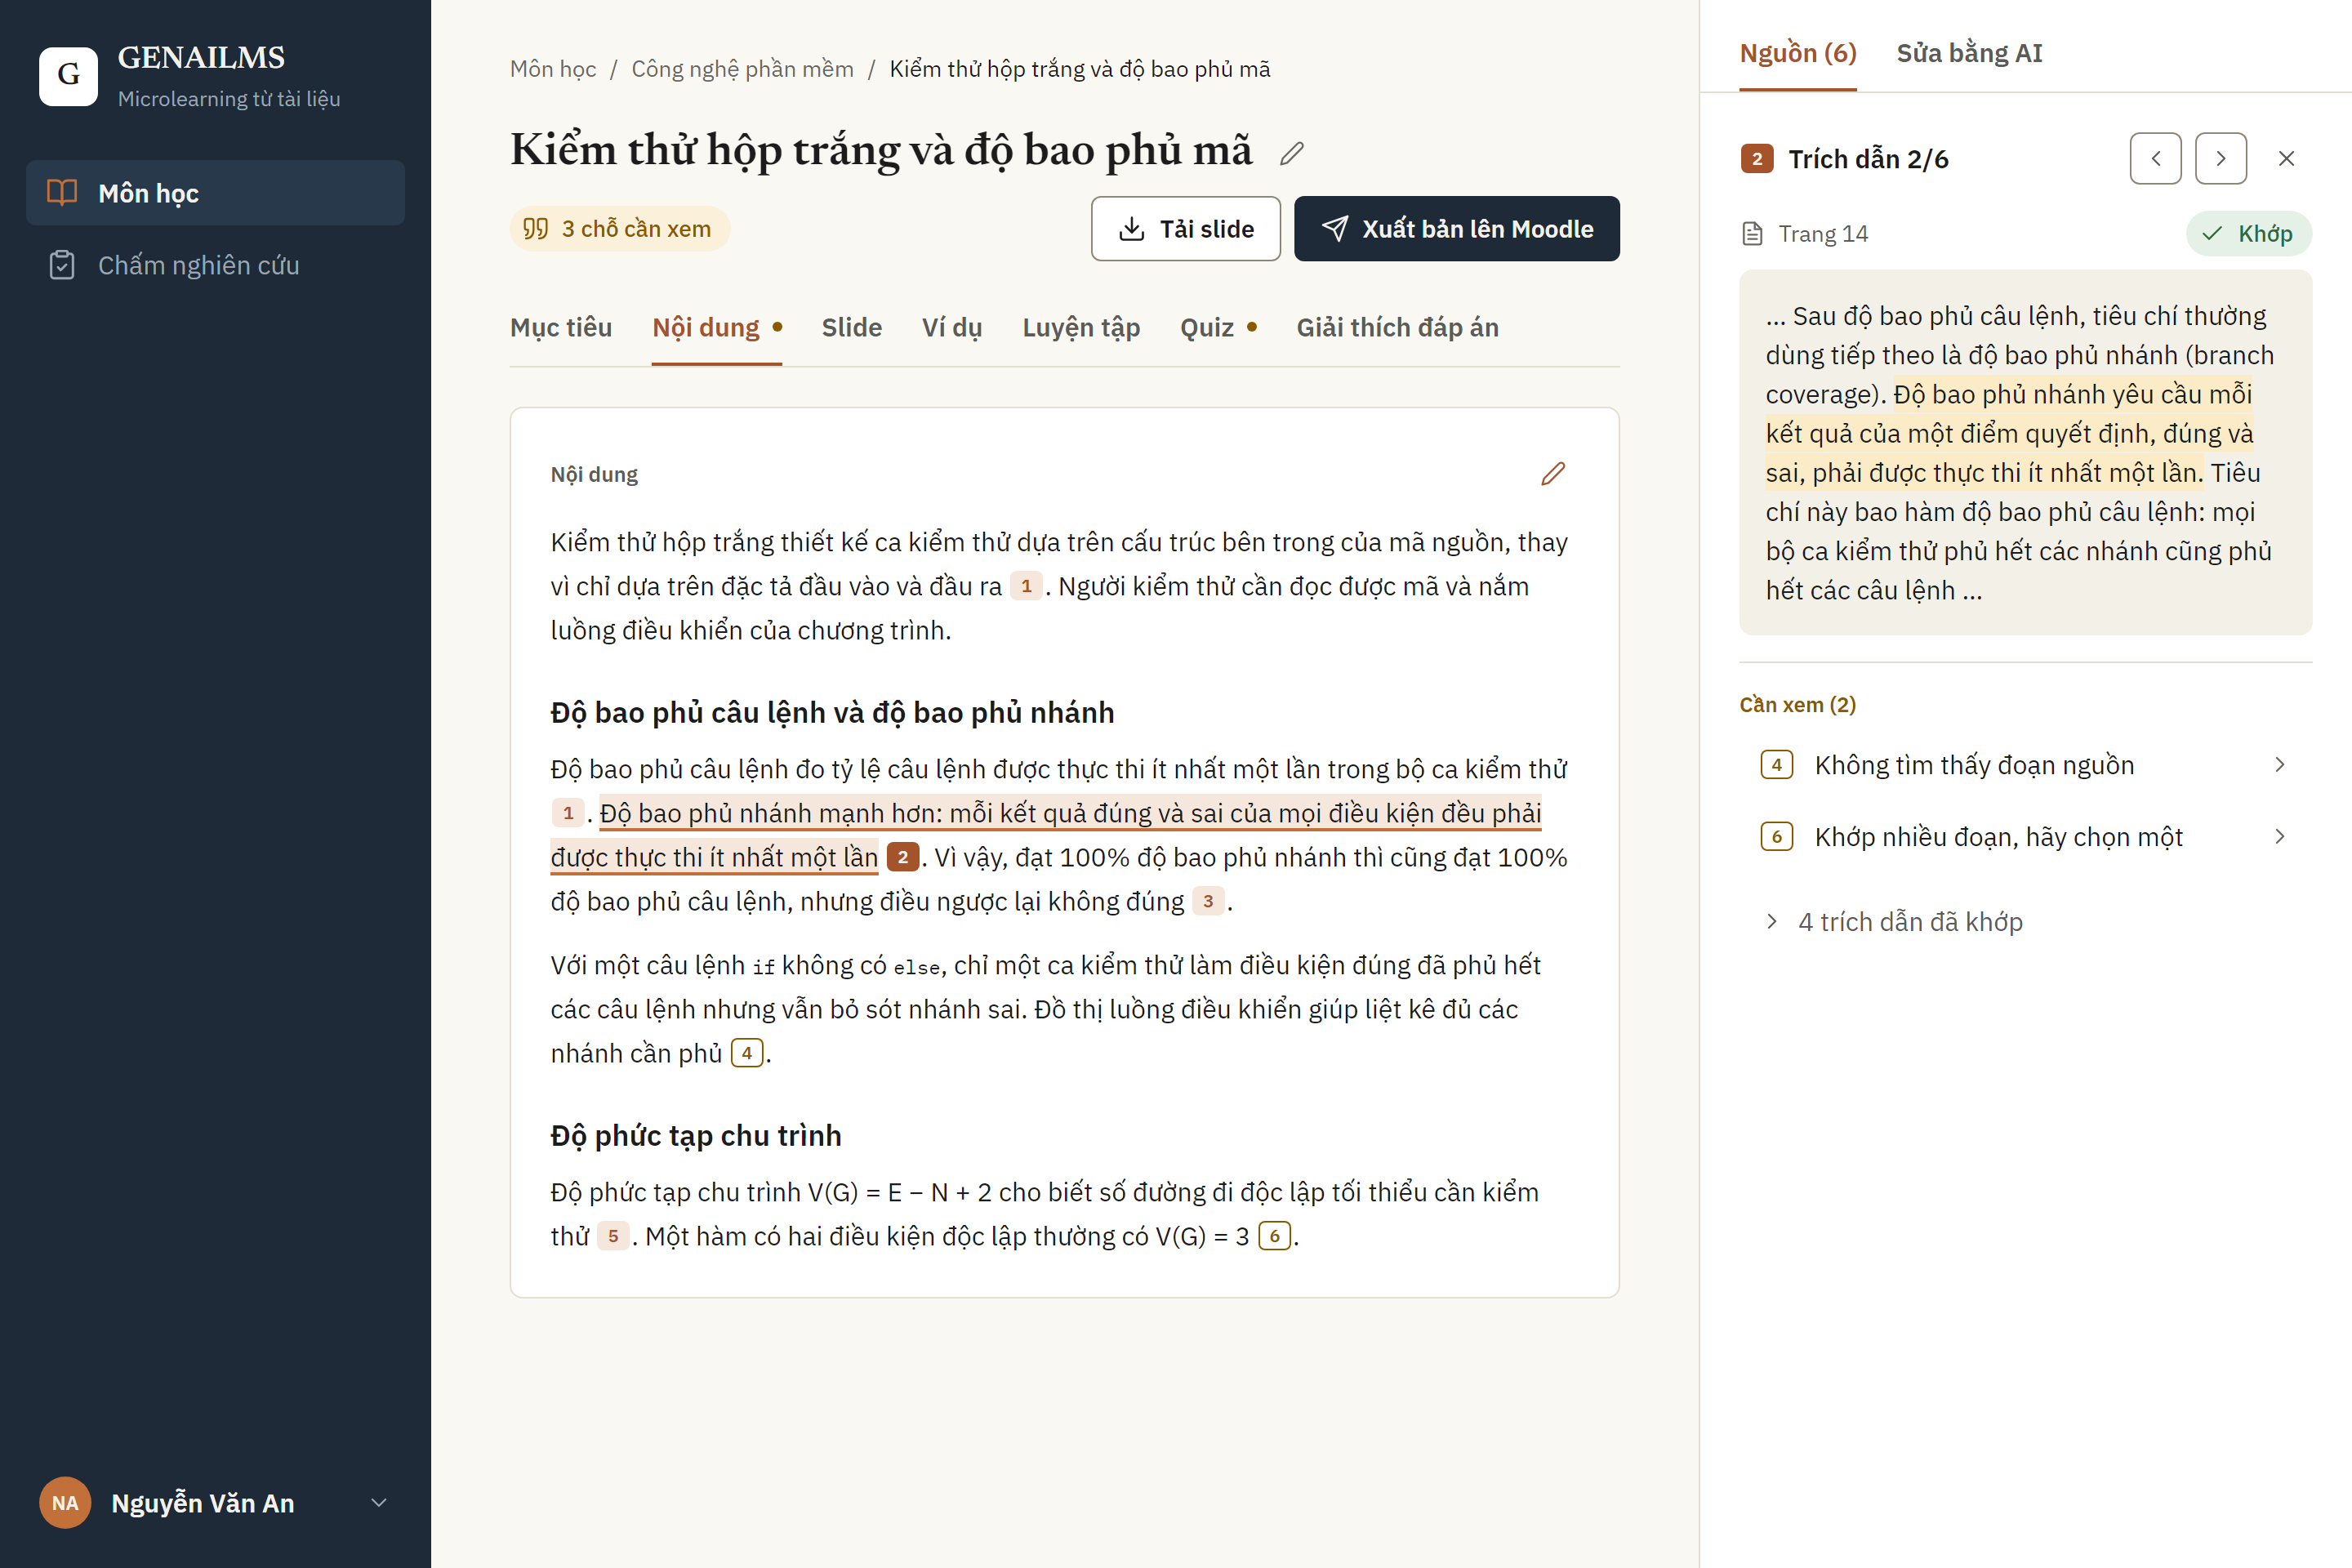
\includegraphics[width=\linewidth,height=.27\textheight,keepaspectratio,viewport={2080 1120 2850 1800},clip]{graphics/ui/06-module-editor-citations.png}
\caption{Claim marker and corresponding physical source passage.}\label{fig:ui-screen-06}
\end{figure}

\needspace{.42\textheight}
The contextual panel in Figure~\ref{fig:ui-screen-07} accepts a component-edit request while retaining the lesson context. ``Sửa bằng AI'' means ``Edit with AI''; accepting an edit follows the same validation and original-preservation contract as a manual change.
\begin{figure}[H]\centering
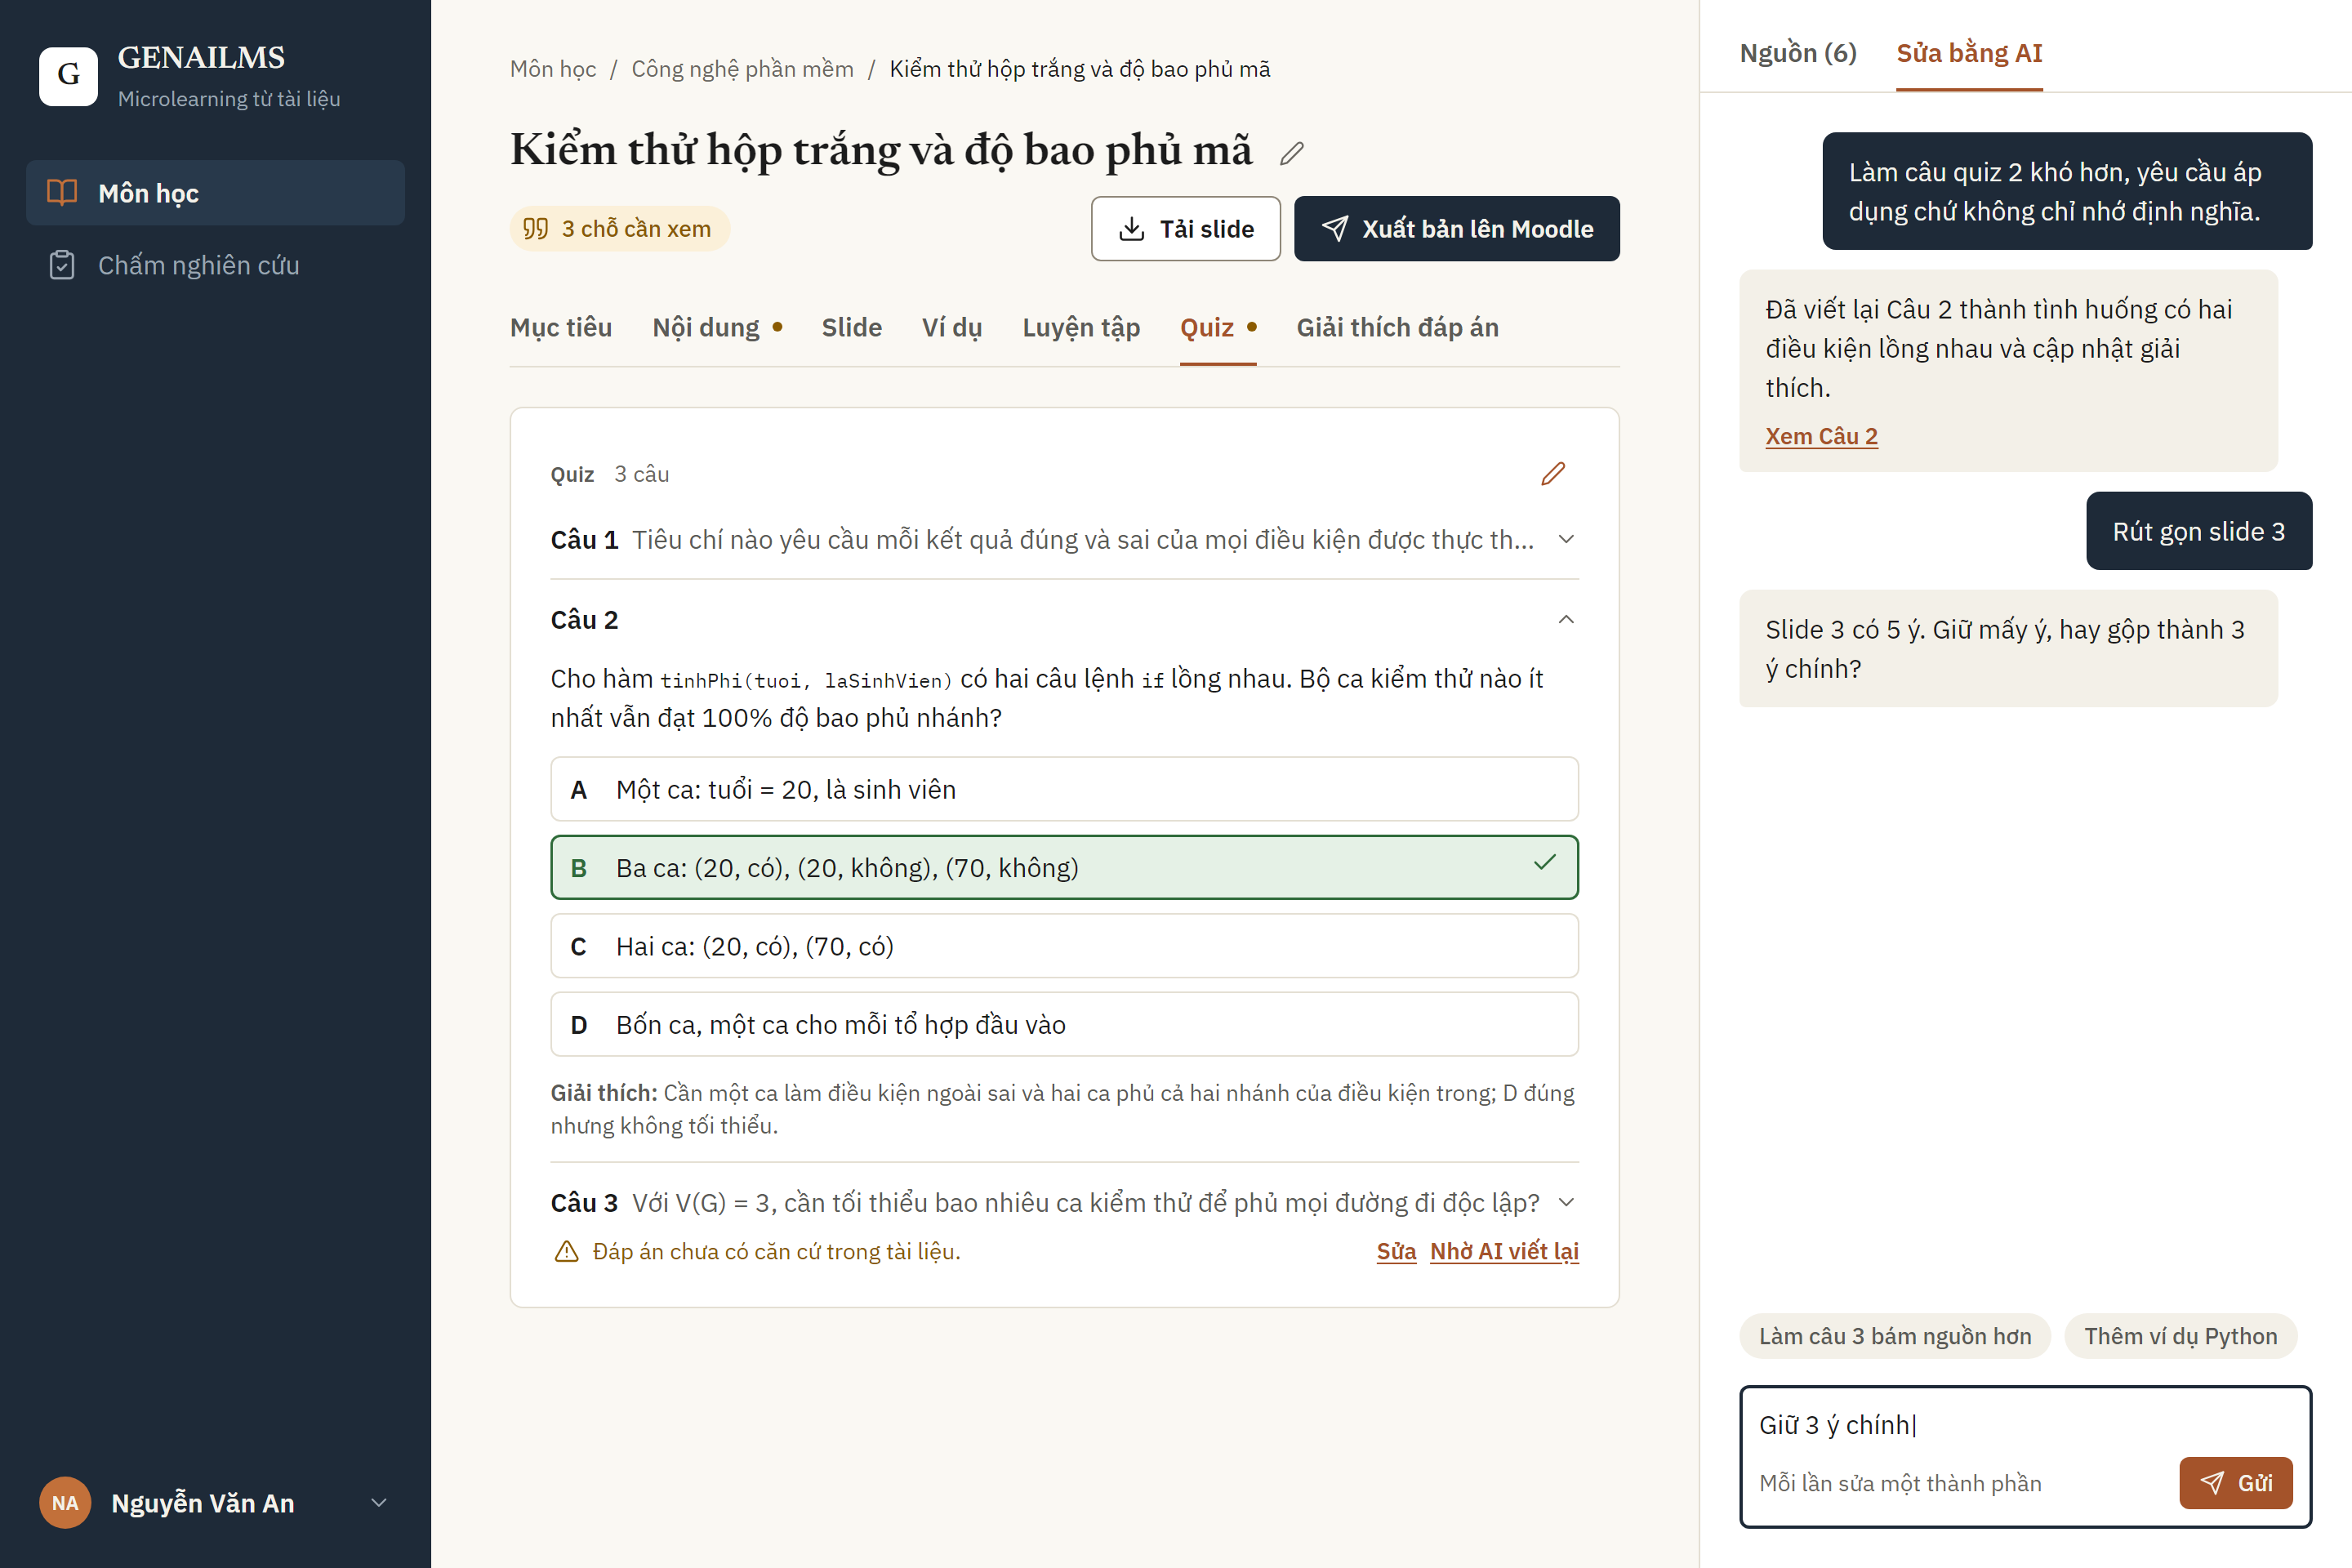
\includegraphics[width=\linewidth,height=.34\textheight,keepaspectratio,viewport={2100 1320 2850 1780},clip]{graphics/ui/07-module-editor-chat-edit.png}
\caption{Contextual editing request and response.}\label{fig:ui-screen-07}
\end{figure}

\needspace{.42\textheight}
Figure~\ref{fig:ui-screen-08} makes the target course/section and activity selection visible before publication. ``Xuất bản lên Moodle'' means ``Publish to Moodle''; the explicit confirmation reduces accidental publication to a remembered destination.
\begin{figure}[H]\centering
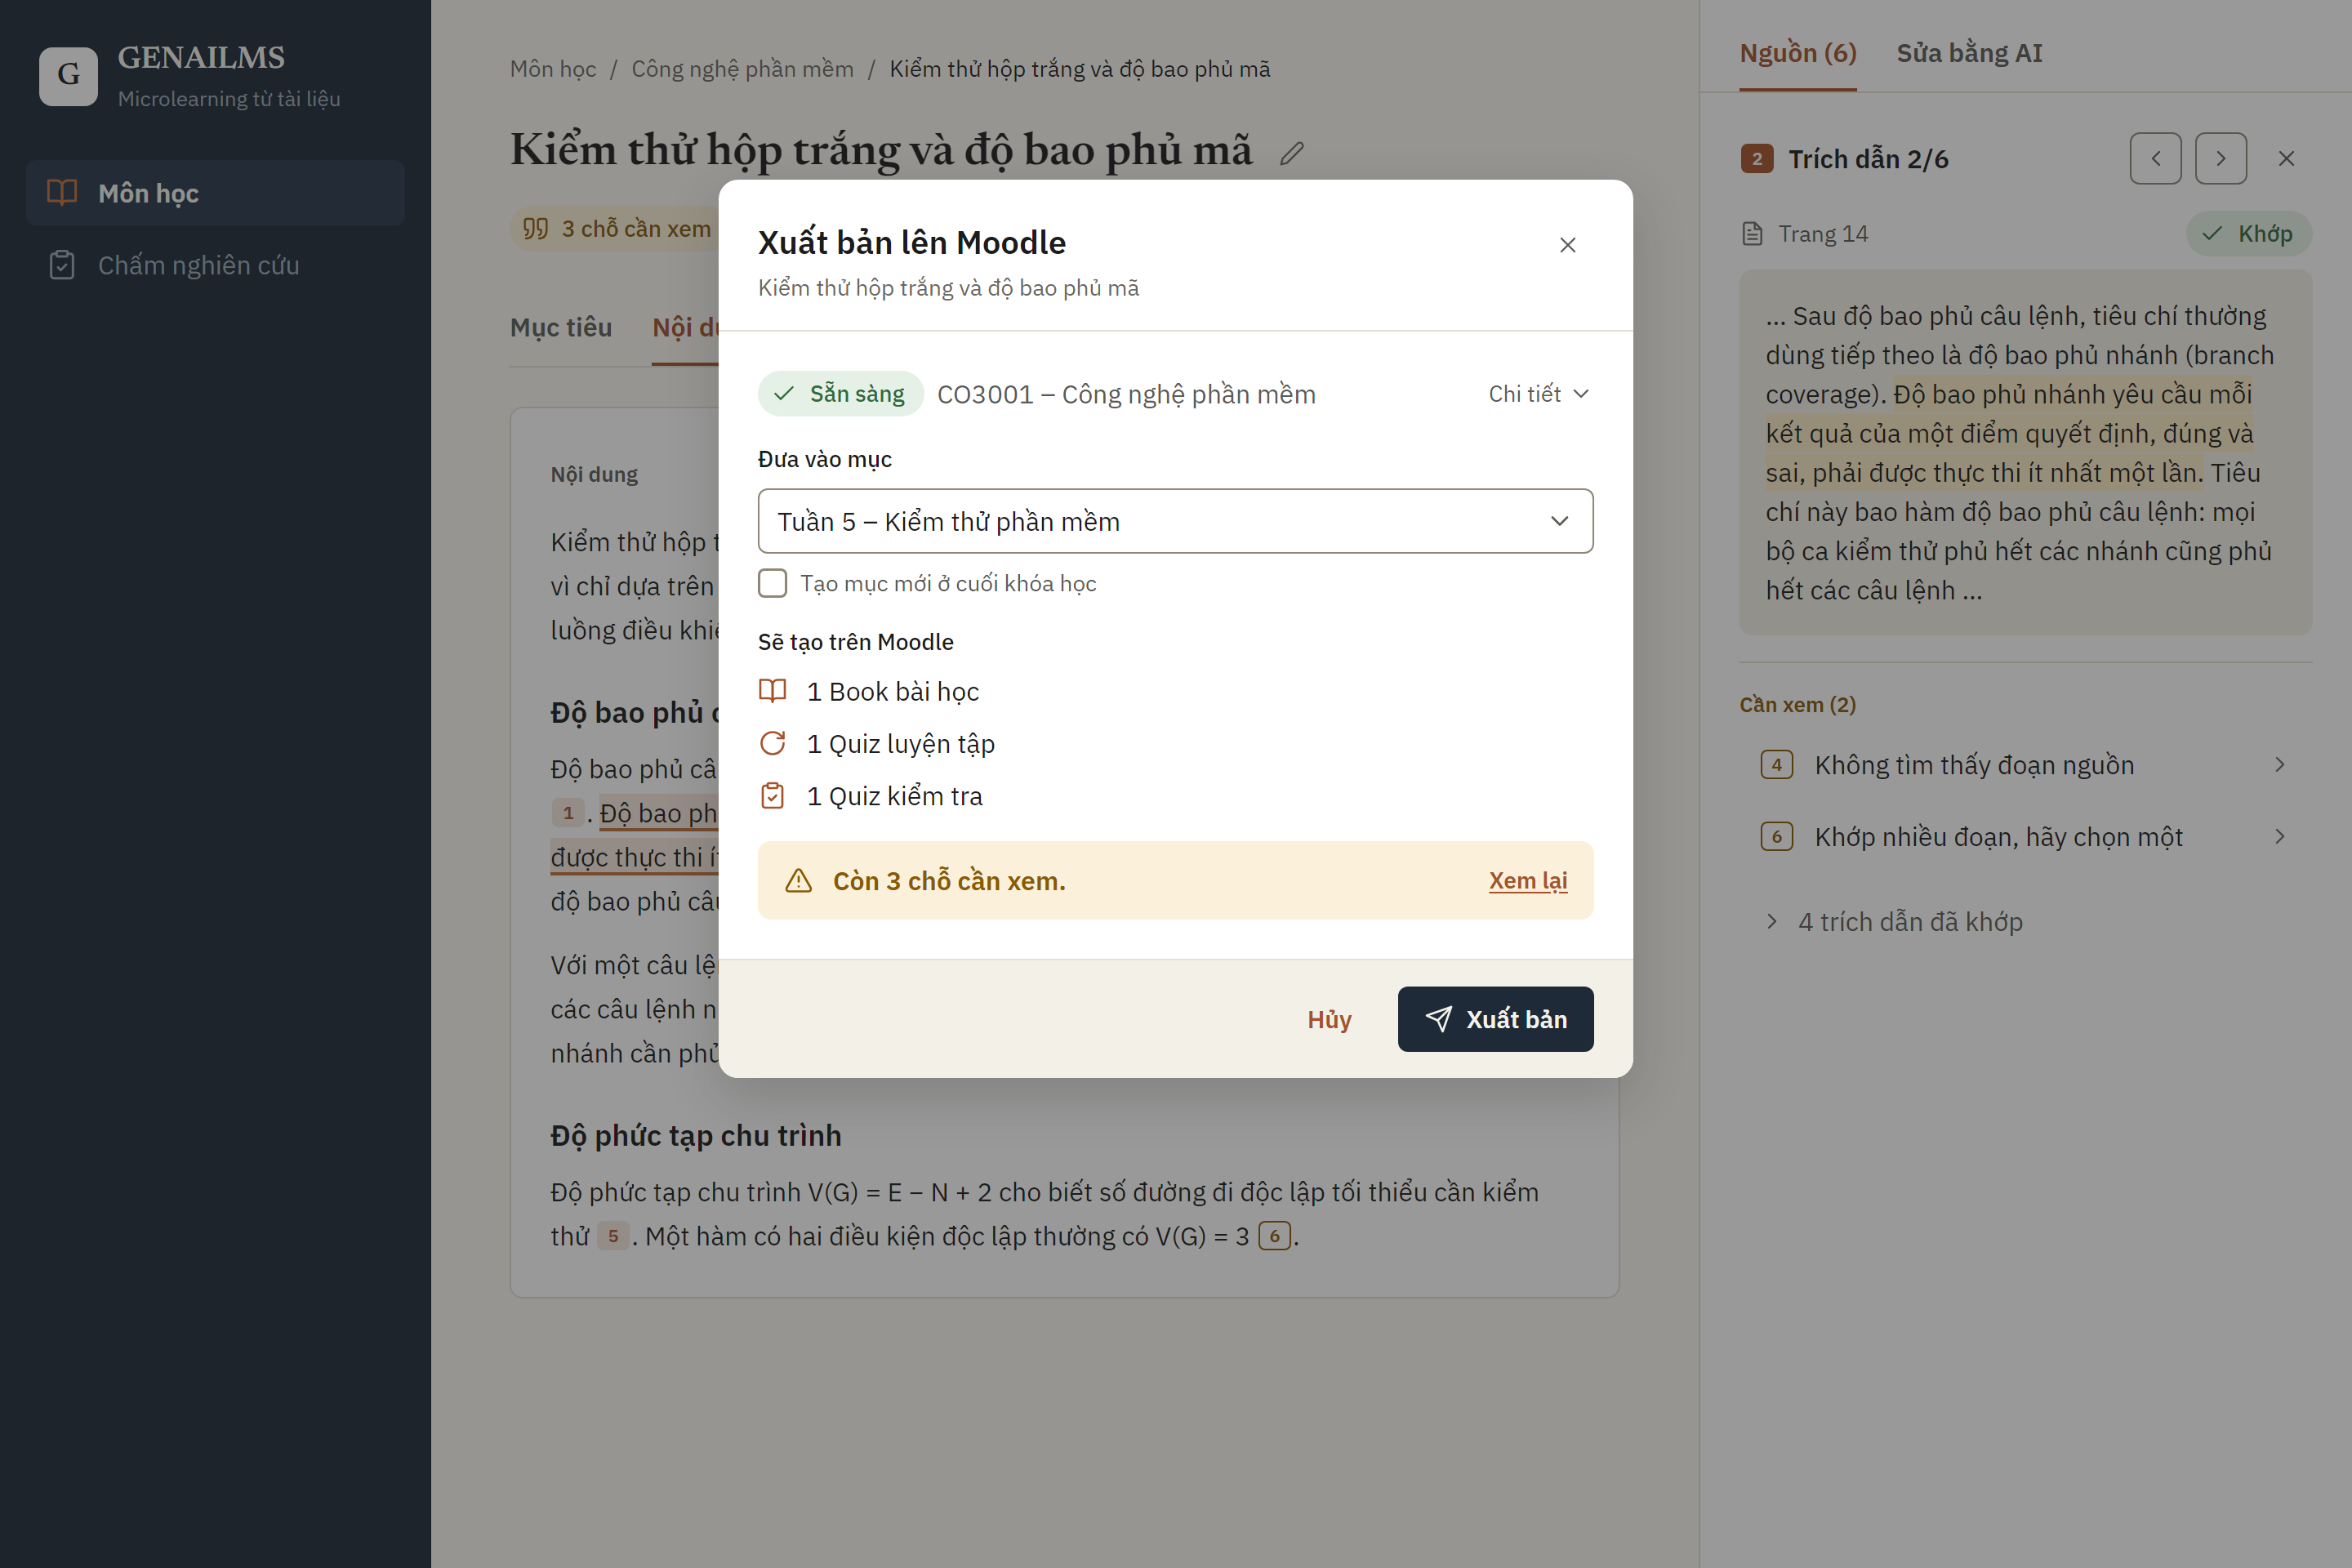
\includegraphics[width=\linewidth,height=.42\textheight,keepaspectratio,viewport={900 600 1980 1510},clip]{graphics/ui/08-publish-to-moodle.png}
\caption{Publication destination and activity review.}\label{fig:ui-screen-08}
\end{figure}

\needspace{.42\textheight}
Figure~\ref{fig:ui-screen-09} highlights pending identity confirmation and its next action. Account linking and course permission remain separate states; subsequent publication verifies the target-course capabilities without exposing account existence through the generic link-request response.
\begin{figure}[H]\centering
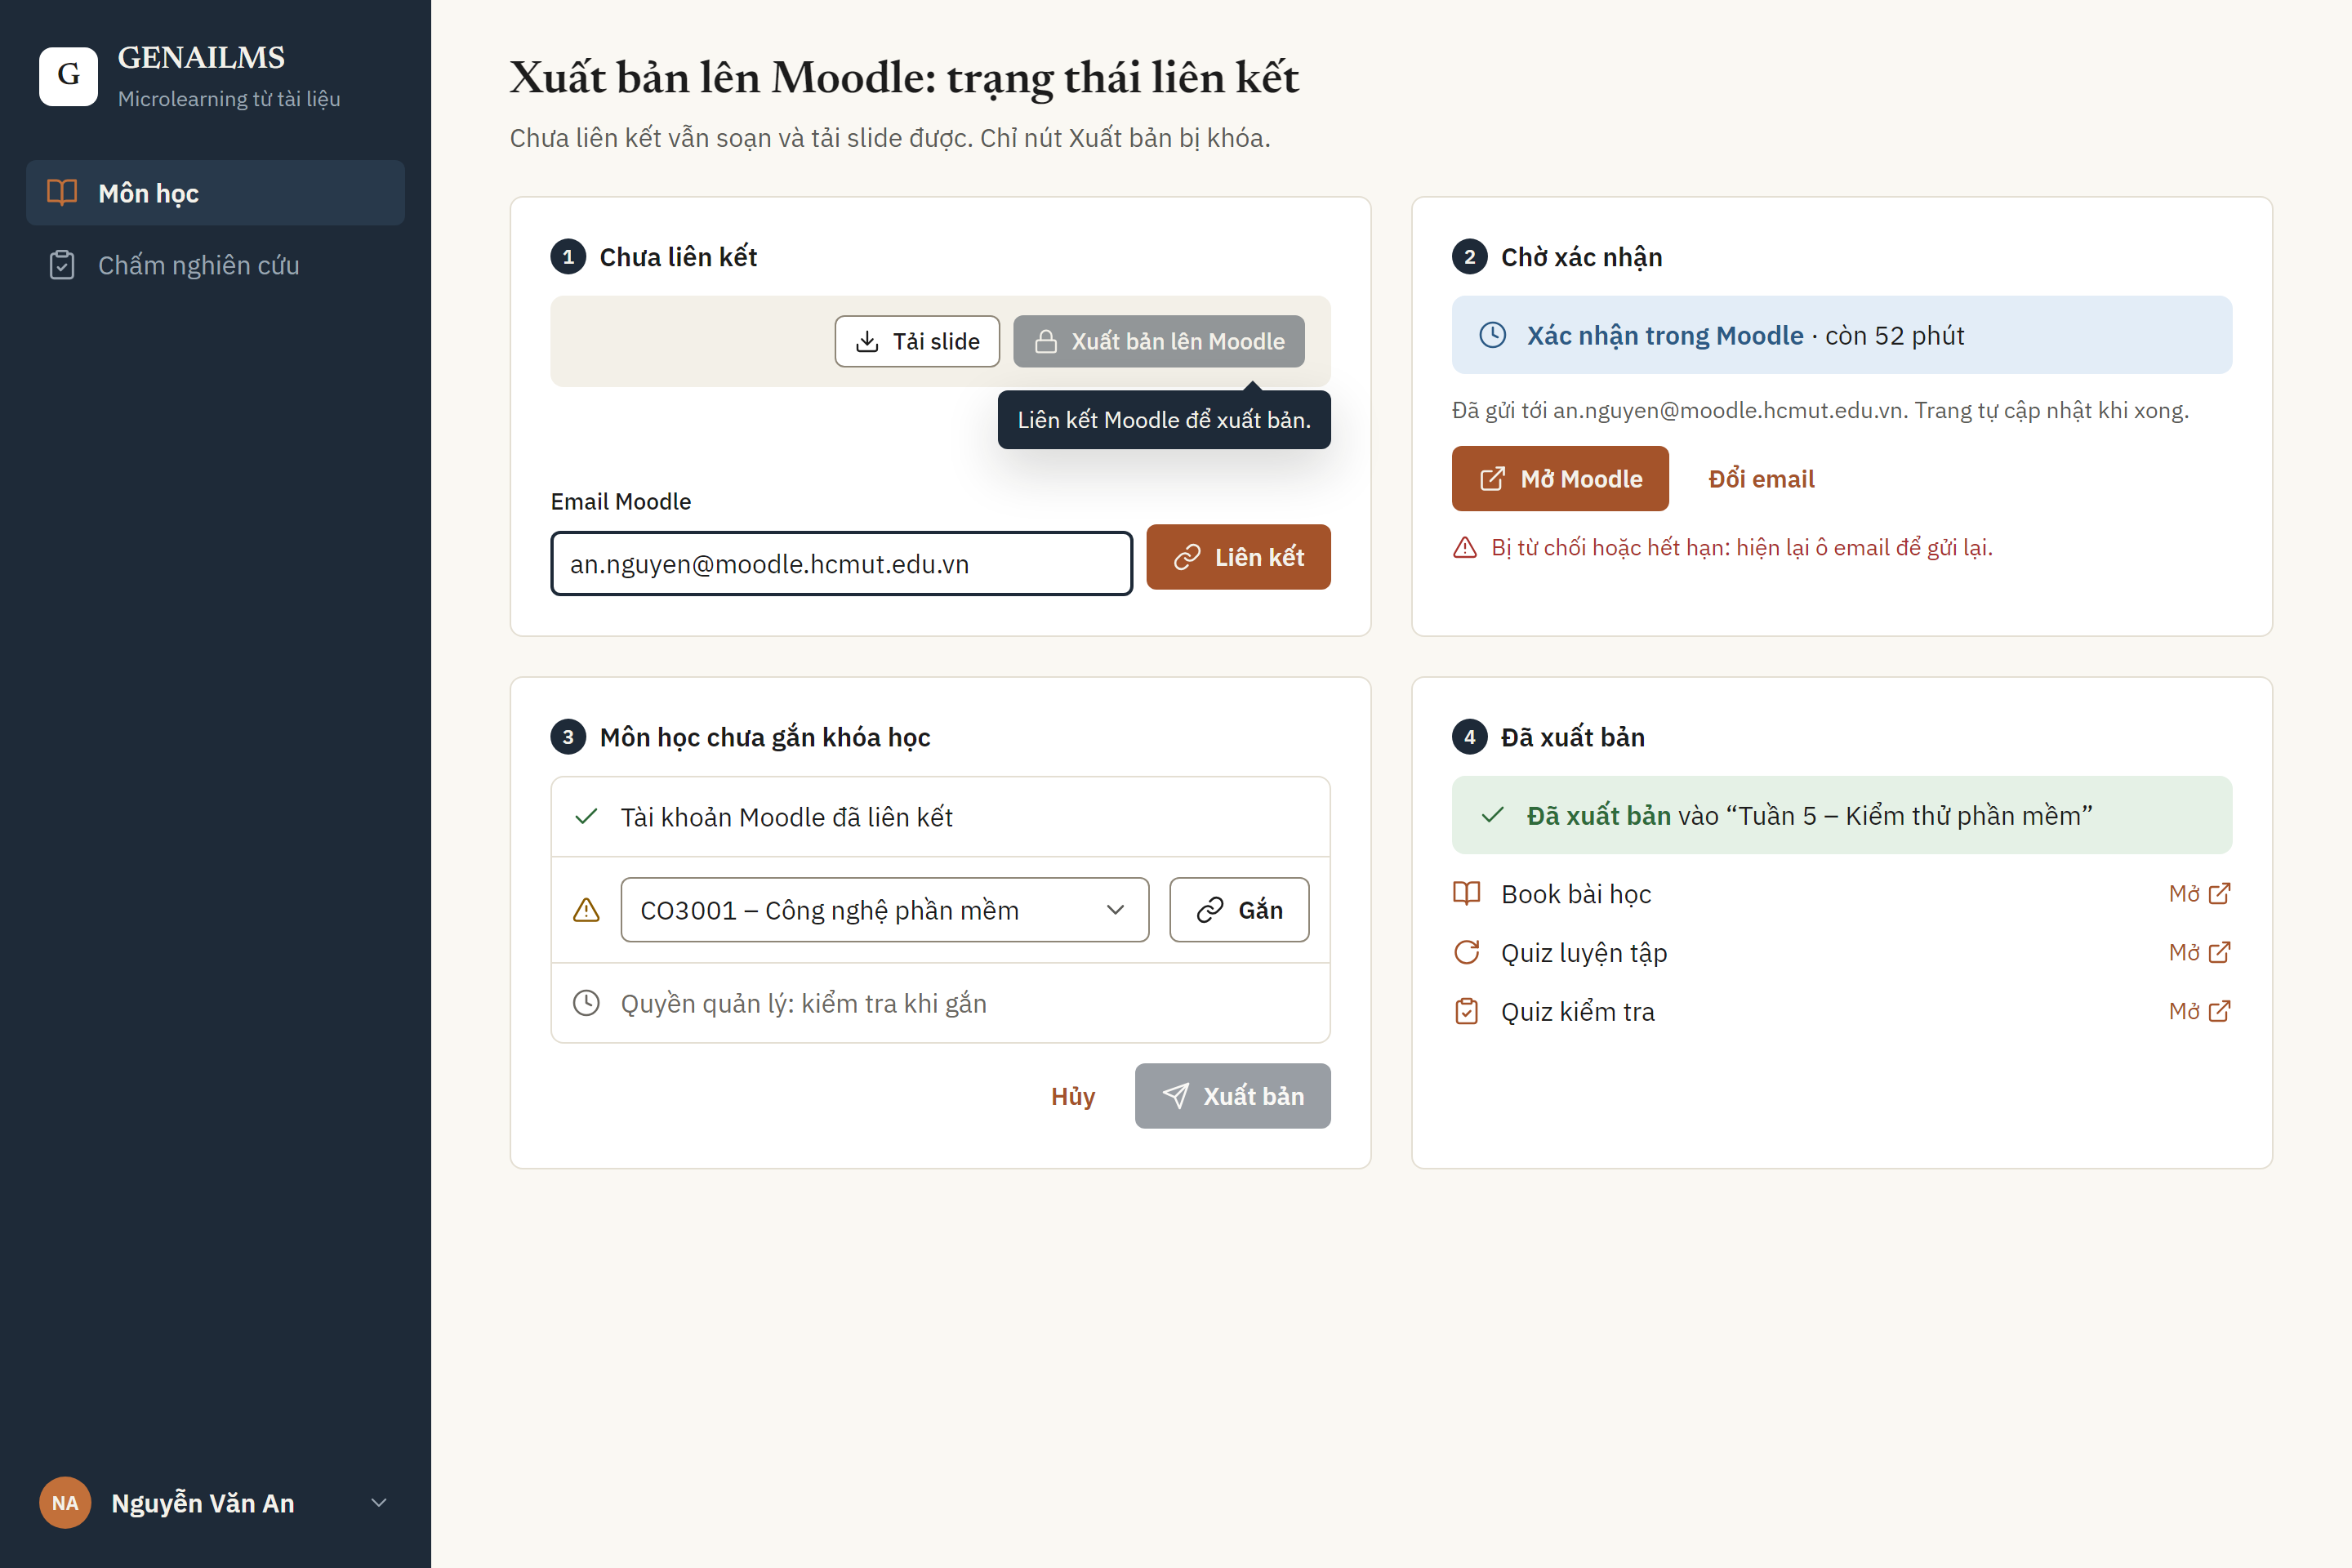
\includegraphics[width=\linewidth,height=.34\textheight,keepaspectratio,viewport={1710 1120 2810 1700},clip]{graphics/ui/09-publish-moodle-link-states.png}
\caption{Pending Moodle confirmation and next actions.}\label{fig:ui-screen-09}
\end{figure}

\needspace{.42\textheight}
The row menu in Figure~\ref{fig:ui-screen-10} groups account actions by the selected person. ``Đặt lại mật khẩu'' means ``Reset password'' and ``Vô hiệu hóa'' means ``Disable''; administrator status does not grant general access to the person's teaching content.
\begin{figure}[H]\centering
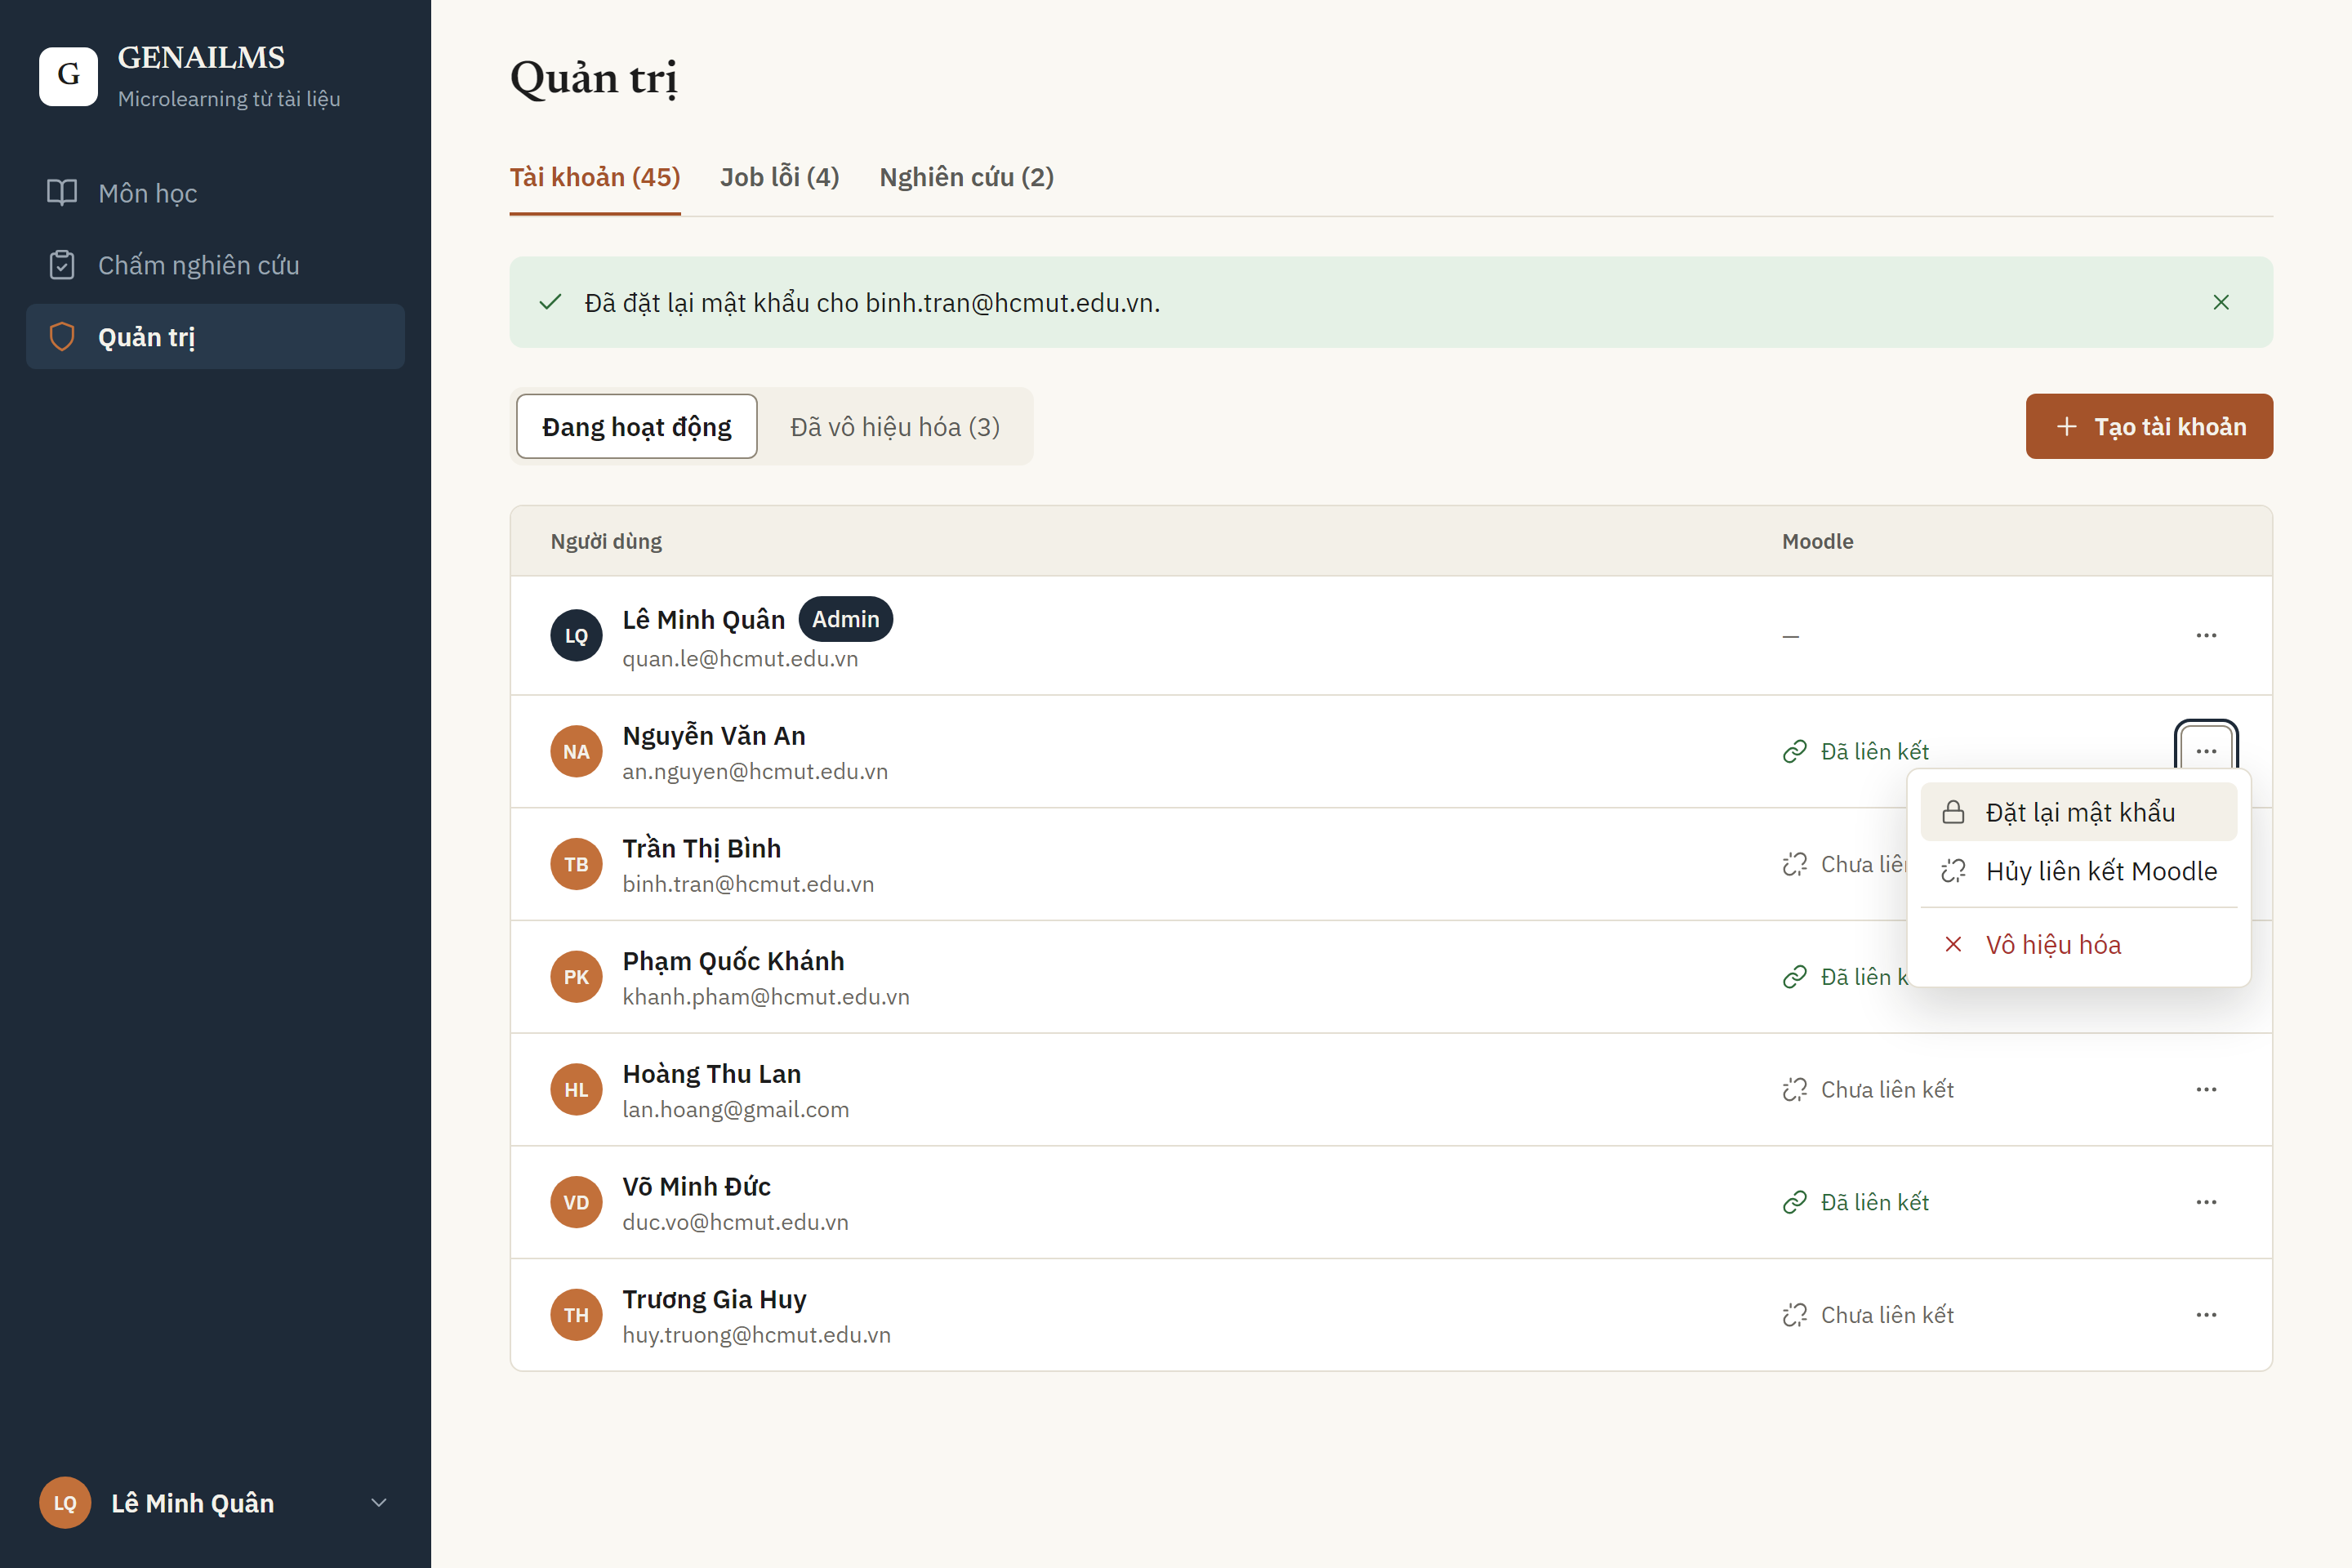
\includegraphics[width=\linewidth,height=.34\textheight,keepaspectratio,viewport={1900 650 2820 1450},clip]{graphics/ui/10-admin-accounts.png}
\caption{Contextual account-administration actions.}\label{fig:ui-screen-10}
\end{figure}

\needspace{.42\textheight}
Figure~\ref{fig:ui-screen-11} exposes failure detail and the permitted retry action. ``Thử lại'' means ``Retry''; the interface distinguishes an author's own job from the administrator's operational recovery scope.
\begin{figure}[H]\centering
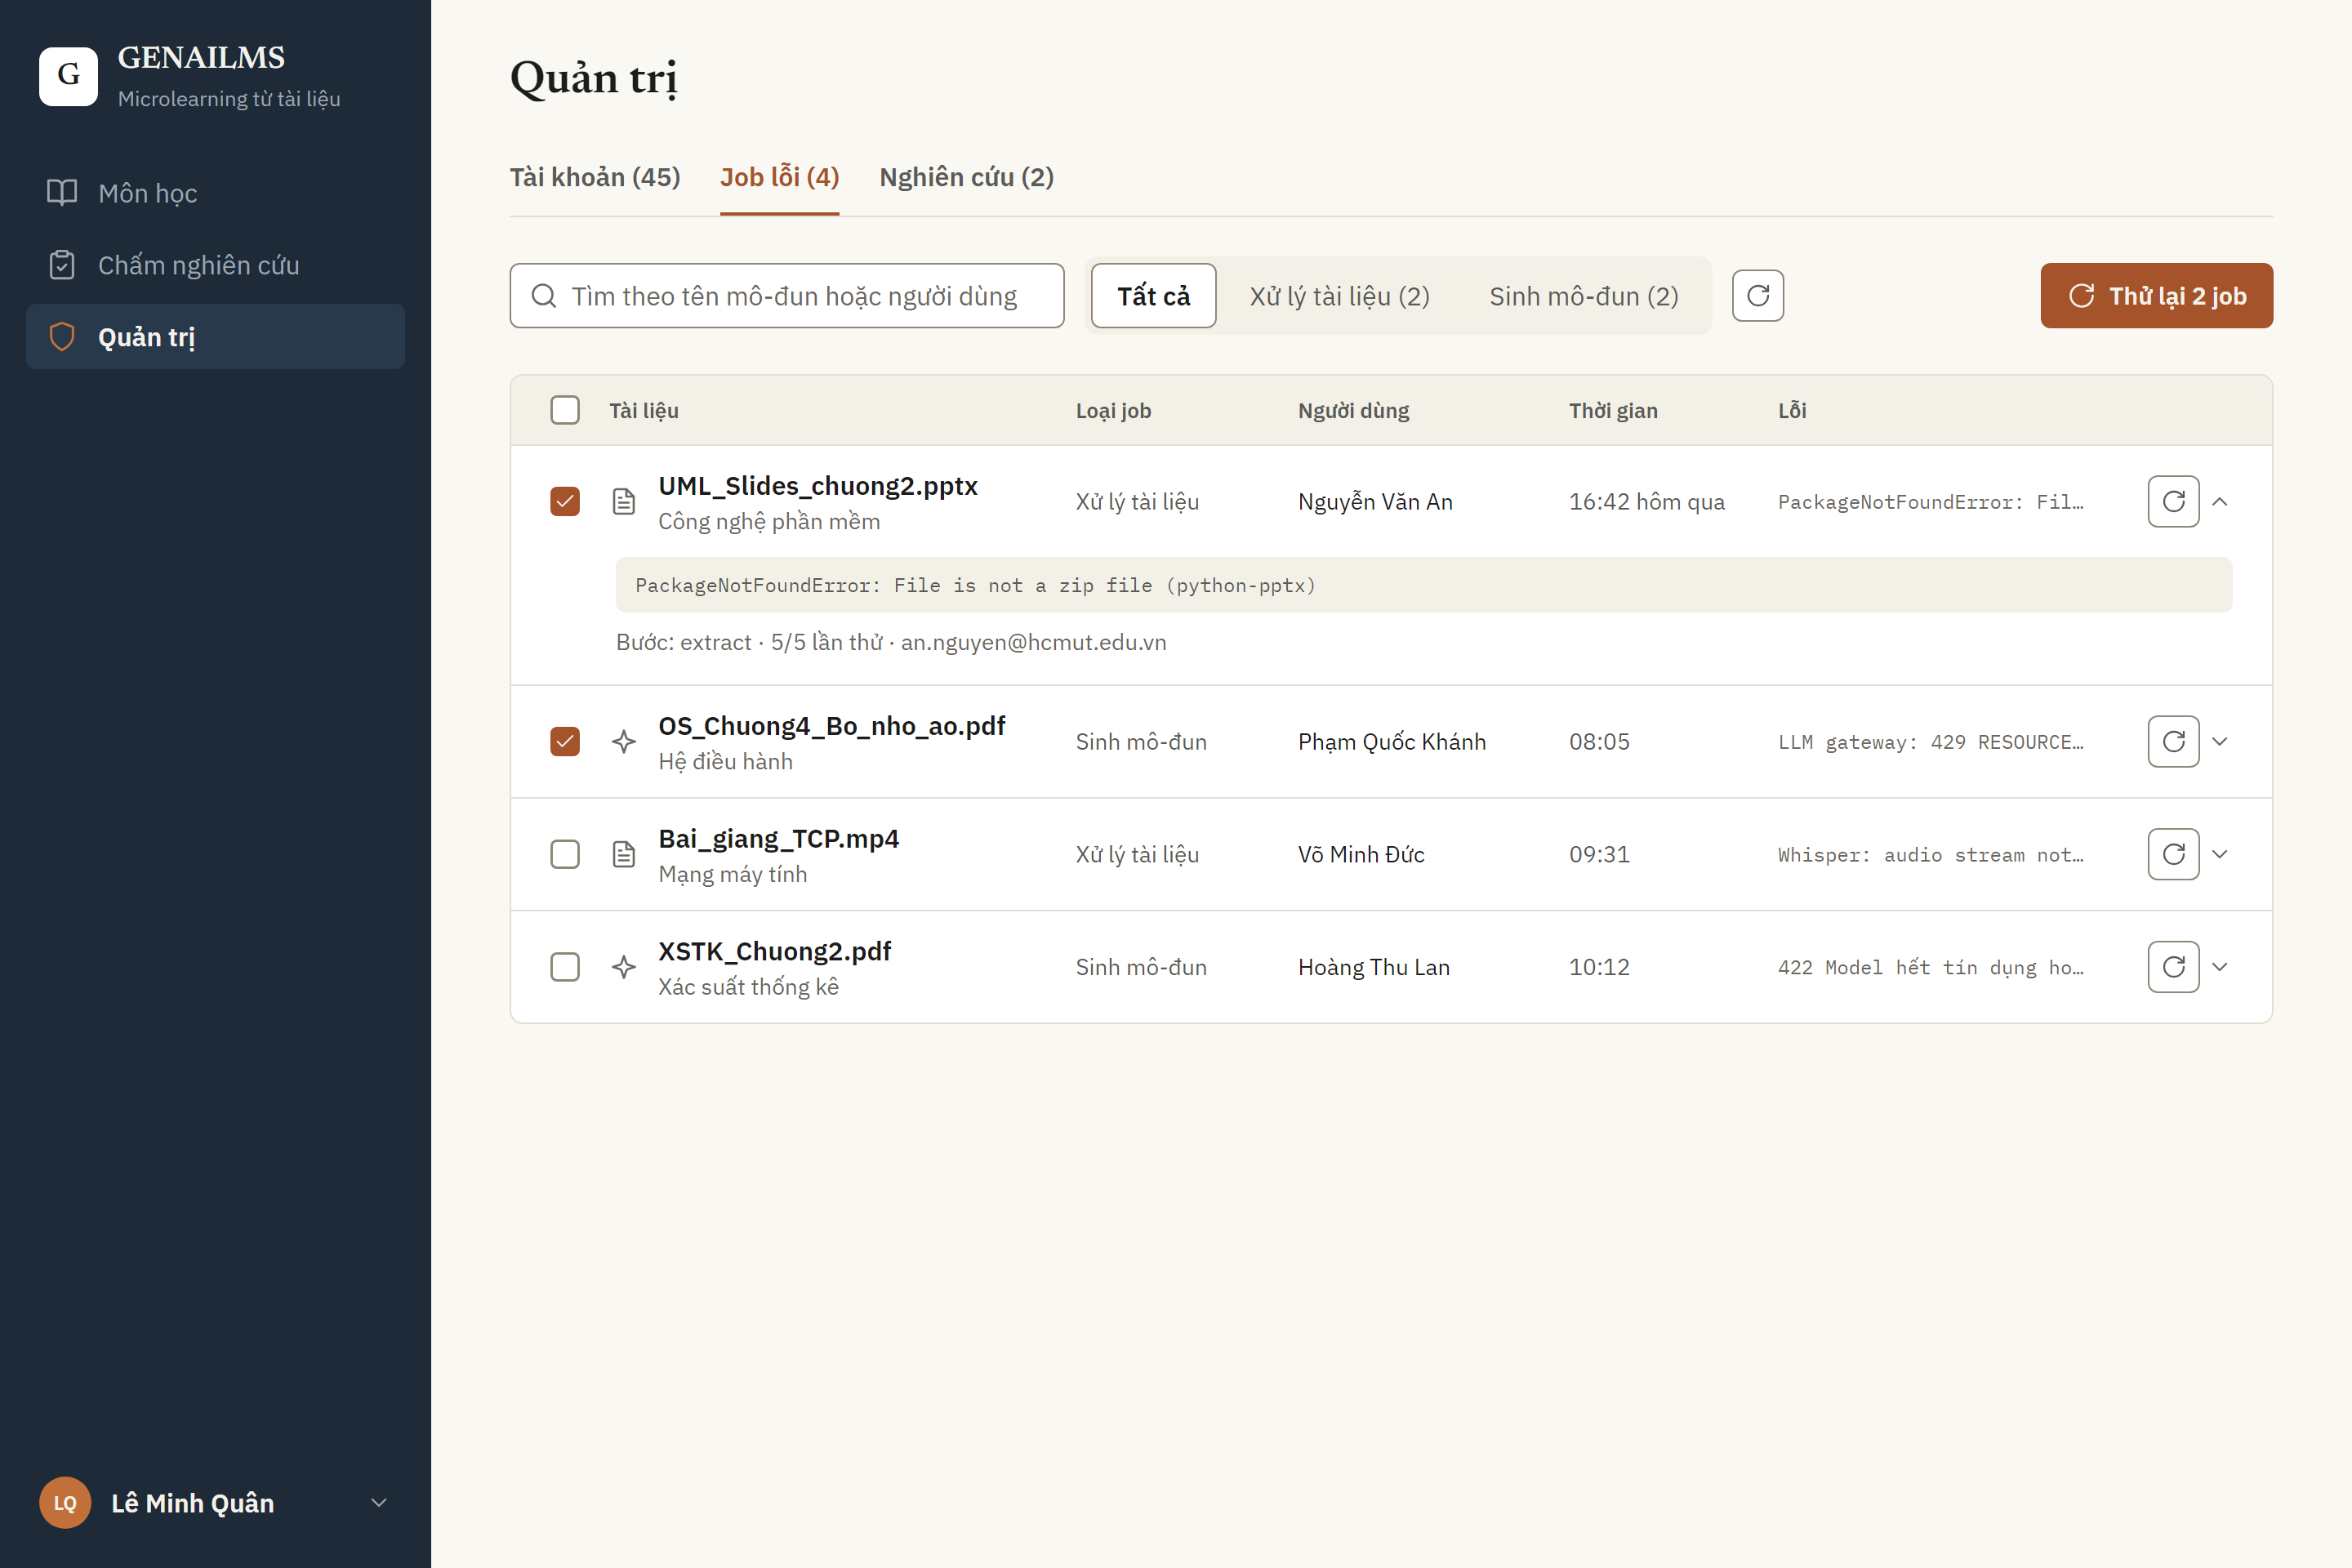
\includegraphics[width=\linewidth,height=.34\textheight,keepaspectratio,viewport={1200 850 2820 1550},clip]{graphics/ui/11-admin-failed-jobs.png}
\caption{Failed-job inspection and recovery.}\label{fig:ui-screen-11}
\end{figure}

\needspace{.42\textheight}
Figure~\ref{fig:ui-screen-12} groups study identity, snapshot preparation and rater invitations in an administrative workspace. ``Nghiên cứu'' means ``Study''; anonymous packet preparation precedes activation for raters.
\begin{figure}[H]\centering
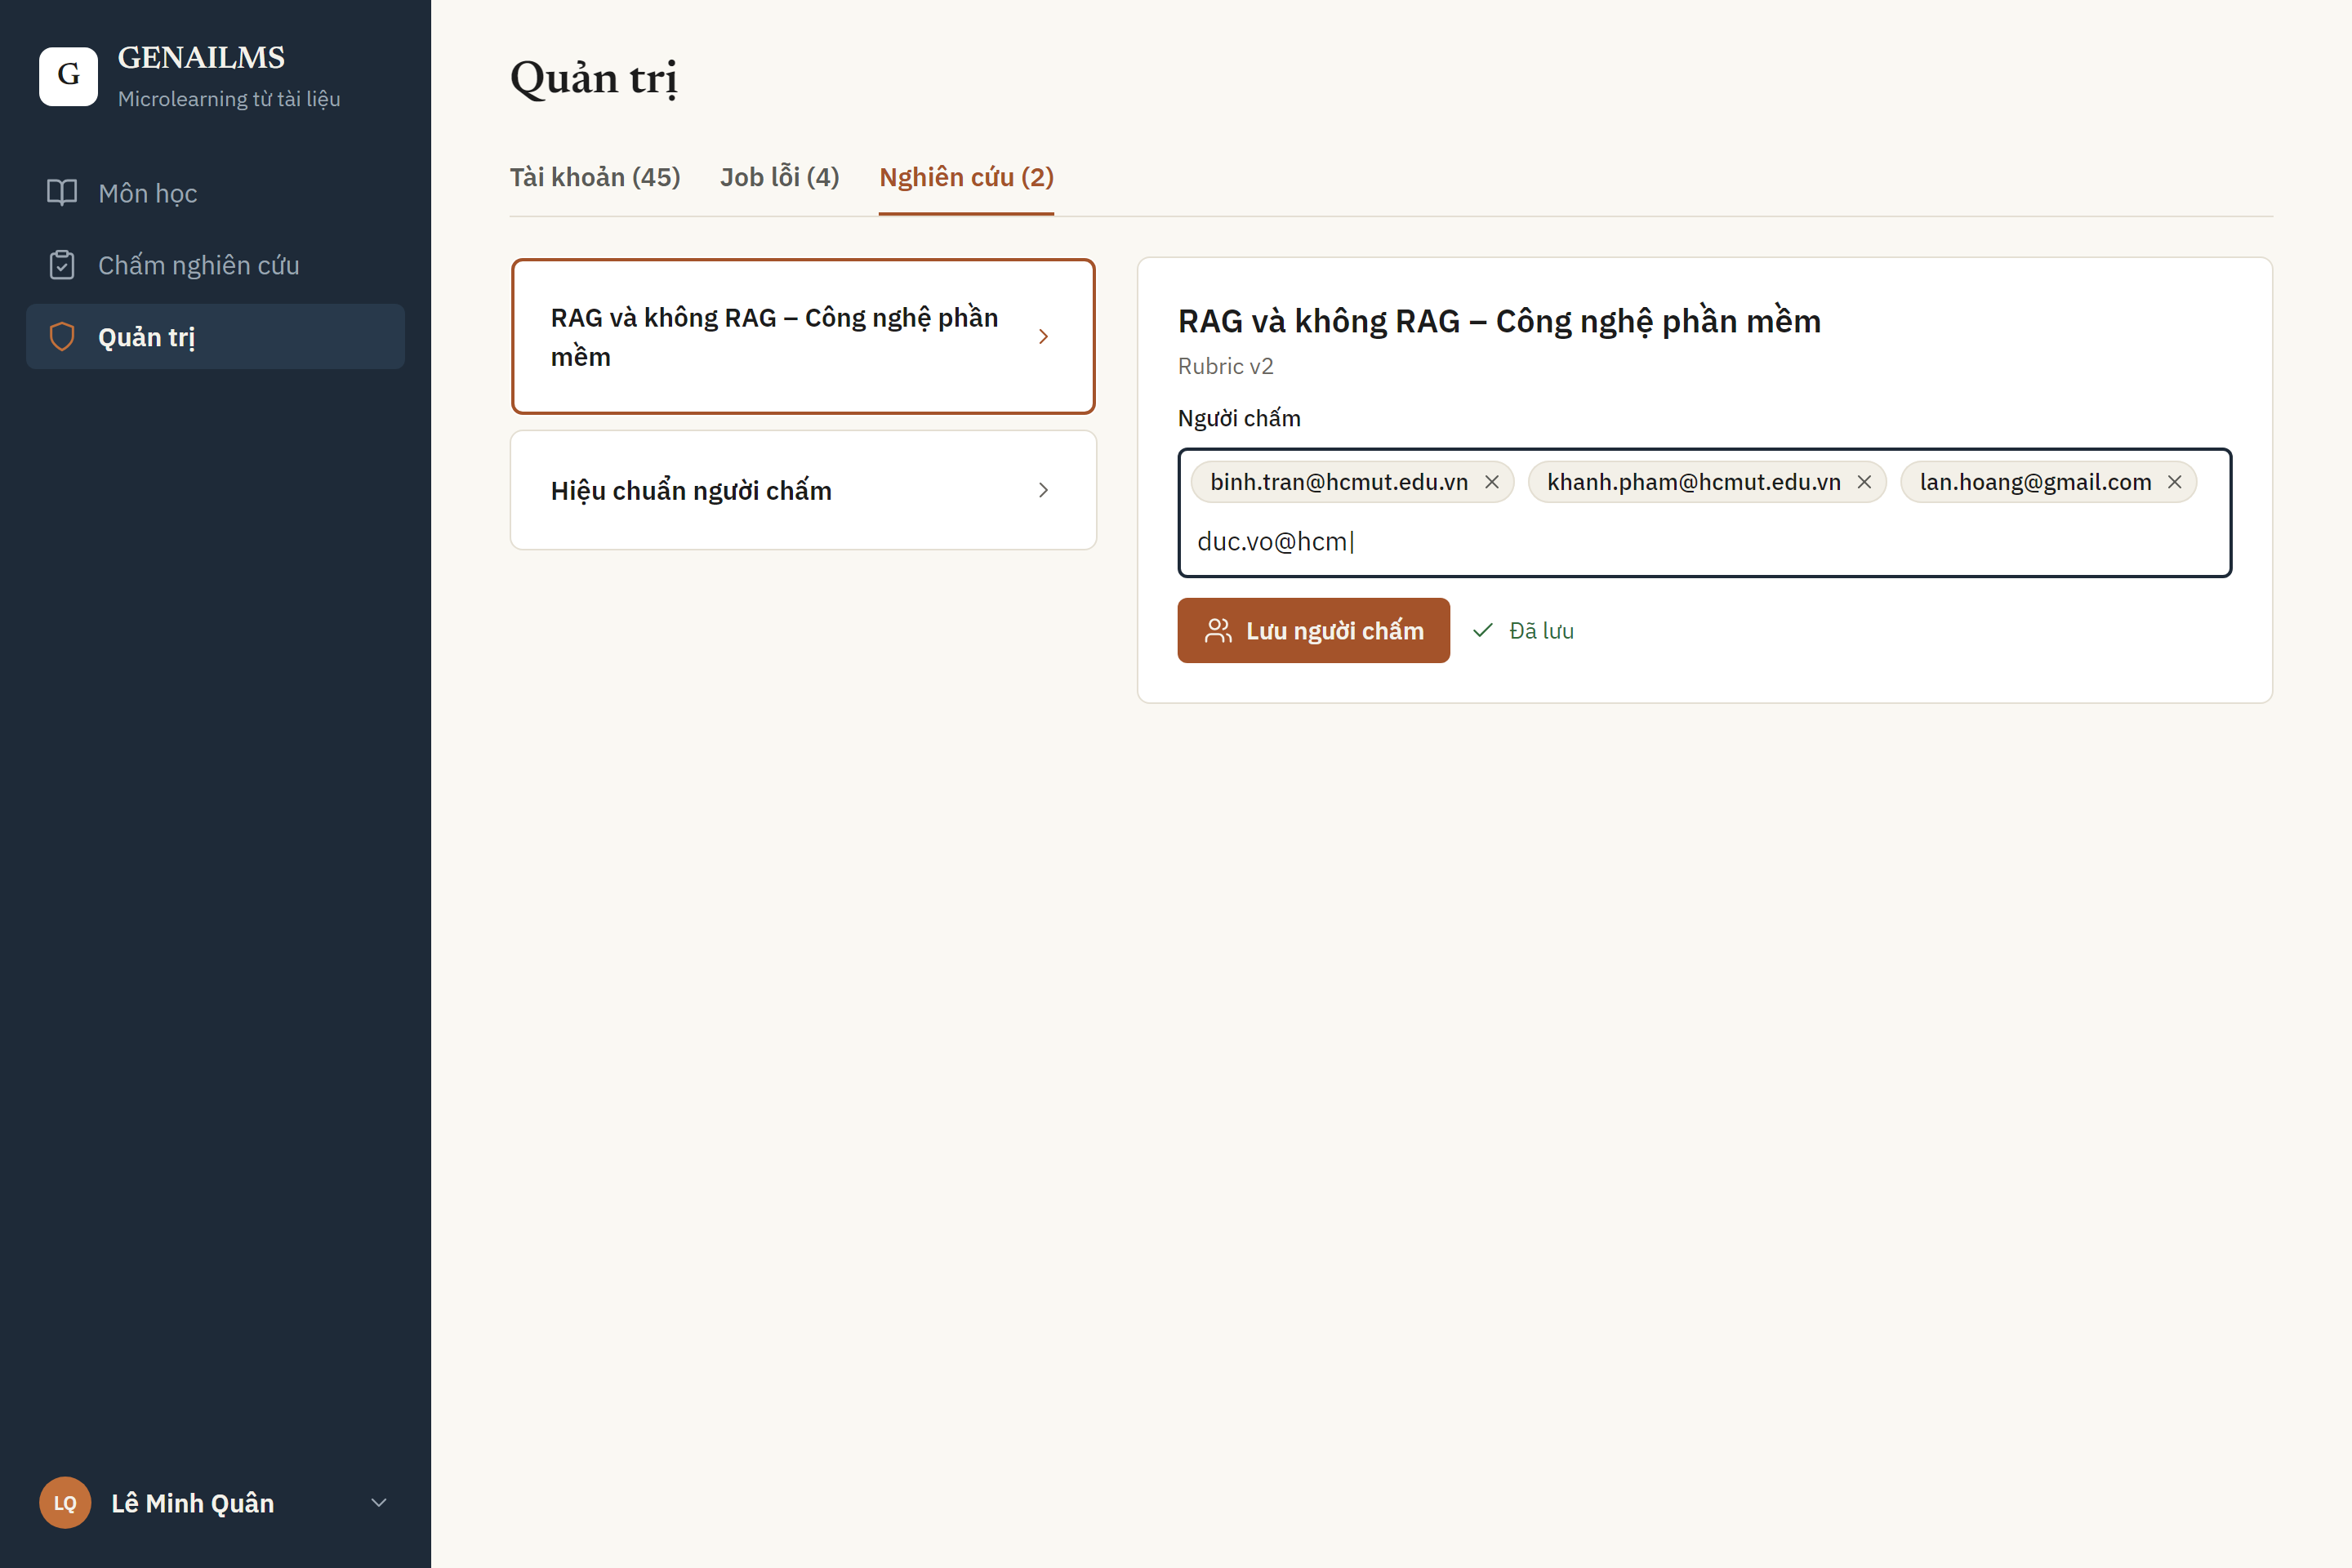
\includegraphics[width=\linewidth,height=.34\textheight,keepaspectratio,viewport={1370 1030 2810 1630},clip]{graphics/ui/12-admin-studies.png}
\caption{Study preparation and invitations.}\label{fig:ui-screen-12}
\end{figure}

\needspace{.42\textheight}
Figure~\ref{fig:ui-screen-13} enlarges the scoring controls and the reason field in the blinded-rating screen. ``Nhận xét'' means ``Comment''; the 1--5 controls and written reasons are recorded per criterion while the packet order remains stable for the rater.
\begin{figure}[H]\centering
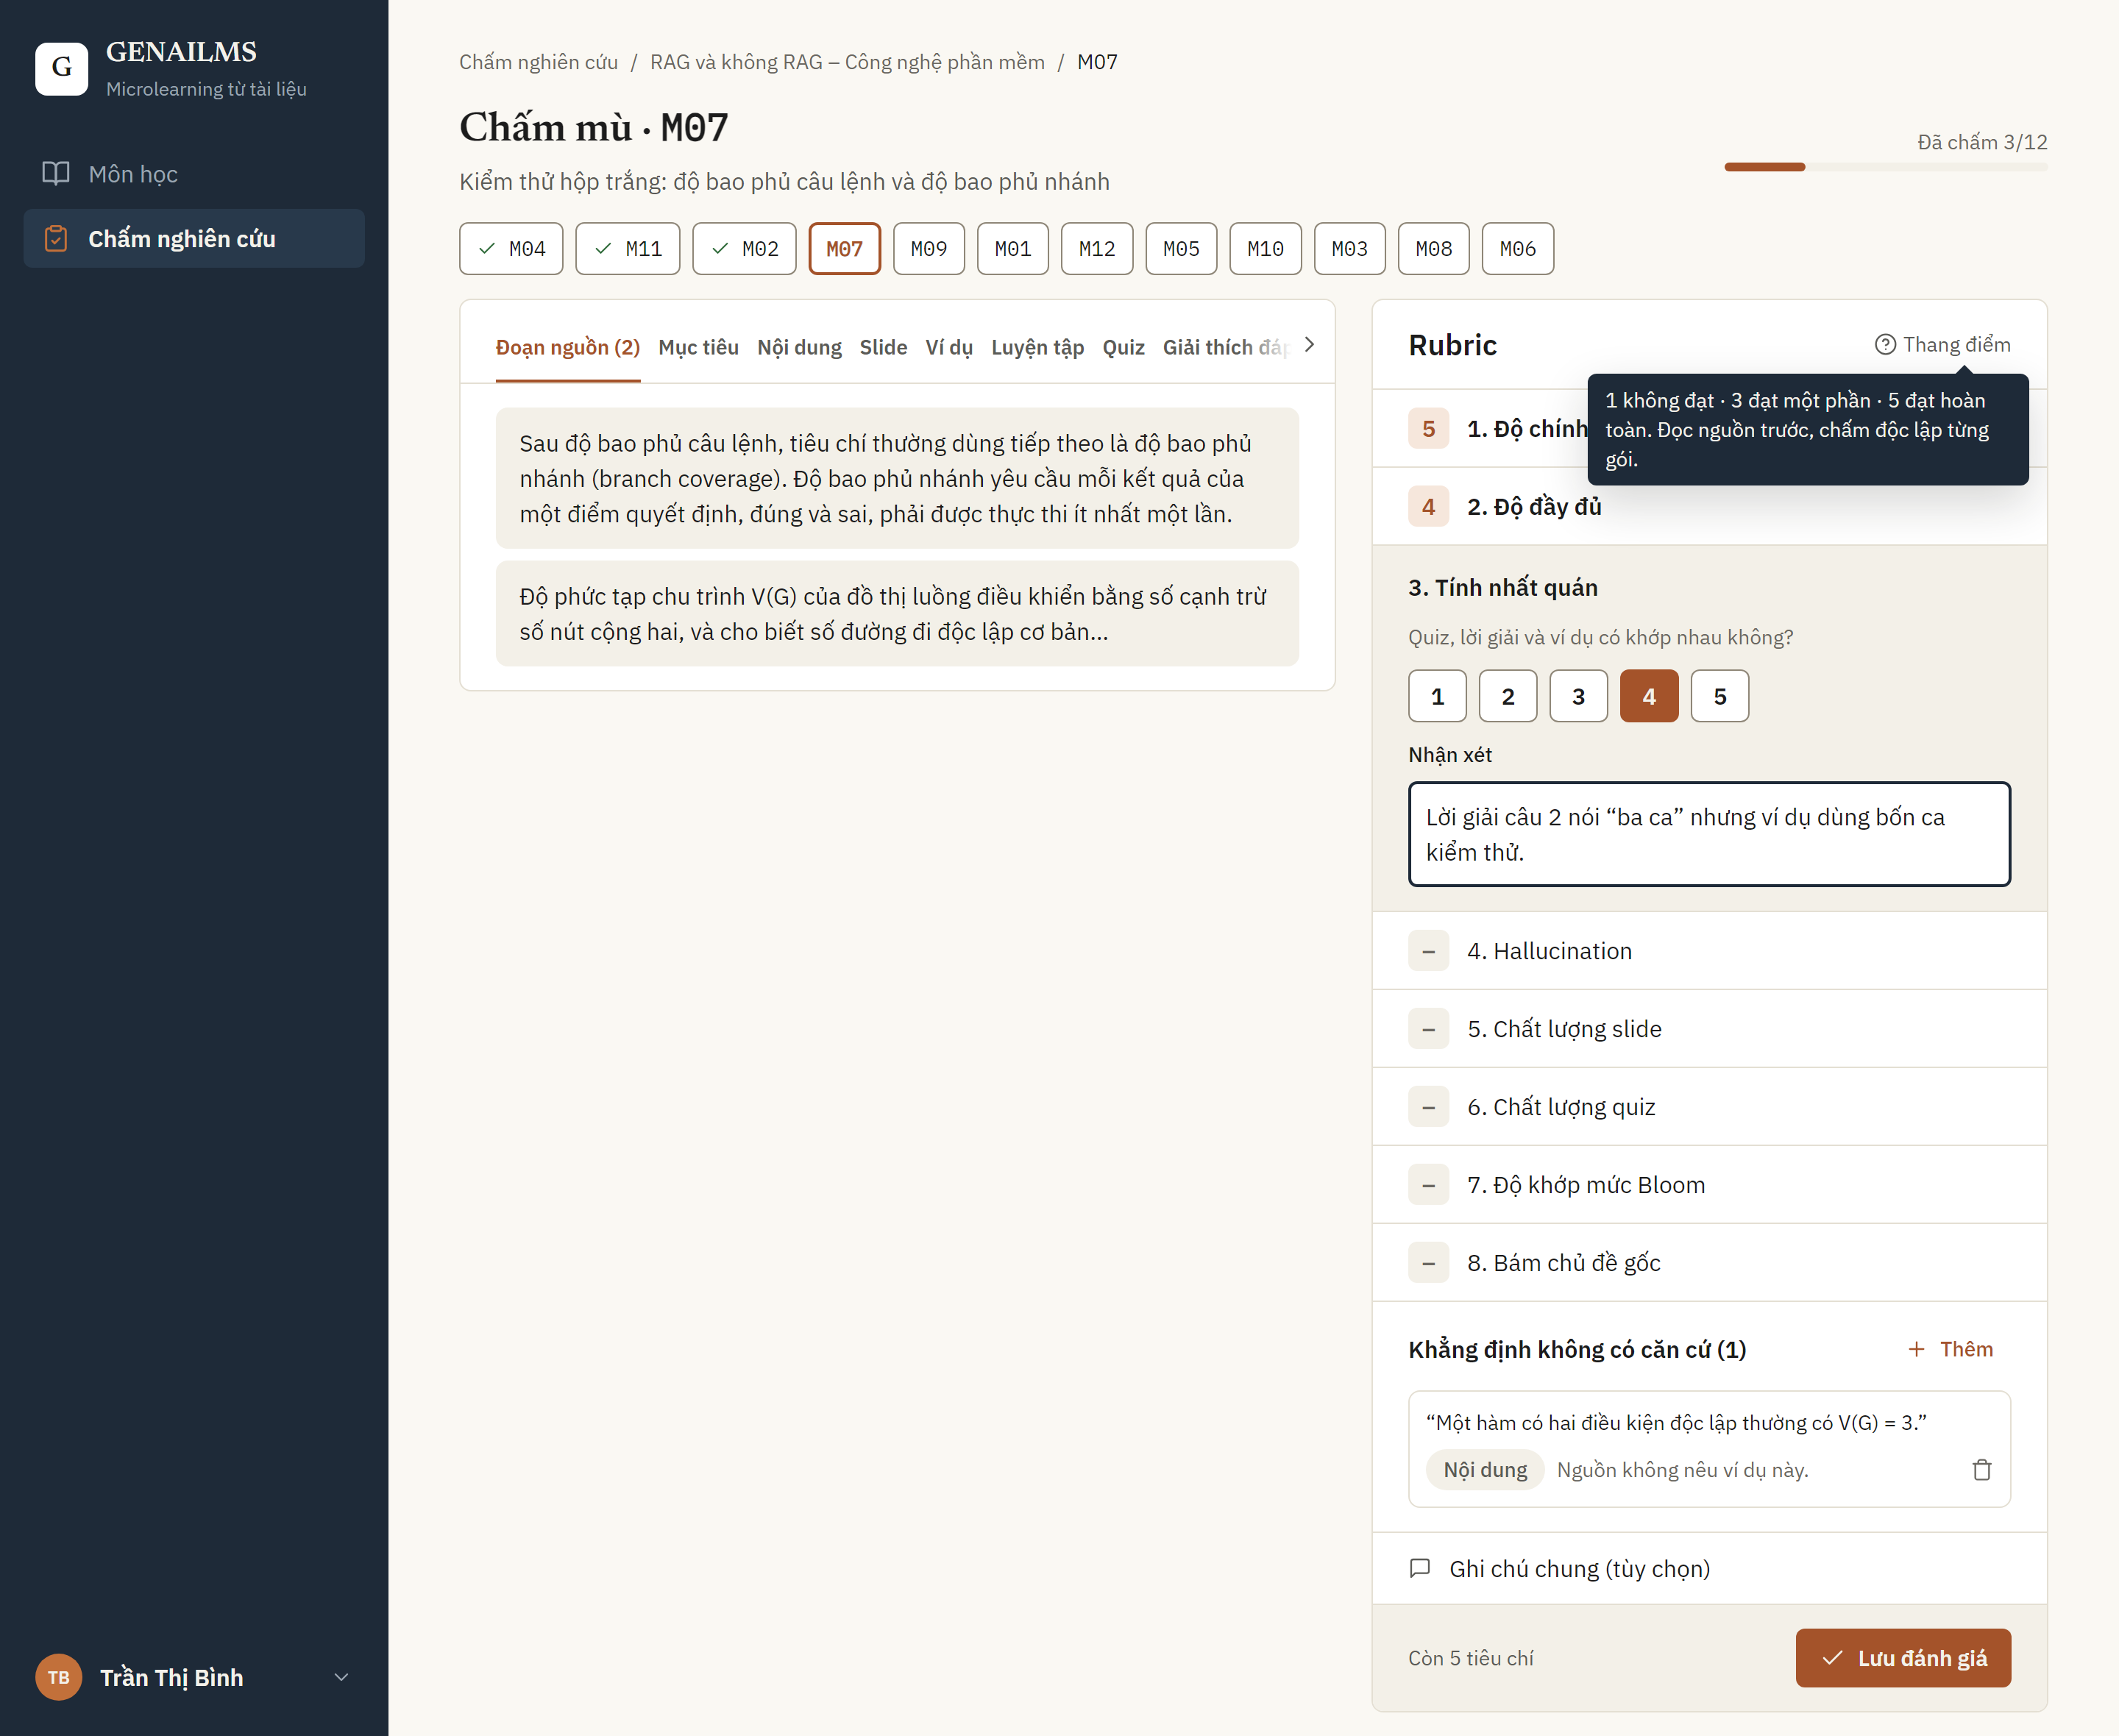
\includegraphics[width=\linewidth,height=.34\textheight,keepaspectratio,viewport={1850 1100 2800 1580},clip]{graphics/ui/13-rater-blind-rating.png}
\caption{Focused rubric and criterion-level reasoning.}\label{fig:ui-screen-13}
\end{figure}

\needspace{.42\textheight}
Figure~\ref{fig:ui-screen-14} shows the course workspace as a single column on a mobile viewport. Upload, status and generation actions retain text labels; secondary information collapses without hiding failure recovery.
\begin{figure}[H]\centering
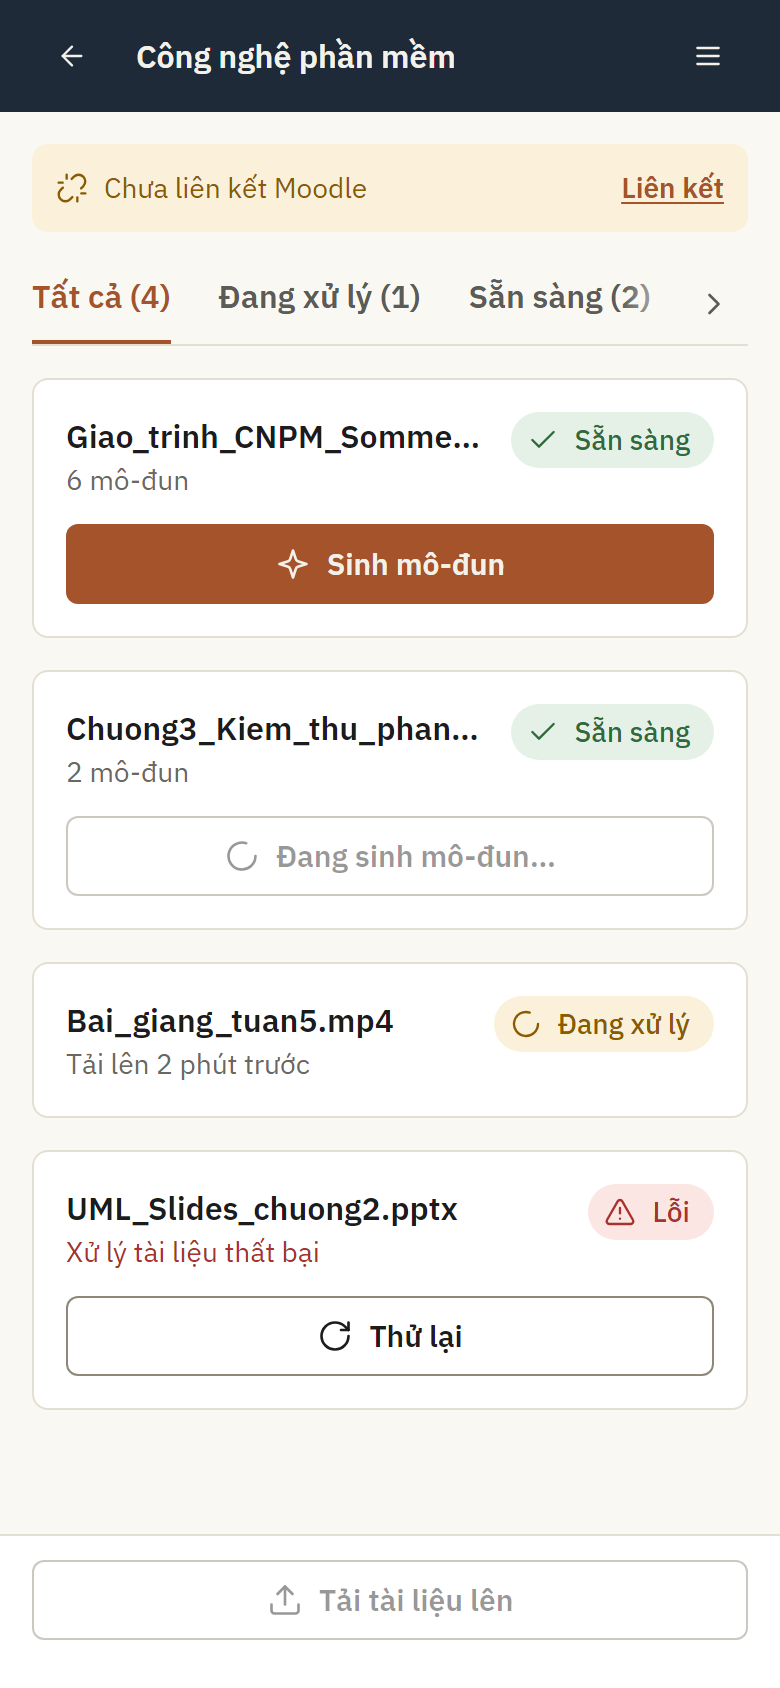
\includegraphics[width=.65\linewidth,height=.60\textheight,keepaspectratio]{graphics/ui/14-mobile-course-detail.png}
\caption{Mobile authoring workspace.}\label{fig:ui-screen-14}
\end{figure}

\needspace{.42\textheight}
Figure~\ref{fig:ui-screen-15} shows empty-course, empty-document and loading panels. ``Chưa có môn học'' means ``No courses yet'' and ``Chọn tệp'' means ``Choose file''; useful next actions appear directly in the empty state.
\begin{figure}[H]\centering
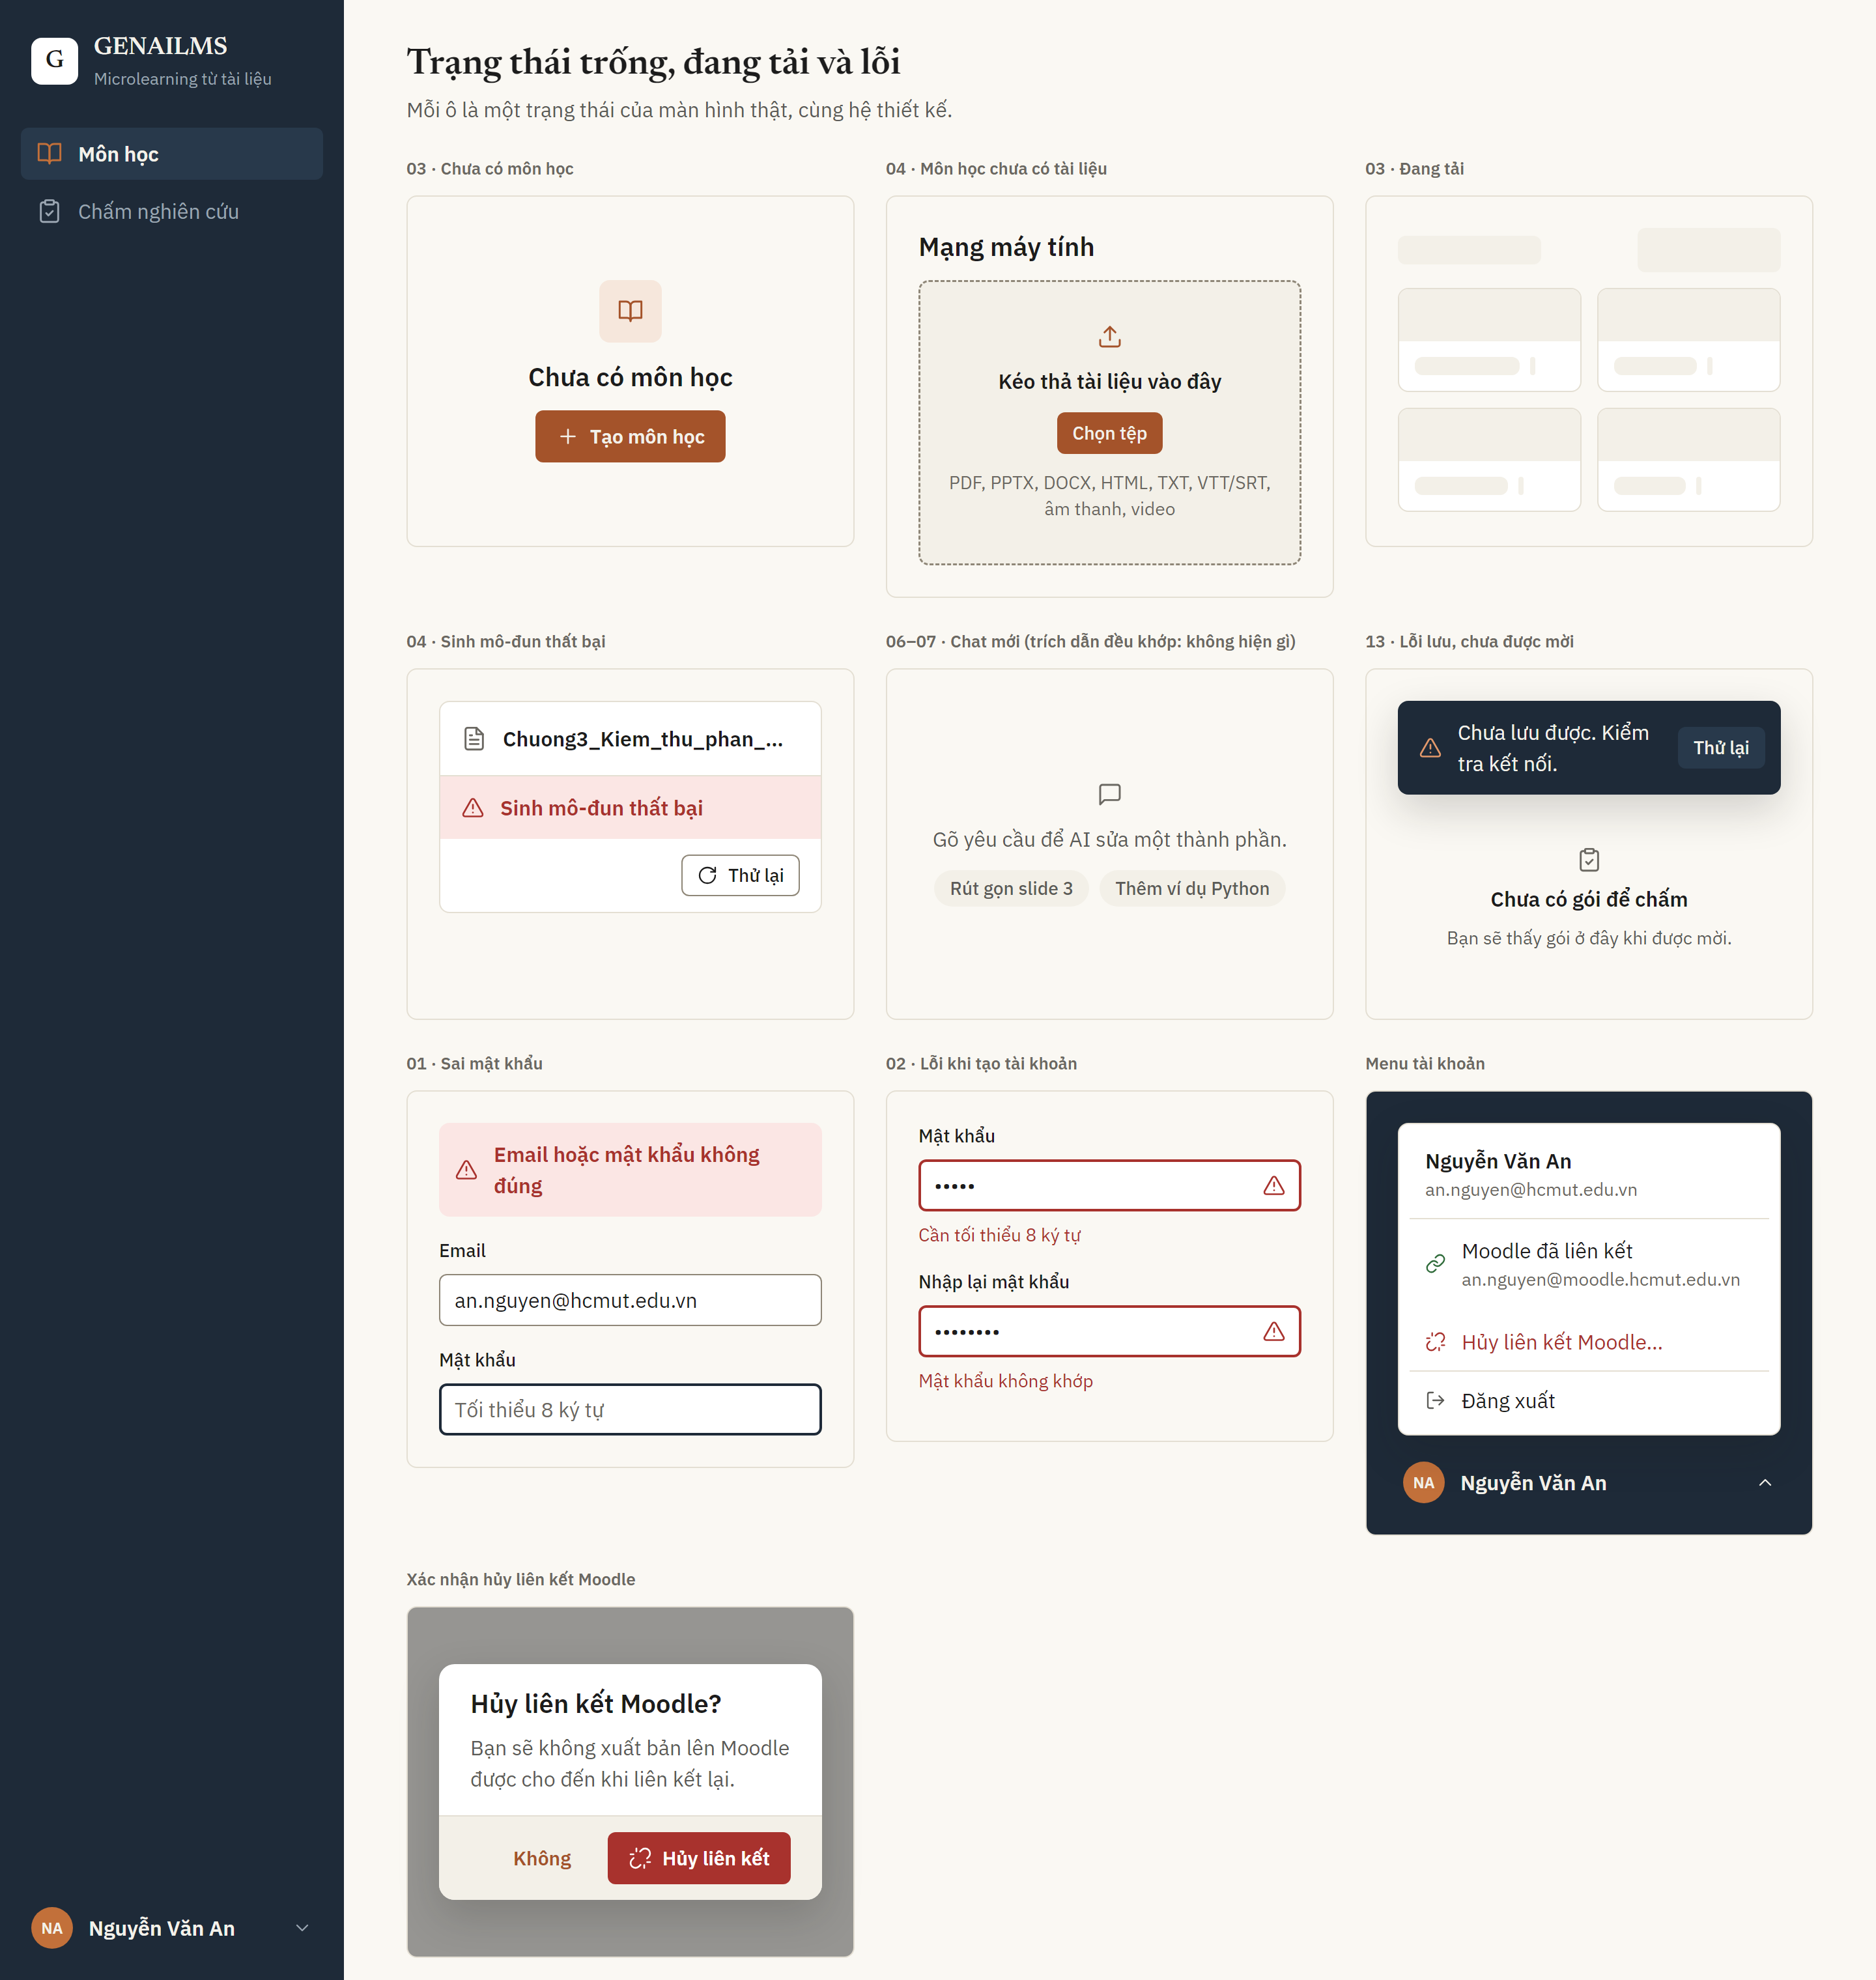
\includegraphics[width=.47\linewidth,height=.26\textheight,keepaspectratio,viewport={620 2200 1320 2750},clip]{graphics/ui/15-empty-loading-error-states.png}\hfill
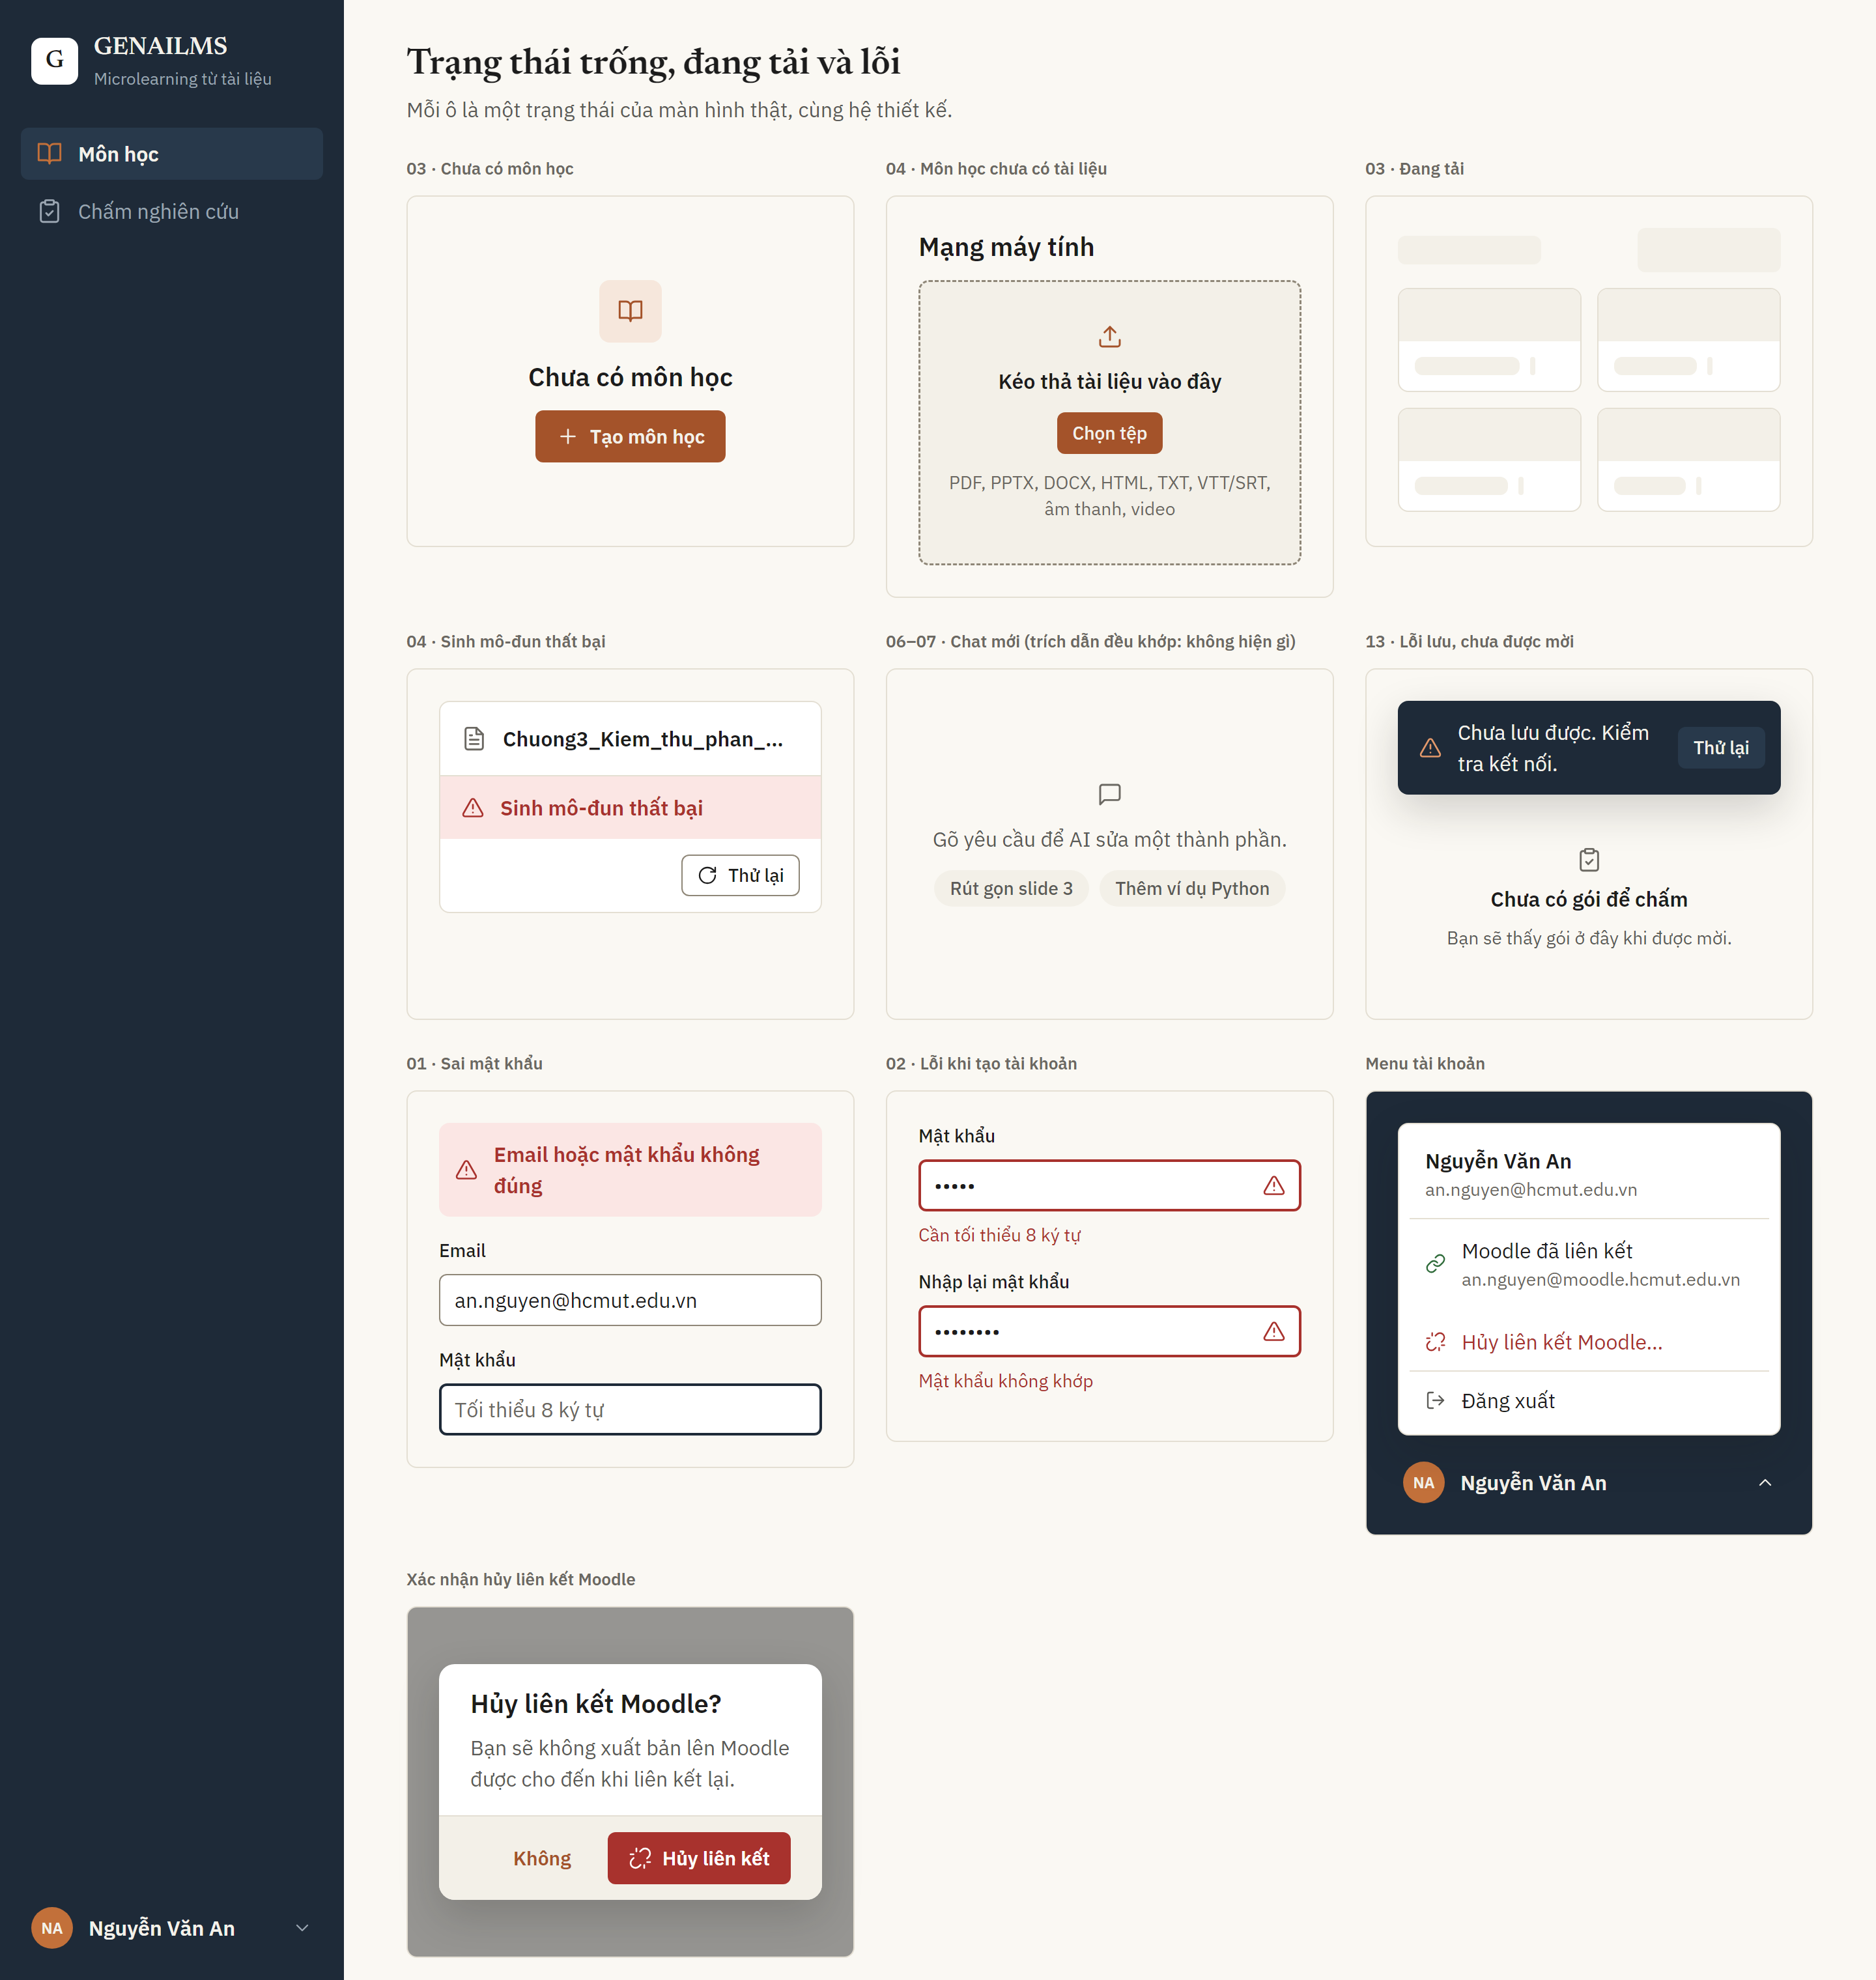
\includegraphics[width=.47\linewidth,height=.26\textheight,keepaspectratio,viewport={1360 2110 2050 2750},clip]{graphics/ui/15-empty-loading-error-states.png}\par\smallskip
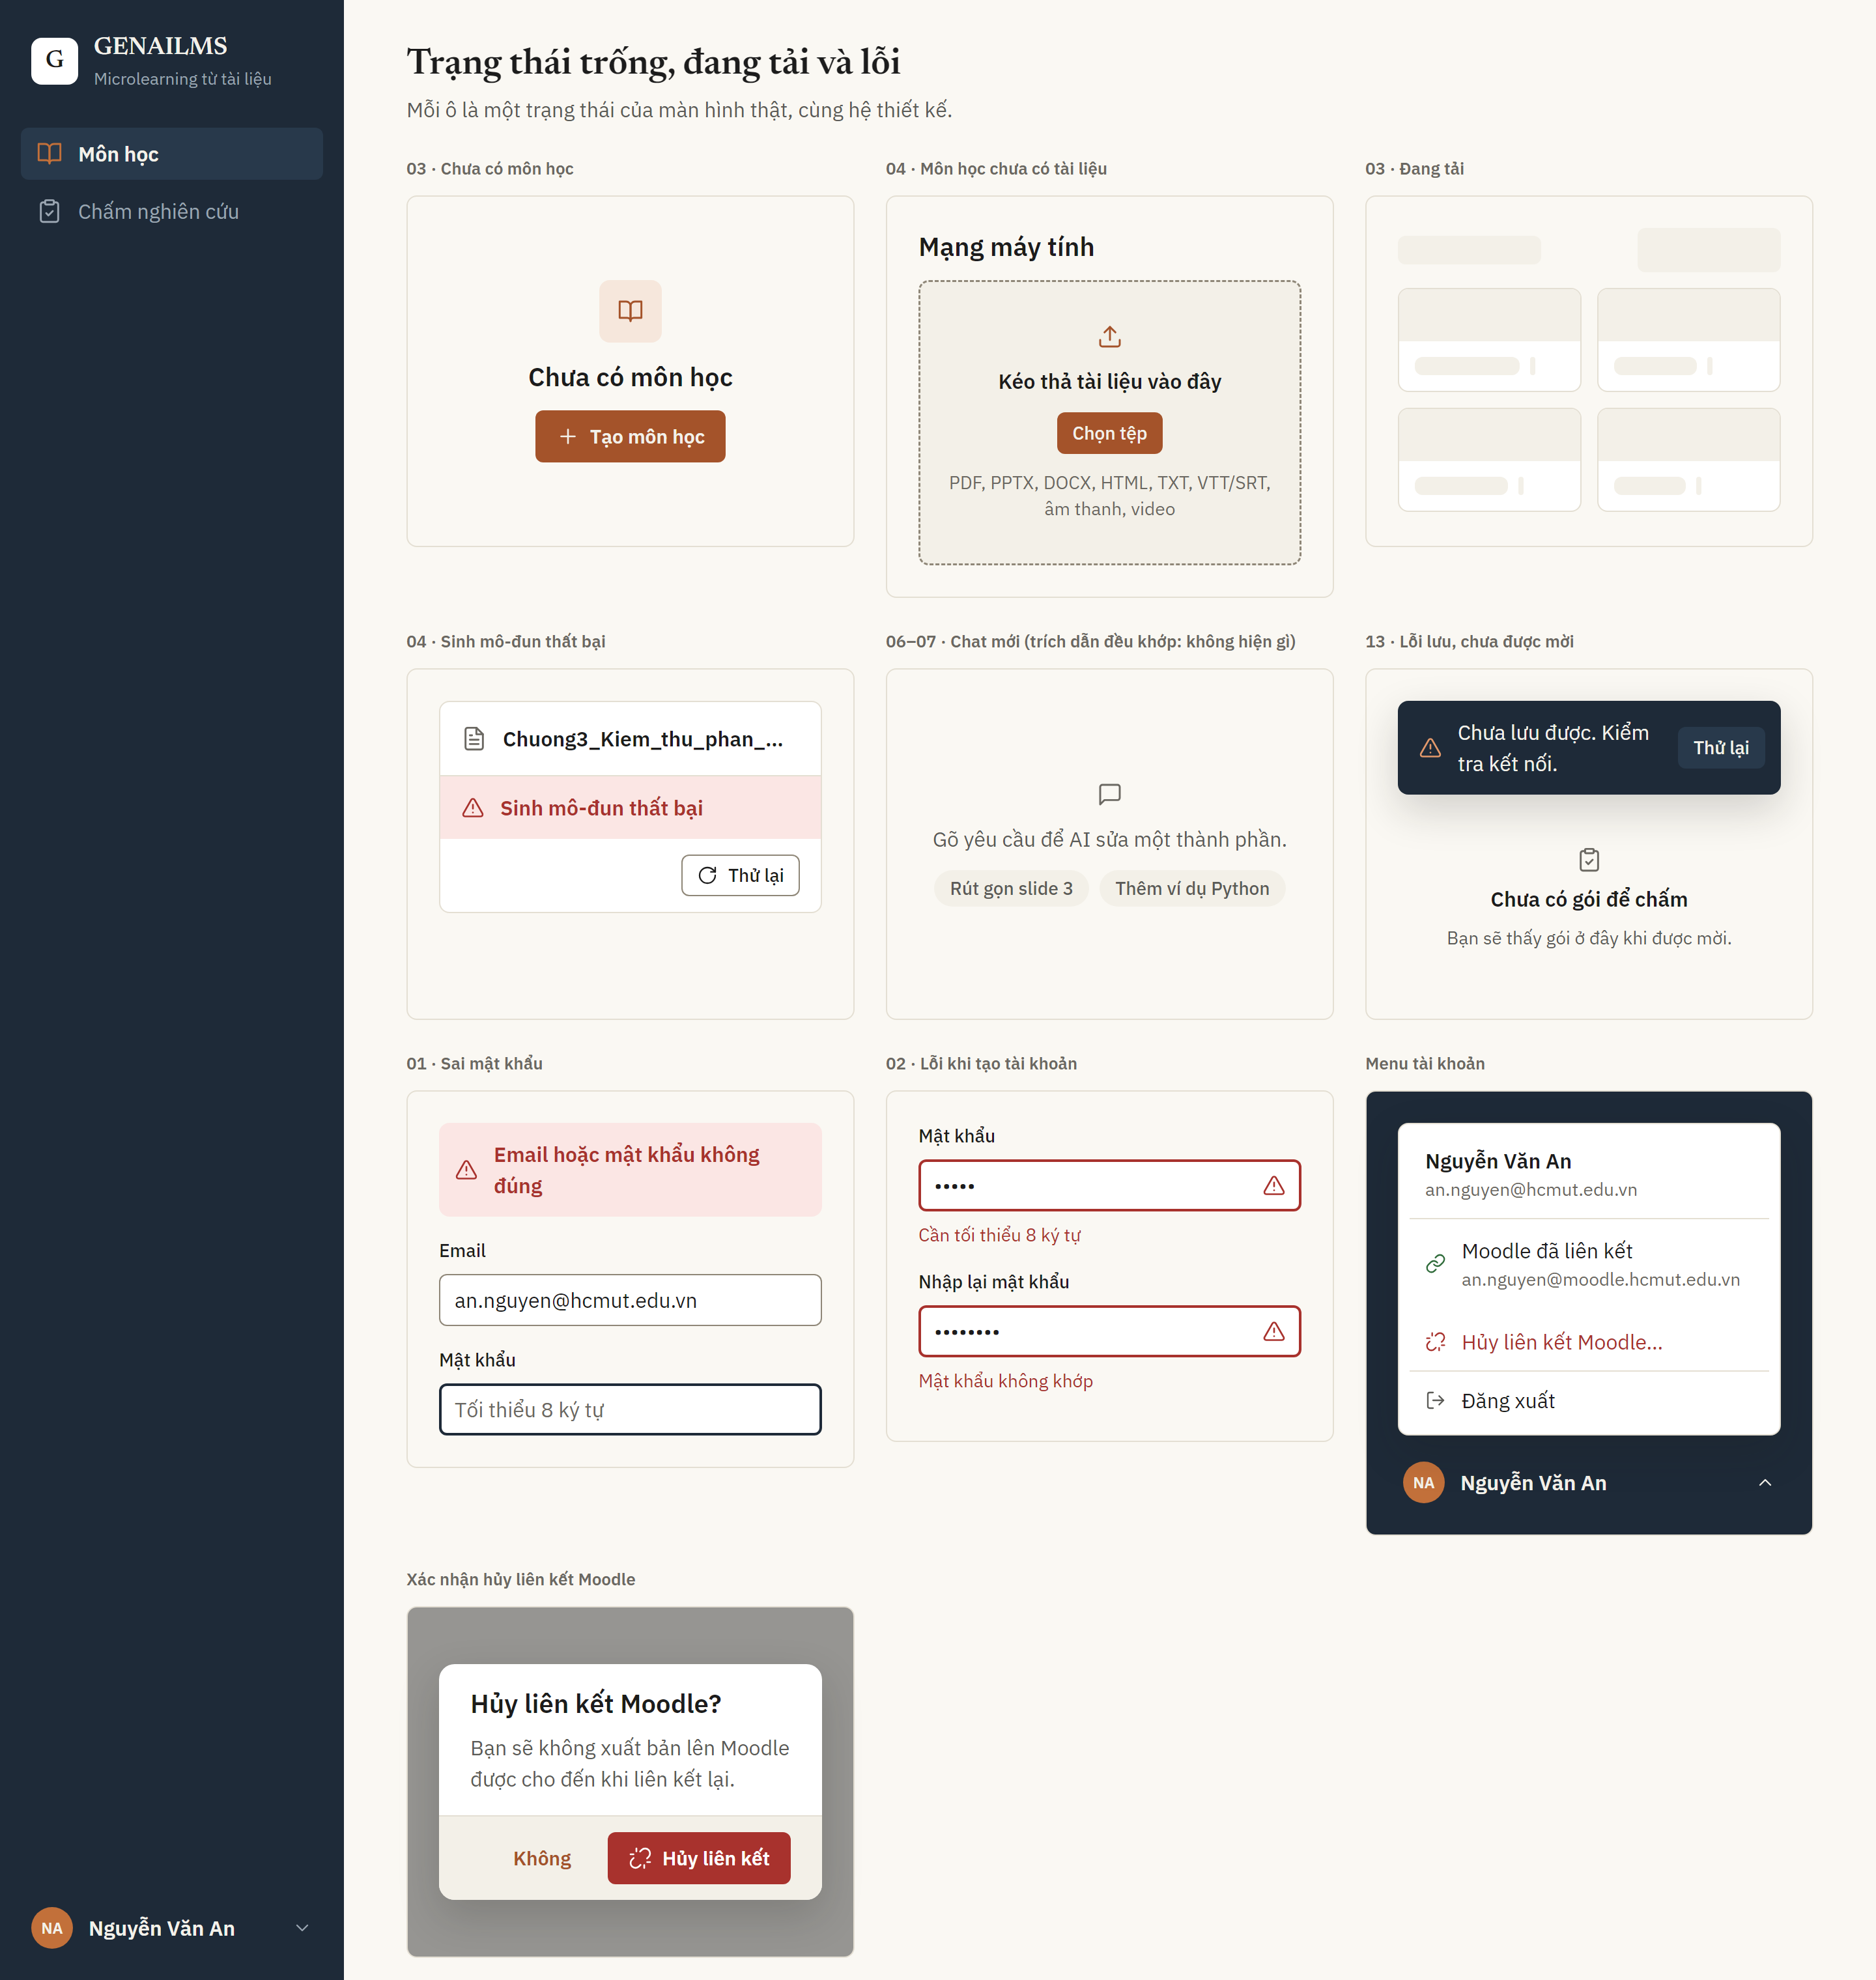
\includegraphics[width=.47\linewidth,height=.26\textheight,keepaspectratio,viewport={2100 2200 2800 2750},clip]{graphics/ui/15-empty-loading-error-states.png}\hfill
\caption{Empty and loading states.}\label{fig:ui-screen-15}
\end{figure}

\needspace{.42\textheight}
Figure~\ref{fig:ui-screen-15-recovery} groups generation failure, an empty editing conversation and a failed rating save. ``Chưa lưu được'' means ``Could not save''; the interface preserves entered work and offers retry.
\begin{figure}[H]\centering
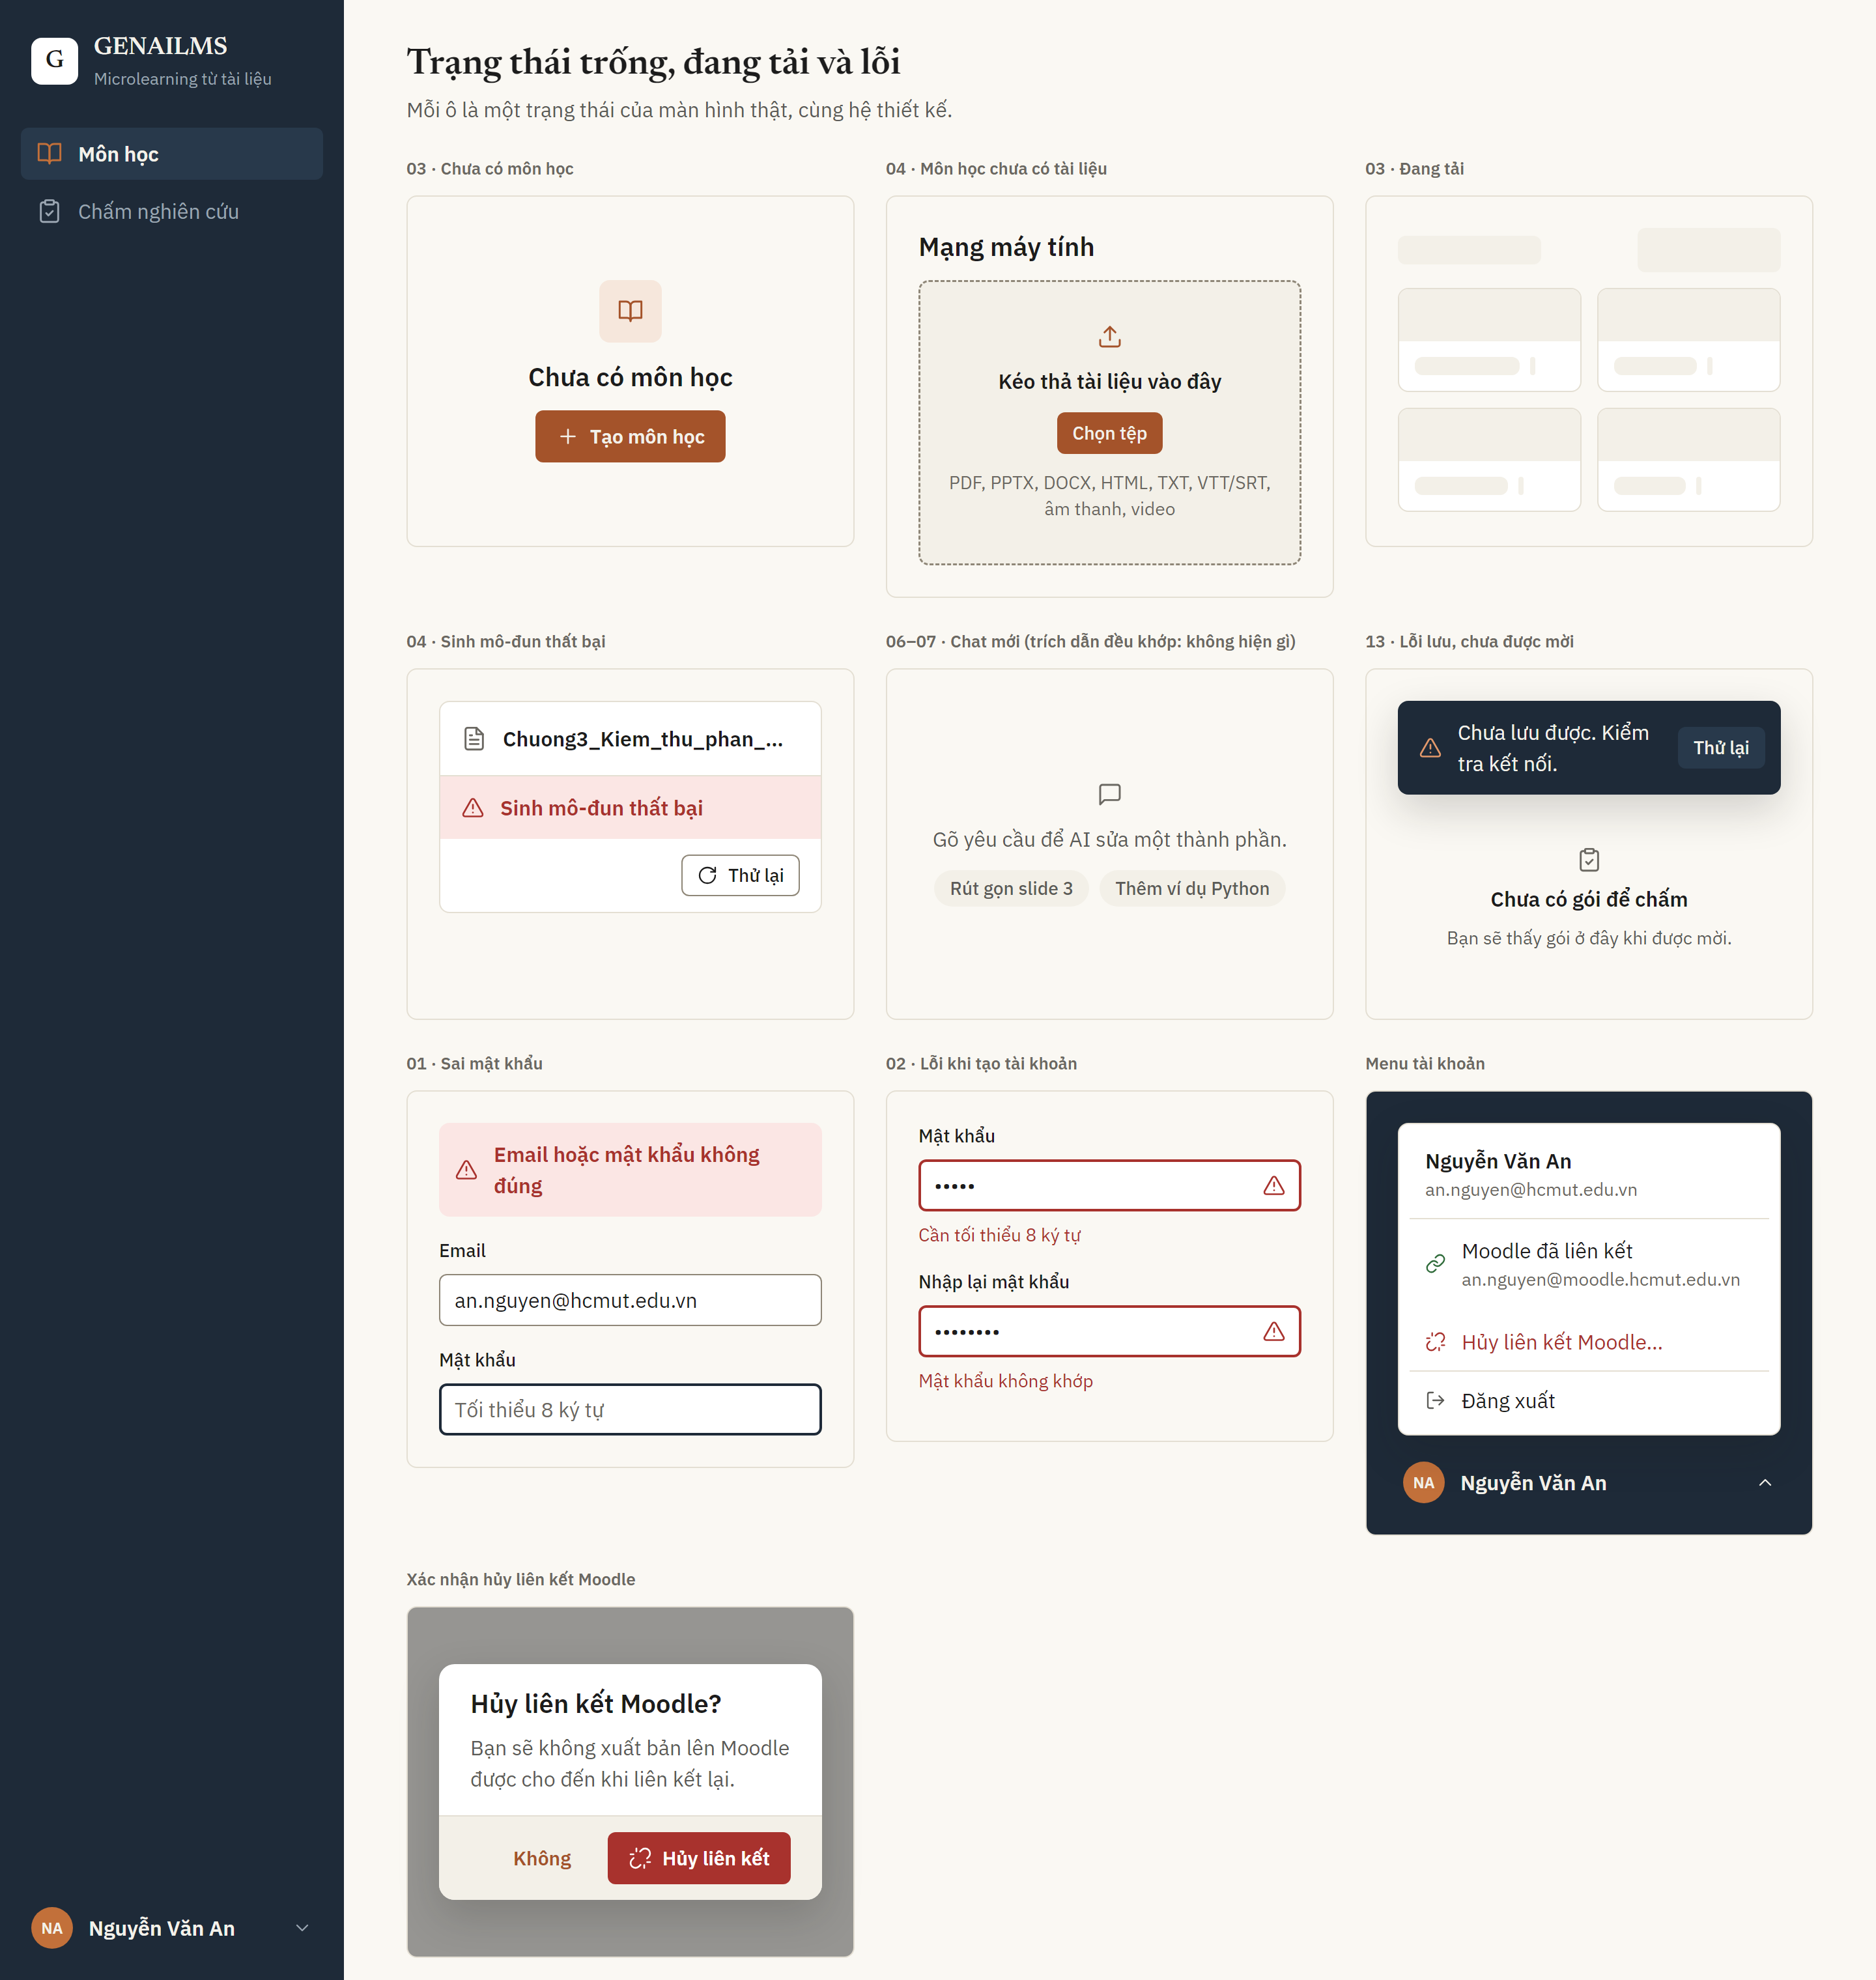
\includegraphics[width=.47\linewidth,height=.26\textheight,keepaspectratio,viewport={620 1480 1320 2000},clip]{graphics/ui/15-empty-loading-error-states.png}\hfill
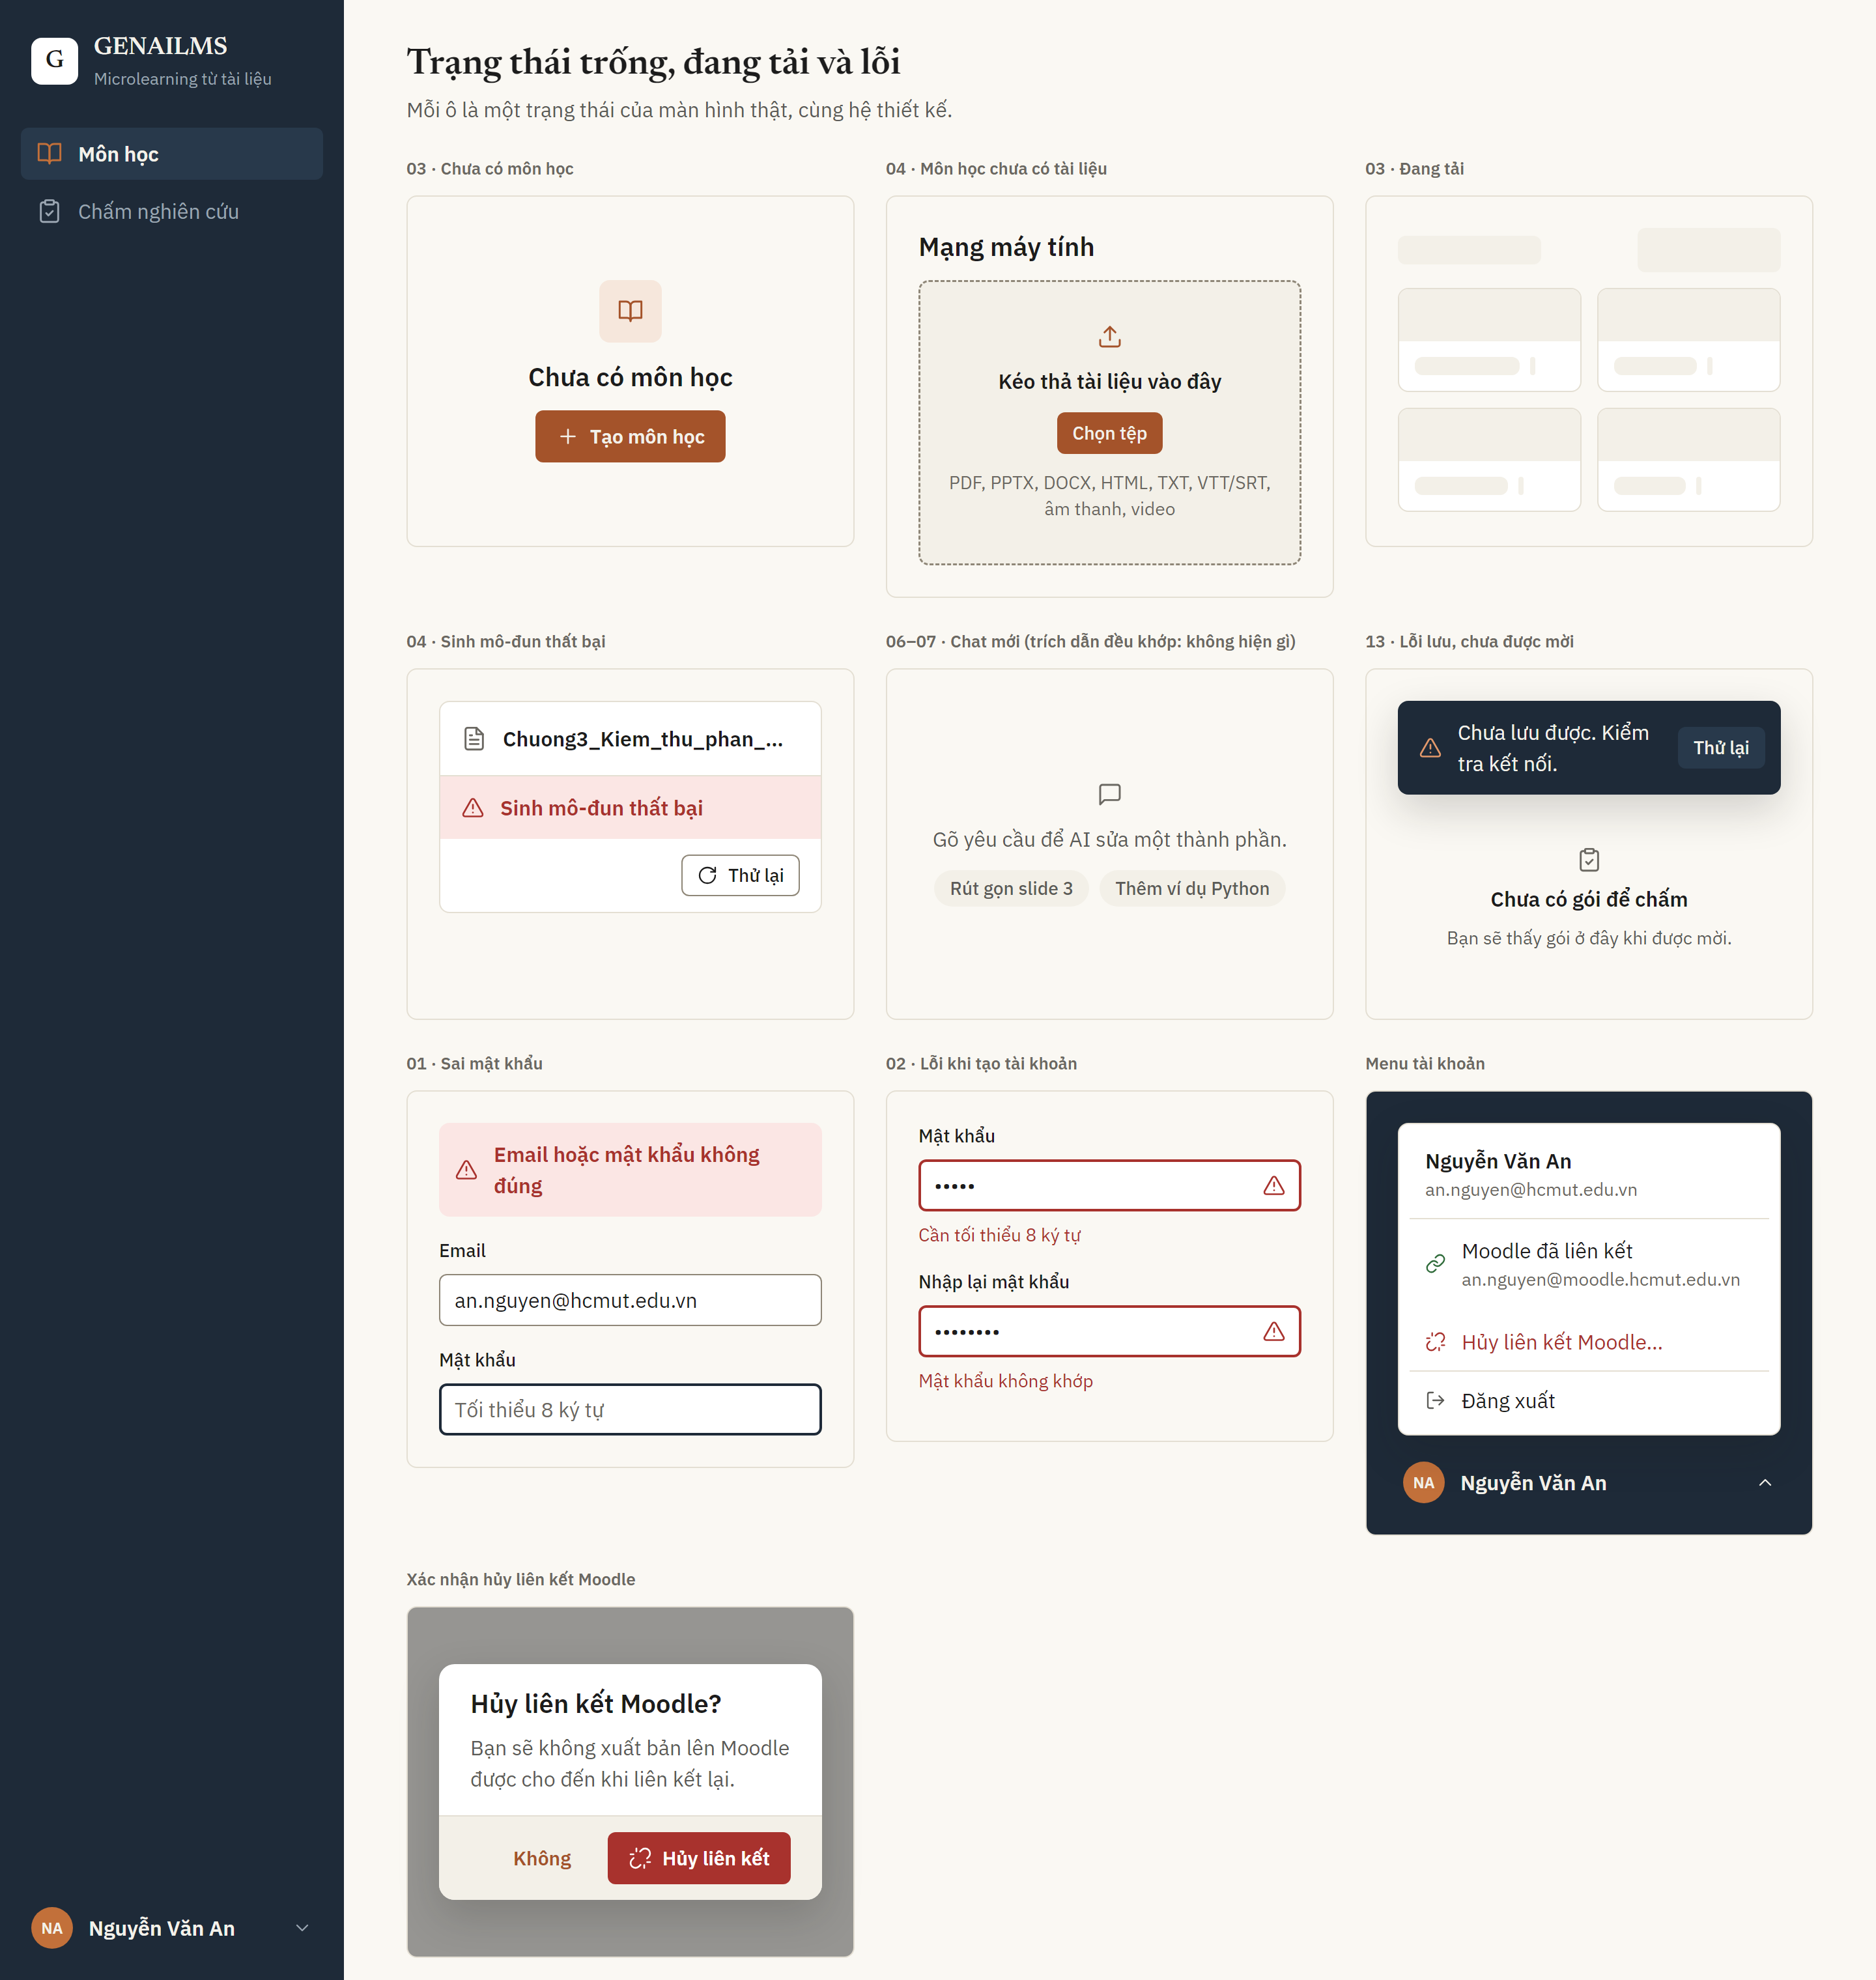
\includegraphics[width=.47\linewidth,height=.26\textheight,keepaspectratio,viewport={1360 1480 2050 2000},clip]{graphics/ui/15-empty-loading-error-states.png}\par\smallskip
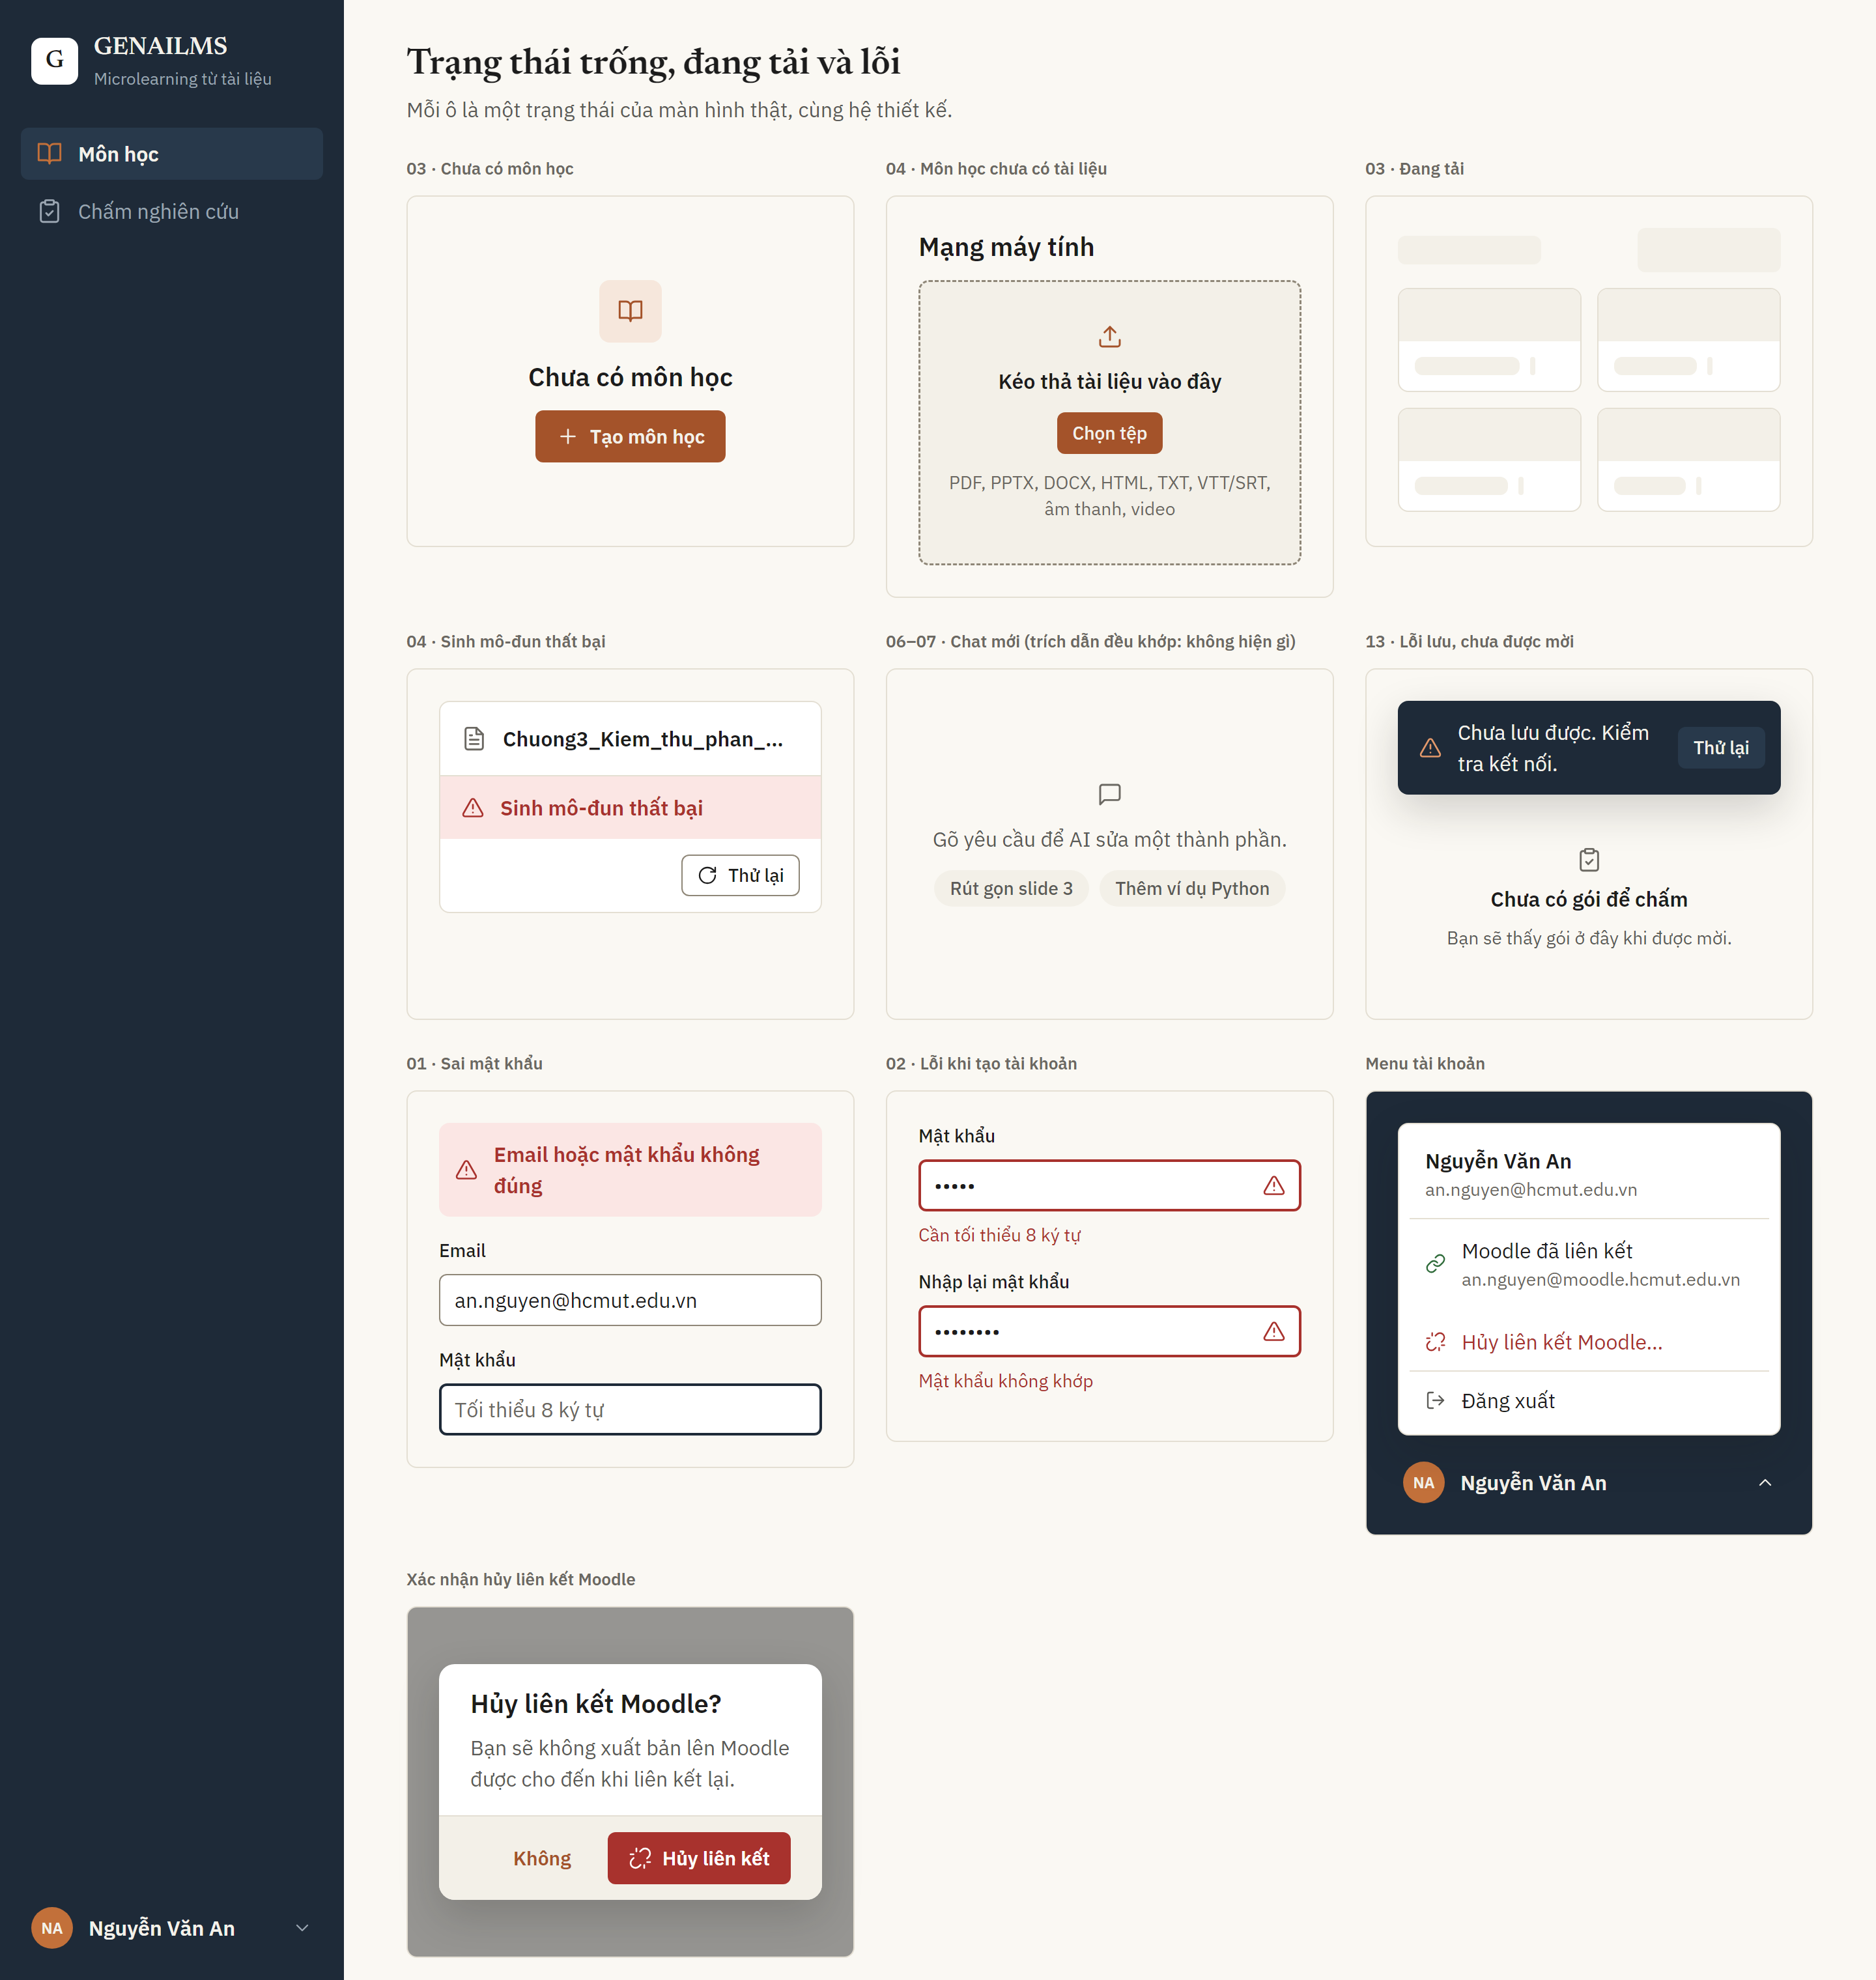
\includegraphics[width=.47\linewidth,height=.26\textheight,keepaspectratio,viewport={2100 1480 2800 2000},clip]{graphics/ui/15-empty-loading-error-states.png}\hfill
\caption{Failure recovery and empty conversation.}\label{fig:ui-screen-15-recovery}
\end{figure}

\needspace{.42\textheight}
Figure~\ref{fig:ui-screen-15-account} enlarges credential validation and account controls. ``Hủy liên kết Moodle'' means ``Unlink Moodle'' and ``Đăng xuất'' means ``Sign out''; unlinking requires confirmation because publication access changes.
\begin{figure}[H]\centering
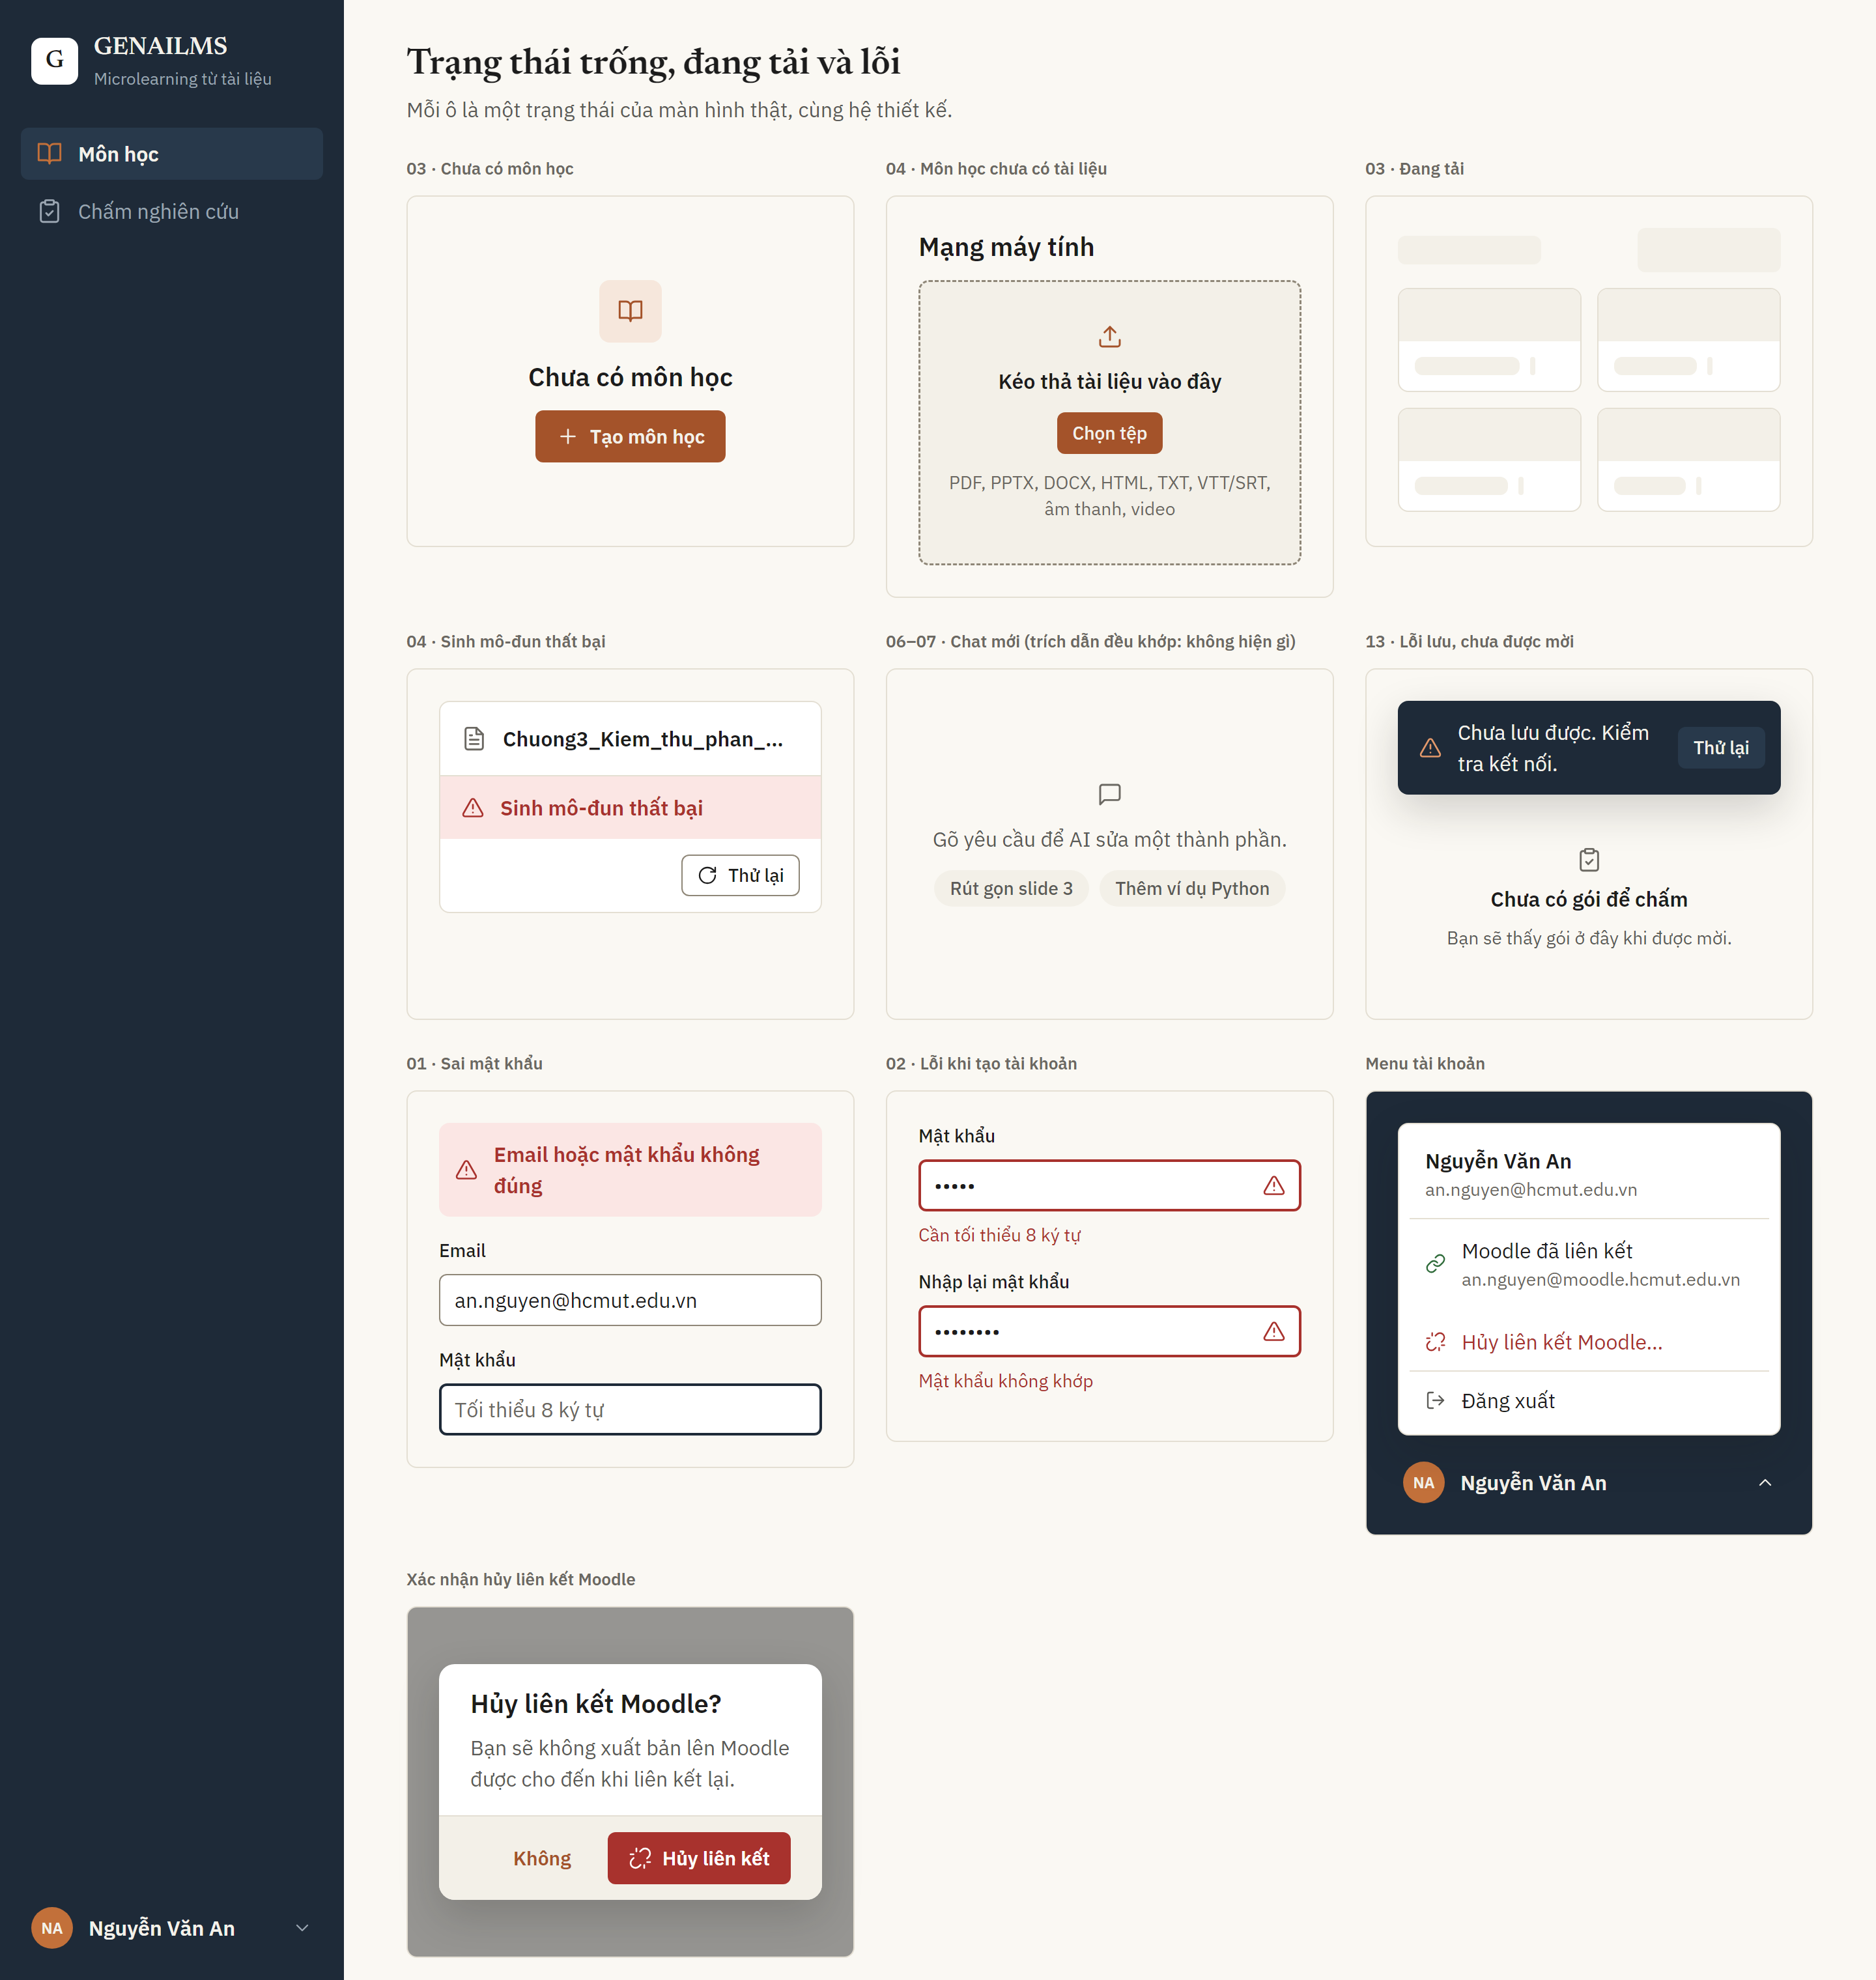
\includegraphics[width=.47\linewidth,height=.26\textheight,keepaspectratio,viewport={620 750 1320 1380},clip]{graphics/ui/15-empty-loading-error-states.png}\hfill
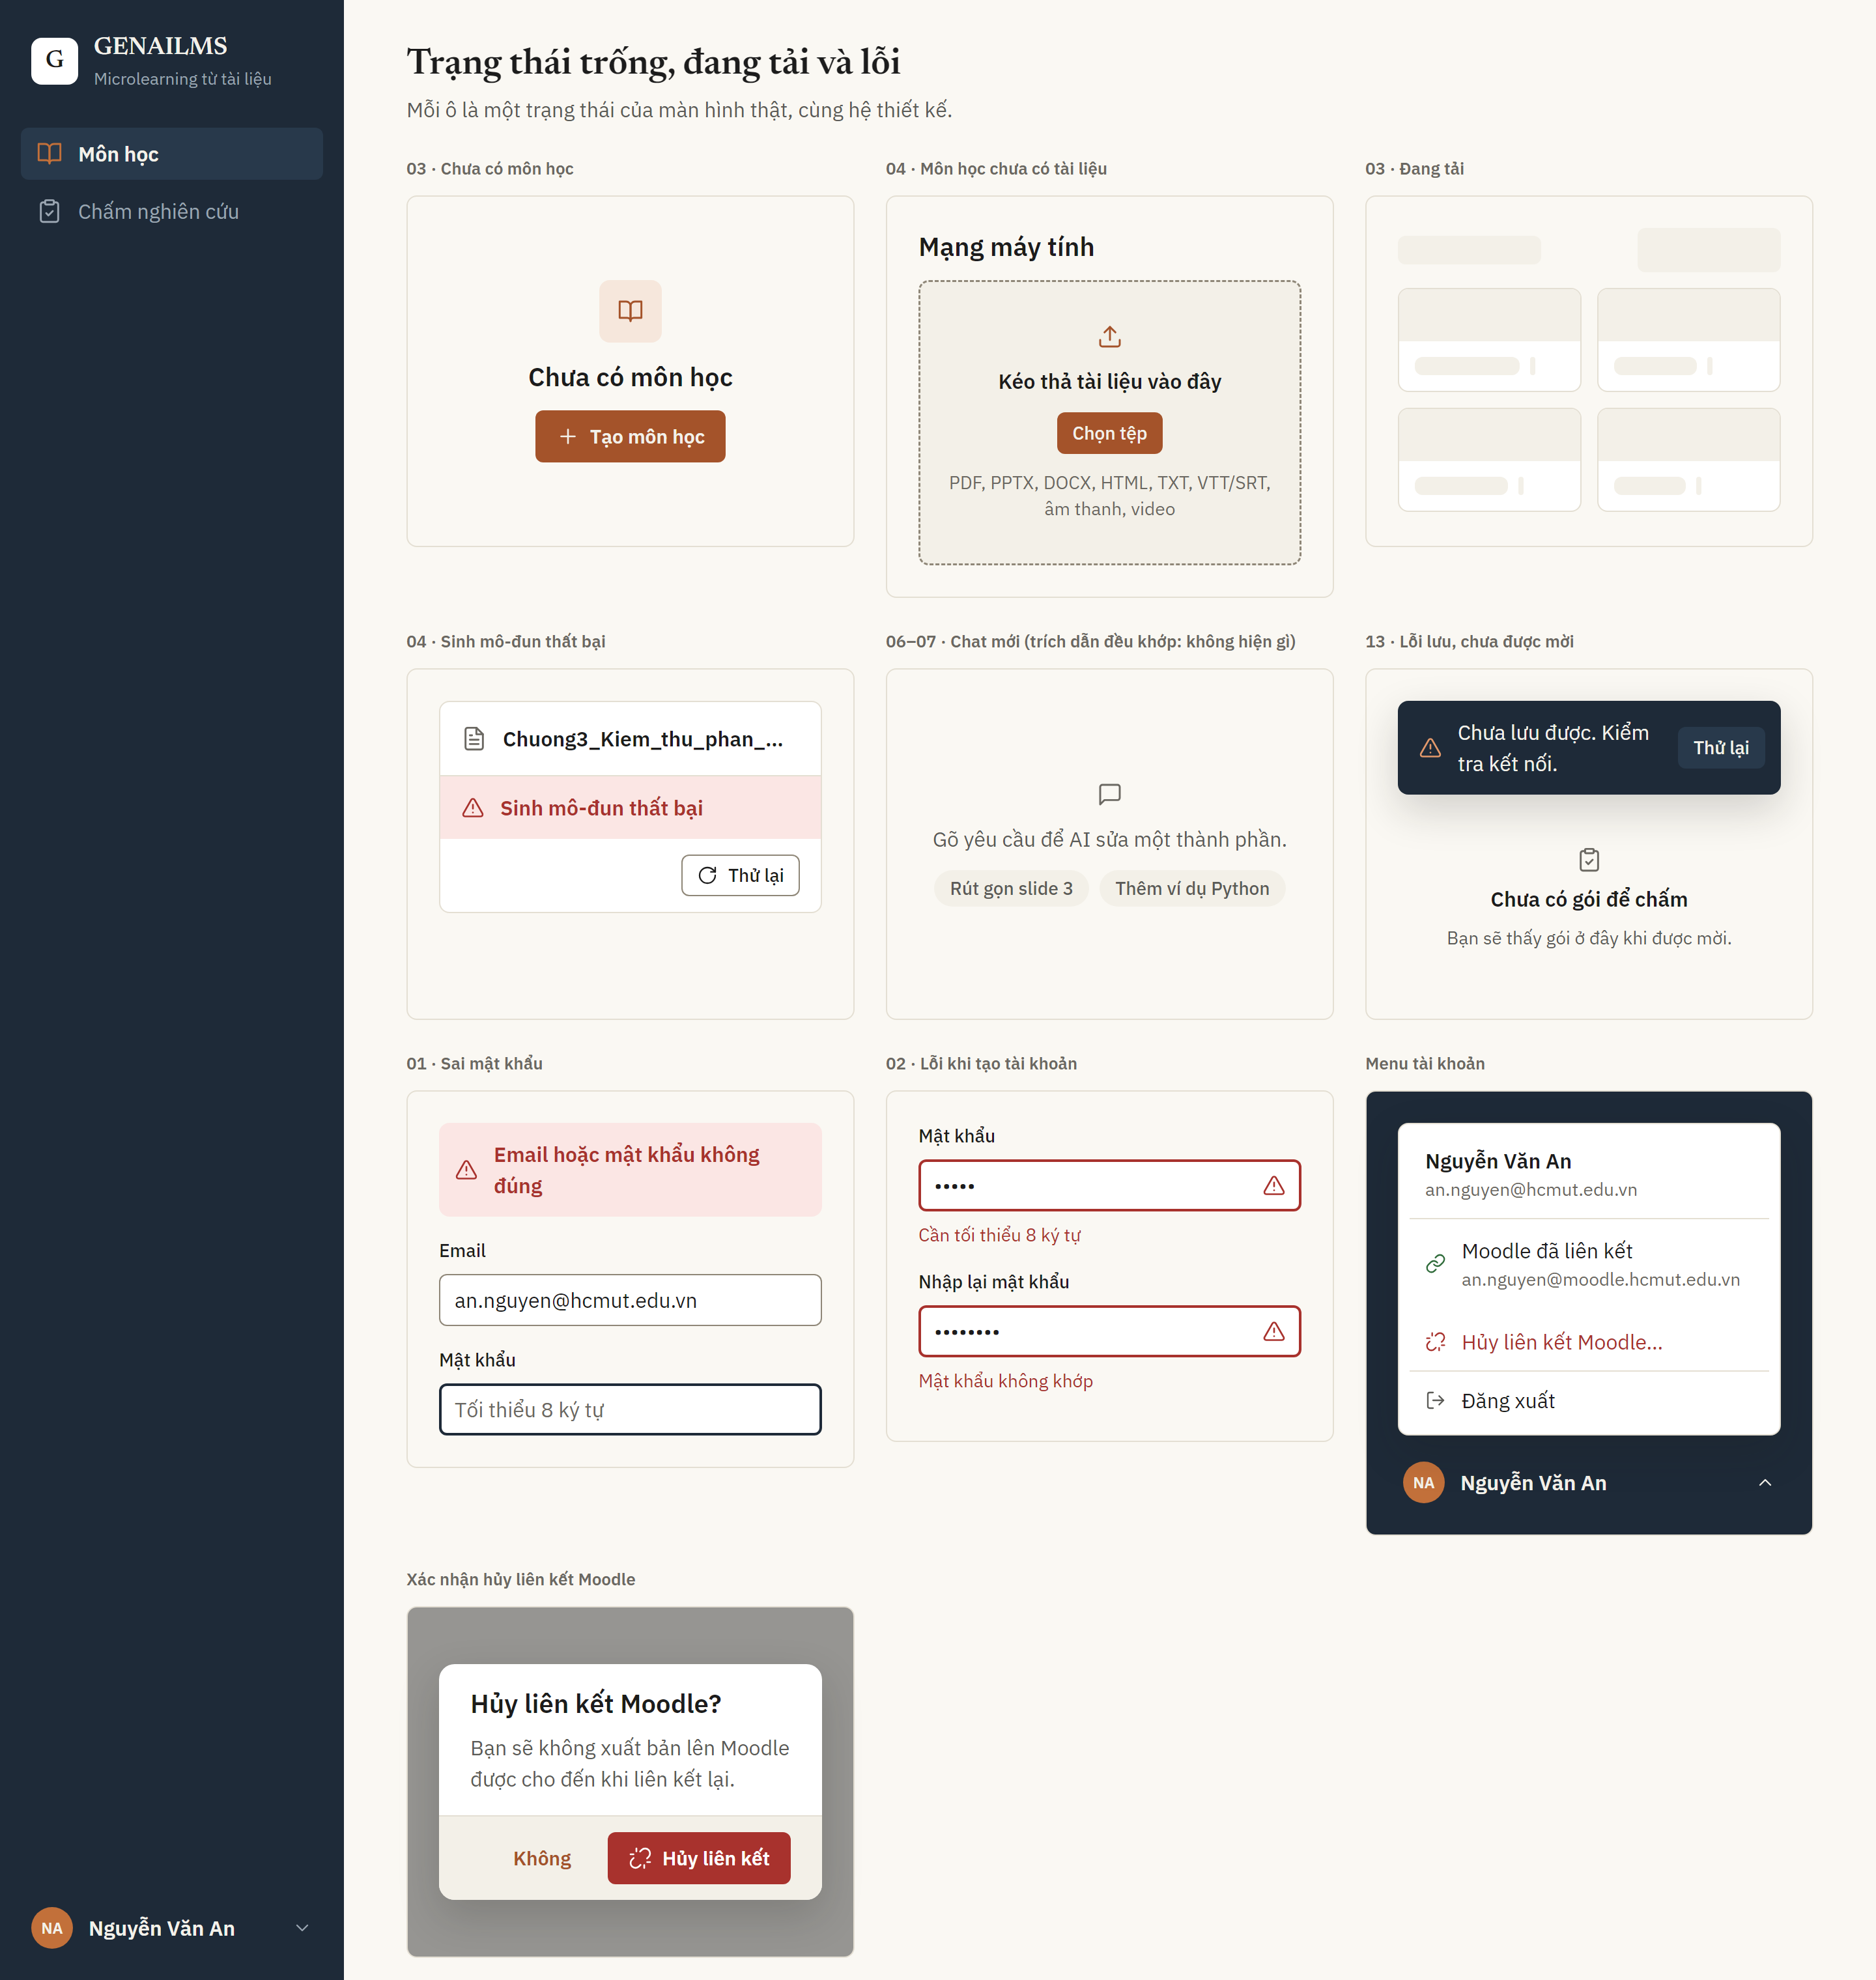
\includegraphics[width=.47\linewidth,height=.26\textheight,keepaspectratio,viewport={1360 790 2050 1380},clip]{graphics/ui/15-empty-loading-error-states.png}\par\smallskip
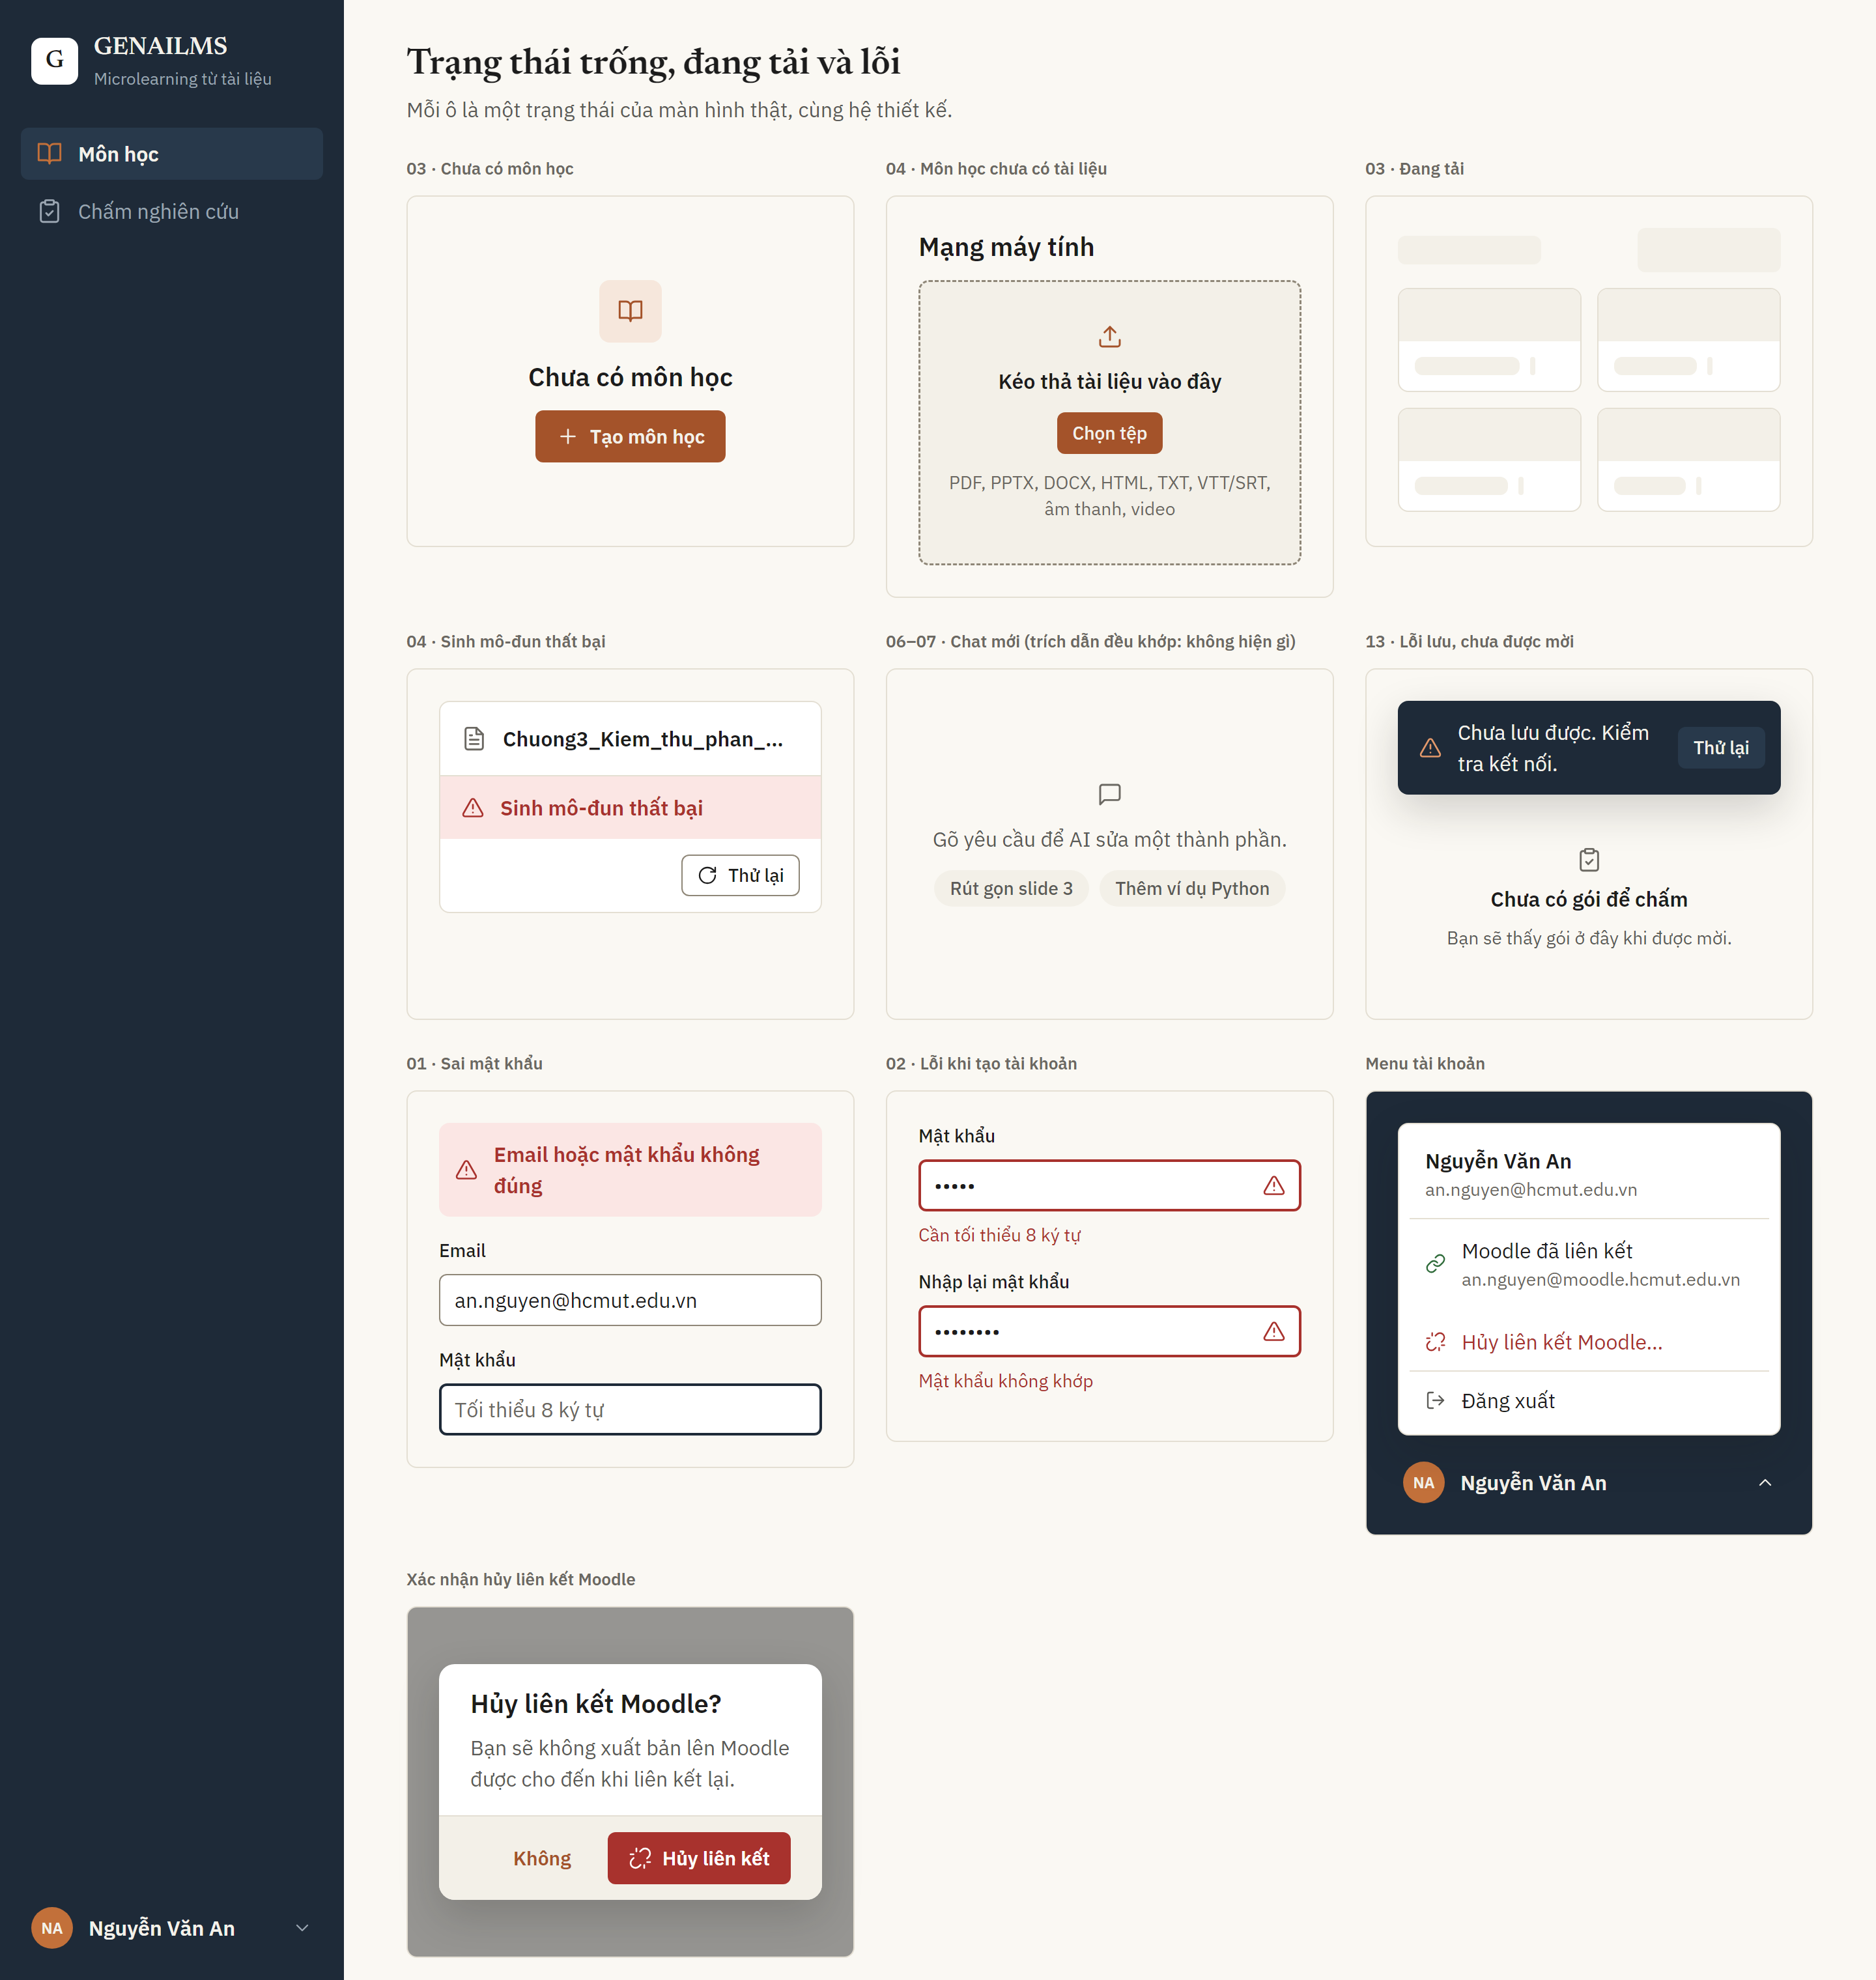
\includegraphics[width=.47\linewidth,height=.26\textheight,keepaspectratio,viewport={2100 640 2800 1380},clip]{graphics/ui/15-empty-loading-error-states.png}\hfill
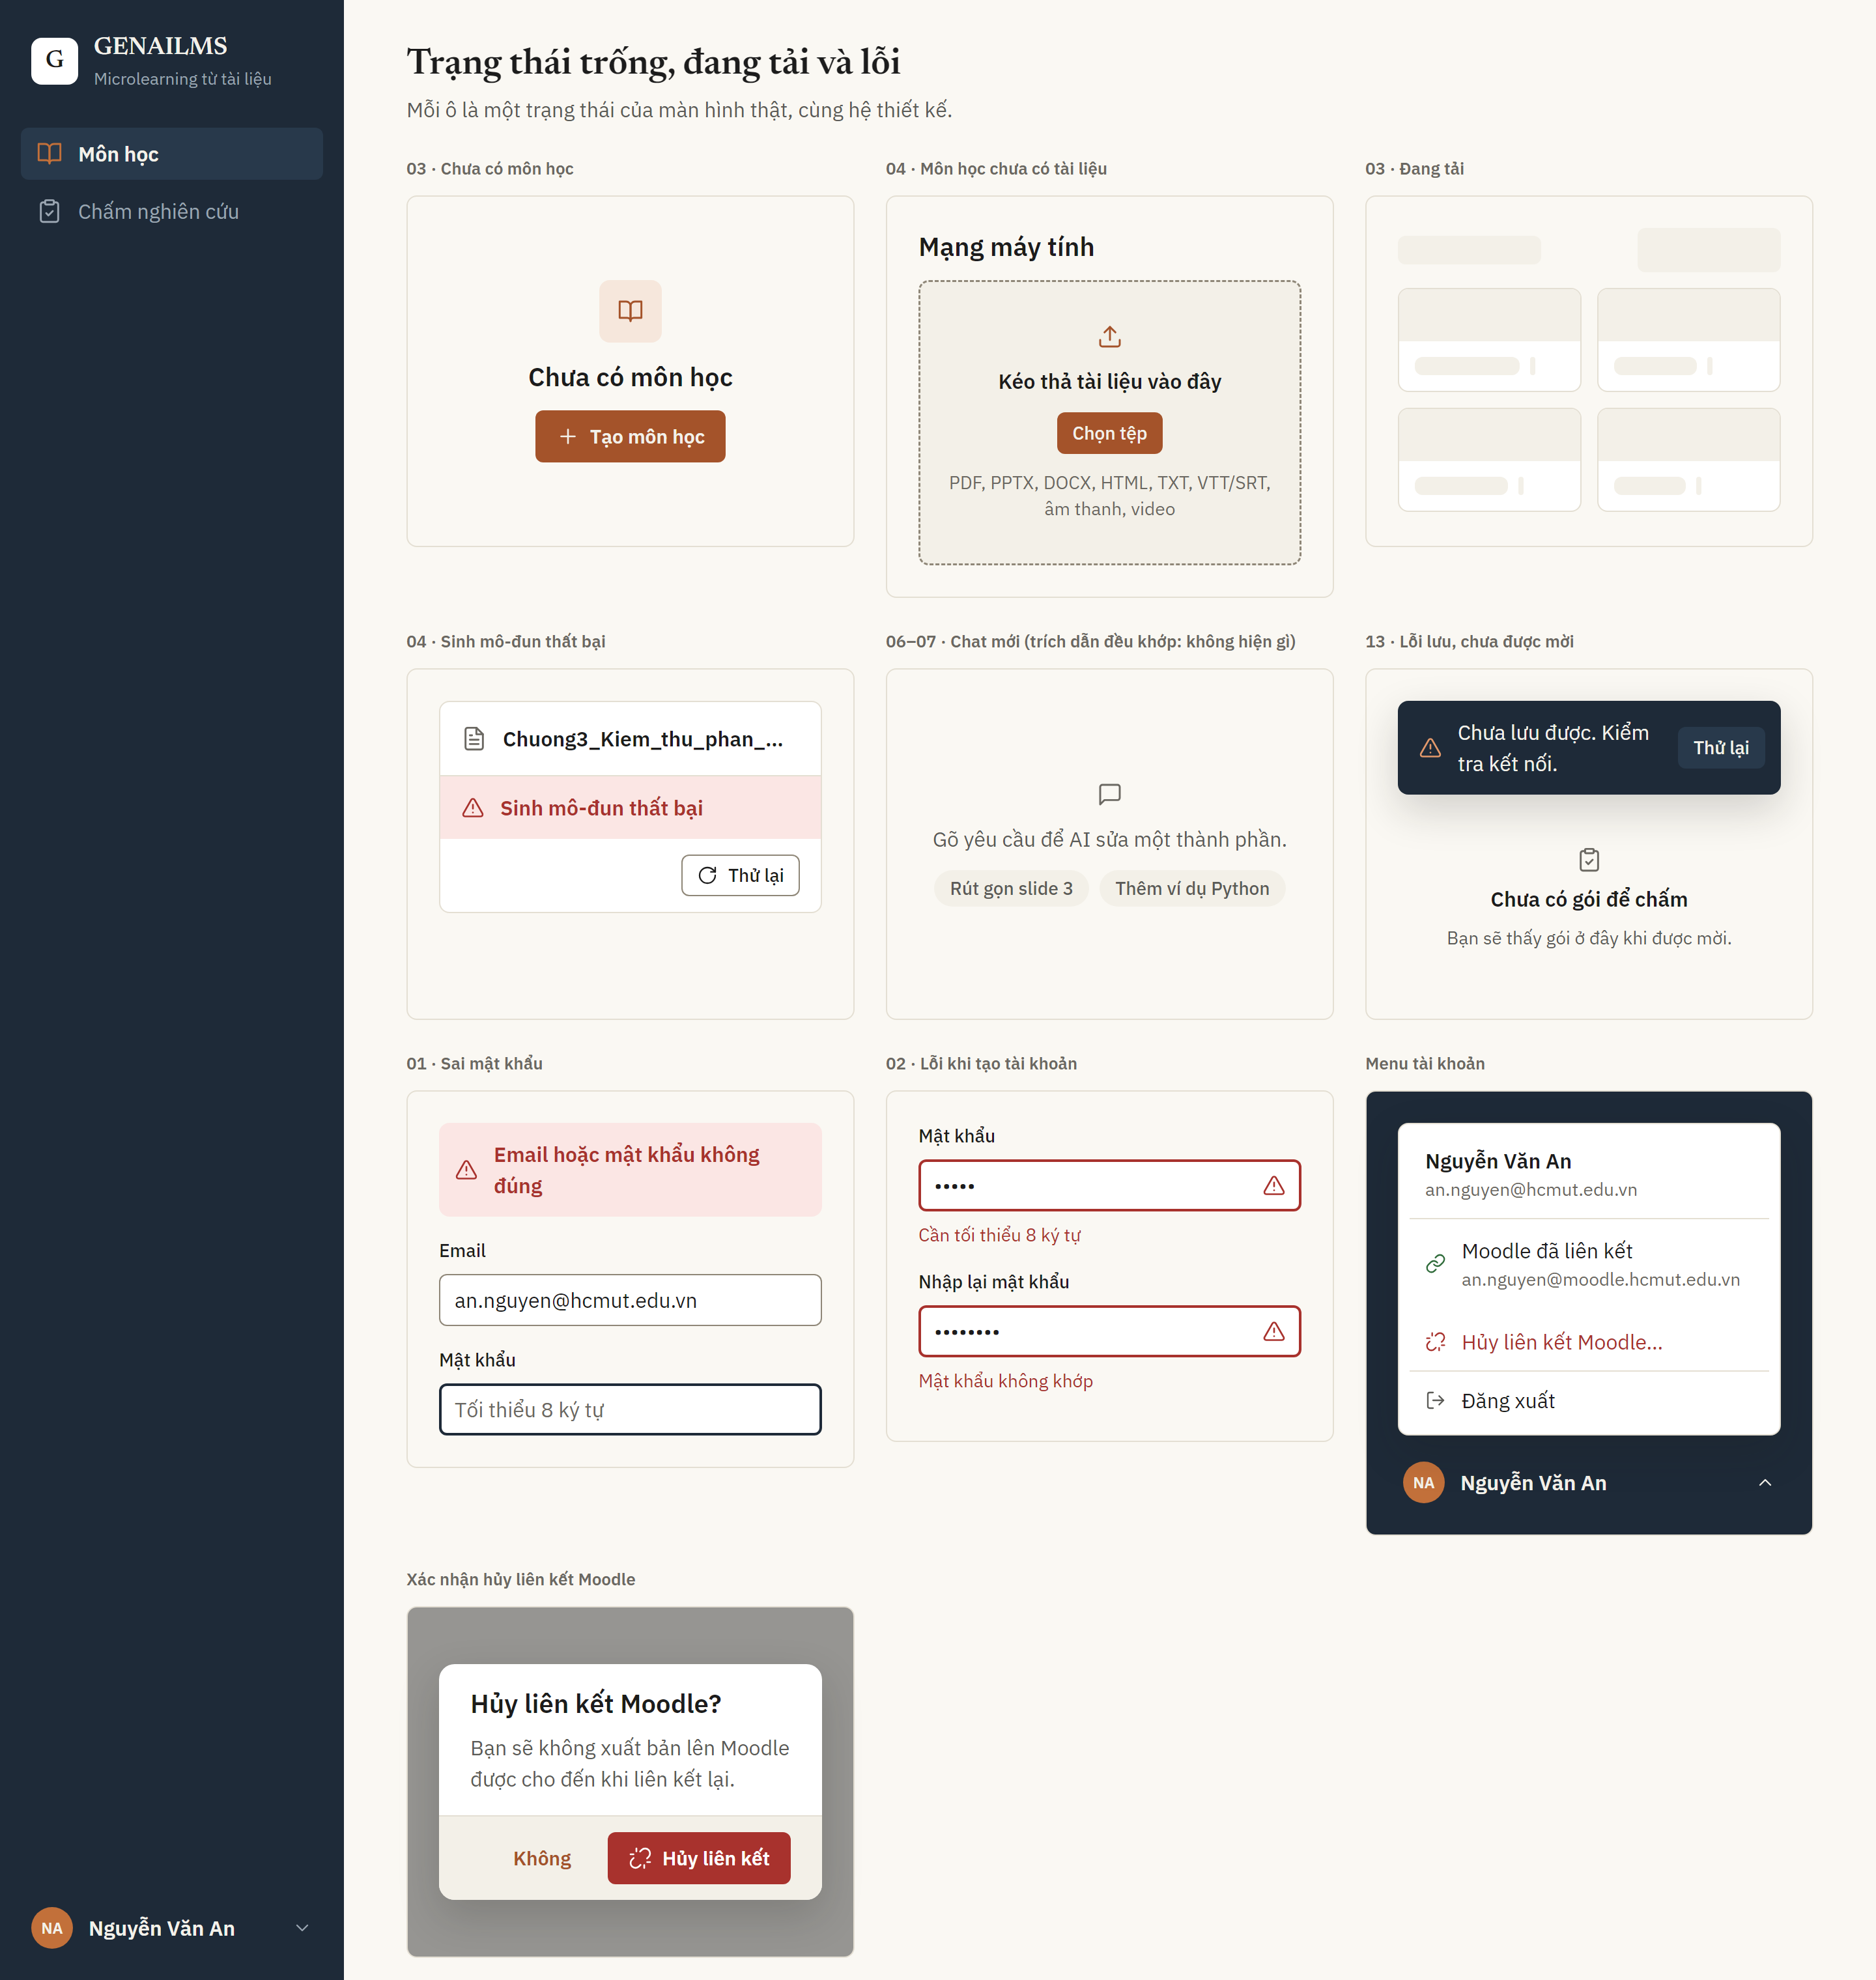
\includegraphics[width=.47\linewidth,height=.26\textheight,keepaspectratio,viewport={620 20 1320 580},clip]{graphics/ui/15-empty-loading-error-states.png}\par\smallskip
\caption{Validation, account menu and unlink confirmation.}\label{fig:ui-screen-15-account}
\end{figure}

\clearpage\section{Evaluation method}\label{sec:evaluation}
This section defines how the system is evaluated. The software for every step is implemented: study setup, blinded rating, model judges, claim extraction and the statistical analysis. What has been run so far is reported in Section~\ref{sec:results}.
\subsection{Questions}
\begin{enumerate}[label=Q\arabic*.,leftmargin=*,nosep]
\item Does retrieval find the passage a question needs, in English, Vietnamese and across the two languages?
\item Are course chat answers supported by the retrieved passages and relevant to the question?
\item Does generation with retrieval reduce unsupported statements in a module while keeping completeness and question quality?
\item Do the citations point to passages that support their statements?
\item Do model judges agree with human raters, and human raters with each other?
\item What latency, resources and cost does the system need, and where does it stop scaling?
\end{enumerate}
\subsection{Retrieval and chat}
Retrieval (Q1) uses questions written by a model from one chunk each, with that chunk as the only correct answer, so Recall@$k$ equals Hit Rate@$K$. MRR@10 and nDCG@10 are reported with it, and paired configurations are compared with exact McNemar tests on rank-one recall\citep{mcnemar}. A cross-language set translates English questions over English material into Vietnamese. Chat (Q2) is scored with Ragas\citep{ragas}: faithfulness is the share of an answer's claims supported by the retrieved contexts, answer relevancy the mean embedding similarity between the question and questions the judge writes for the answer. The judge is of a different model family than the generator\citep{selfpreference}.
\subsection{Module comparison}\label{sec:conditions}
The experimental unit is a pair of modules on the same Learning Objective, generated by the same pipeline and model with the same settings: one with retrieval (\code{rag_llm}) and one without (\code{llm_no_rag}). The control takes its LO from the RAG module and uses the same prompts without the block of source passages, so the two differ only in retrieval. Both are judged against the same reference passages of the document, never against the passages the RAG module chose to cite. Experiment mode pins the model and disables fallback, and the model that served each call is recorded and checked.

The midterm plan is a pilot of 25 pairs and a held-out set of 100 pairs split by document; other conditions (self-check off, retrieval variants, a stronger generator) use matched subsets.
\subsection{Rubric, raters and judges}
Raters score each packet on eight criteria from 1 to 5, each with a reason: accuracy, completeness, consistency, hallucination, slide quality, quiz quality, Bloom fidelity and query alignment, with anchors in \code{docs/rubric.md}. A packet shows only content and an anonymous code, never the group, subject, file or model. Each rater sees the packets in a stable shuffled order and calibrates on two packets outside the sample first. Two model judges, of two families different from the generator's and from each other, score the same packets with the same rubric.
\subsection{Unsupported claims and citations}
The Content of a module is split into atomic claims\citep{factscore}, each checked against the reference passages of its pair. Equation~\ref{eq:unsupported} defines the rate:
\begin{equation}\label{eq:unsupported}
\mathrm{unsupported\_rate}=\frac{\text{unsupported claims}}{\text{assessed claims}}.
\end{equation}
A packet counts only when its reference coverage is complete, i.e. the reference holds every chunk of the document, and at least one claim was extracted. Each citation of a RAG module is checked against the chunk it resolves to\citep{alce}:
\begin{equation}\label{eq:citation}
\mathrm{citation\_accuracy}=\frac{\text{citations whose chunk supports the claim}}{\text{assessed citations}}.
\end{equation}
\subsection{Analysis}
Paired rubric scores are compared with Wilcoxon signed-rank tests\citep{wilcoxon} and Holm correction over the eight criteria\citep{holm}; ``at least one unsupported claim'' is compared with exact McNemar tests. Agreement between two raters uses quadratic weighted kappa\citep{weightedkappa} and Spearman correlation\citep{spearman}; agreement within the group of human raters uses ordinal Krippendorff's $\alpha$\citep{krippendorff}, also with each judge added as one more rater. Intervals are bootstrapped over questions or pairs\citep{bootstrap}.
\subsection{Performance and scalability}
Latency is recorded per stage of every job. Throughput is measured by load tests with k6 and with real models, adding tasks of one service at a time so that one bottleneck does not hide another. A mock model is used only for failure tests and to measure the streaming path, never as evidence of capacity, because it has no provider quota. Failure tests stop each kind of service while it works and check that no job is lost or done twice.

\clearpage\section{Results}\label{sec:results}
This section reports what has been measured by November 2026: retrieval, chat answers, a first pilot of the module quality evaluation (Section~\ref{sec:evaluation}), extraction, latency, resource use, scalability and behaviour when a service fails. The pilot has no human ratings and no judge of the planned pair yet. Each table states its conditions, because most numbers come from one machine and some from a single run.
\subsection{Measurement setup}\label{sec:results-setup}
Unless stated otherwise, measurements ran under WSL2 on an Intel i7-12700H laptop with an RTX 3050 Ti Laptop GPU (4 GB). Docker had 7.57 GiB of memory, and the load generator, database and every service shared this machine. The embedder ran on the GPU; the Jina reranker ran on the CPU with a quota of four cores per container. Language models were reached through the gateway in experiment mode, which disables cross-model fallback and records the served model. Raw results and scripts are kept in \code{docs/measurements}.

The evaluation corpus is the five subjects of \code{docs/documents}: Advanced Programming, Calculus 1, Machine Learning, Operating Systems and Scientific Socialism. It replaces the four computing subjects of the midterm report, so the preliminary benchmarks of Section~\ref{sec:background} are not directly comparable with the results below.
\subsection{Retrieval quality}\label{sec:results-retrieval}
A model wrote 250 questions, 50 per subject, each from one sampled chunk; that chunk is the only one counted as correct. Recall@$k$ is therefore the Hit Rate@$K$ the advisor asked for. Table~\ref{tab:retrieval-5} compares dense search, hybrid search (dense and BM25 fused by reciprocal rank fusion) and hybrid search reranked by Jina.
\begin{table}[H]\centering\small\caption{Retrieval on 250 questions over five subjects.}\label{tab:retrieval-5}
\begin{tabularx}{\linewidth}{|Y|r|r|r|r|r|r|r|}\hline
Configuration & R@1 & R@3 & R@5 & R@8 & R@10 & MRR@10 & nDCG@10\\\hline
Dense & 0.800 & 0.960 & 0.984 & 0.992 & 1.000 & 0.879 & 0.909\\\hline
Hybrid & 0.812 & 0.952 & 0.976 & 0.988 & 0.988 & 0.885 & 0.911\\\hline
Hybrid + Jina rerank & 0.856 & 0.980 & 0.984 & 0.988 & 0.996 & 0.918 & 0.938\\\hline
\end{tabularx}\end{table}
\begin{table}[H]\centering\small\caption{Hybrid + Jina rerank by subject.}\label{tab:retrieval-subject}
\begin{tabularx}{\linewidth}{|Y|r|r|r|r|}\hline
Subject & R@1 & R@8 & MRR@10 & nDCG@10\\\hline
Advanced Programming & 0.800 & 1.000 & 0.893 & 0.921\\\hline
Calculus 1 & 0.760 & 0.980 & 0.857 & 0.892\\\hline
Machine Learning & 0.920 & 1.000 & 0.960 & 0.970\\\hline
Operating Systems & 0.860 & 0.980 & 0.920 & 0.936\\\hline
Scientific Socialism & 0.940 & 0.980 & 0.959 & 0.969\\\hline
\end{tabularx}\end{table}
Exact McNemar tests on rank-one recall found no significant difference: reranked against hybrid 27 against 16 discordant questions ($p=0.126$), reranked against dense 31 against 17 ($p=0.060$), hybrid against dense 18 against 15 ($p=0.728$). In Calculus 1, hybrid search was below dense. These questions are easier than real student questions: each was written from its target chunk in the same language, which is why Recall@10 is close to 1.0.
\subsection{Reranking options}\label{sec:results-rerank}
The hosted Jev reranker was compared with Jina and with no reranking on the same 30 hybrid candidates per question. Fifty questions (every fifth) were used only to choose how to call Jev: one call per chunk ranked better than one call for all candidates (MRR 0.942 against 0.906). The acceptance limits were fixed before the 200 remaining questions were scored: relative to Jina, Recall@8 may drop by at most 0.01 and MRR@10 by at most 0.02, and MRR must exceed no reranking. A Vietnamese set of 126 questions, translated from English questions over English material, tests the cross-language case that failed in October.
\begin{table}[H]\centering\small\caption{Reranking options on held-out questions; p95 is the rerank latency without load.}\label{tab:rerank-options}
\begin{tabularx}{\linewidth}{|p{3.3cm}|Y|r|r|r|r|}\hline
Set & Option & R@1 & R@8 & MRR@10 & p95\\\hline
200 questions & No rerank & 0.795 & 0.990 & 0.877 & --\\\hline
200 questions & Jina & 0.845 & 0.985 & 0.909 & 3.56 s\\\hline
200 questions & Jev & 0.925 & 0.995 & 0.952 & 1.48 s\\\hline
126 Vietnamese & No rerank & 0.683 & 0.952 & 0.787 & --\\\hline
126 Vietnamese & Jina & 0.802 & 0.976 & 0.873 & 2.89 s\\\hline
126 Vietnamese & Jev & 0.873 & 0.976 & 0.918 & 0.46 s\\\hline
\end{tabularx}\end{table}
Paired bootstrap 95\% intervals for Jev minus Jina were $+0.010$ ($-0.010$ to $+0.030$) for Recall@8 and $+0.044$ ($+0.007$ to $+0.080$) for MRR@10 on the 200 questions, and $0.000$ ($-0.024$ to $+0.024$) and $+0.046$ ($-0.008$ to $+0.099$) on the Vietnamese set. Jev met the limits on both sets. On the Vietnamese set the Recall@8 interval is wider than the permitted drop, so equivalence there is not demonstrated.

Neither reranker is perfectly repeatable. Rerunning Jina with identical questions and candidates changed the ranking of 12 of 250 questions; rerunning Jev without its cache changed 6 of 250, by at most two places, with unchanged recall and MRR. Without reranking, cross-language questions lose most: MRR falls from 0.885 to 0.787. This is the reason the design keeps reranking rather than dropping it to remove the bottleneck. Adaptive selection of context with floor eight gave equivalent coverage with Jev scores (0.992 on 250 questions, 8.53 chunks on average) and needed no threshold change.
\subsection{Course chat answers}\label{sec:results-chat}
Fifty questions, every fifth of the retrieval set and ten per subject, were asked the way the chat endpoint answers one turn: 30 hybrid candidates, Jina reranking to eight chunks, and \code{gemini-fast} pinned with the gateway's fallbacks off. Every answer was served by \code{gemini-3.5-flash-lite}, and the chunk each question was written from was among the eight contexts in all 50 and cited in 48. Ragas~0.2.15 scored faithfulness (the share of the answer's claims supported by the contexts) and answer relevancy (mean embedding similarity between the question and three questions the judge writes for the answer). The judge was \code{gpt-oss-120b} through Groq, of another family than the generator; all 50 judgments were served by it. Jev was not used, since it waits for the school's agreement.
\begin{table}[H]\centering\small\caption{Course chat answers, 50 questions, one judge, one run; 95\% bootstrap intervals over questions. Refusals are the answers the judge found noncommittal (relevancy 0); faithfulness is over the others, because Ragas scores ``the material does not cover this'' as an unsupported claim.}\label{tab:chat-ragas}
\begin{tabularx}{\linewidth}{|Y|r|r|l|l|}\hline
Set & $n$ & Refused & Faithfulness & Answer relevancy\\\hline
All & 50 & 4 & 0.967 (0.916--1.000) & 0.725 (0.648--0.788)\\\hline
Advanced Programming & 10 & 1 & 1.000 & 0.744 (0.558--0.871)\\\hline
Calculus 1 & 10 & 0 & 0.900 (0.700--1.000) & 0.743 (0.697--0.792)\\\hline
Machine Learning & 10 & 0 & 1.000 & 0.847 (0.781--0.908)\\\hline
Operating Systems & 10 & 2 & 0.958 (0.875--1.000) & 0.685 (0.439--0.888)\\\hline
Scientific Socialism & 10 & 1 & 0.978 (0.933--1.000) & 0.604 (0.432--0.725)\\\hline
\end{tabularx}\end{table}
Four answers said the material did not cover the question although the source chunk was in the context. Two of these were wrong: the code was there and the answer followed from it. The other two asked for a calculation the material only poses and for a topic the chunk only names. The one zero-faithfulness answer replaced each radical sign of a calculus result with other characters. The prompt had forbidden any inference, which also forbade reading code in a source; it now forbids outside information but allows reasoning on the sources and asks for formulas to be copied symbol by symbol. Three out-of-scope questions were still refused. On the same 50 questions and judge, refusals fell to two, faithfulness stayed at 0.966 (0.920--0.995), the integral scored 1.0, and relevancy rose to 0.755, a paired difference of $+0.030$ ($-0.007$ to $+0.076$) that is not significant. Because each question was written from a chunk that was always retrieved, these scores are an upper bound for single-passage questions; the relevancy of the Vietnamese subject may also be lowered by Ragas's English prompts.

\subsection{Generated modules: first pilot}\label{sec:results-modules}
Ten RAG/control pairs were generated, two documents per subject, to exercise the evaluation of Section~\ref{sec:evaluation} end to end with a free model. Each pair is a module generated with retrieval and a module generated by the same pipeline without it, on the same Learning Objective, with self-check on. The generator was \code{gemini-fast} in experiment mode; all 286 model calls of the 20 modules were served by \code{gemini-3.5-flash-lite}, 14 to 19 per RAG module and 12 to 16 per control. A module took 49.5 s on average and 90 s at most, without the time spent waiting for rate limits. The planner cache of these documents, written earlier by Claude Haiku, was cleared so that every step came from the compared model. One document had lost its stored text and was read again from its source file in the backend image; reading another file the same way reproduced its stored text exactly. These documents were not drawn from a held-out split, and ten pairs are fewer than the 25 of the planned pilot, so the results below test the procedure and give a first indication, not the comparison of the thesis. The 20 blinded packets, the scripts and the raw results are in \code{docs/measurements/module-study}.

The unsupported-claim rate of Equation~\ref{eq:unsupported} was measured with \code{gpt-oss-120b} through Groq, of another family than the generator: the Content of each module was split into claims and each claim was checked against the reference passages shared by the pair, and each citation of a RAG module against the chunk it resolves to. All 20 packets were served by that model, in about 370 calls. Three pairs were excluded under the coverage rule of Section~\ref{sec:evaluation}: the two Machine Learning lectures exceed the reference budget, so their eight passages were retrieved and their coverage is unknown, and no claim was extracted from one Calculus control whose Content is mostly LaTeX, which is a failure of extraction rather than a module without claims.
\begin{table}[H]\centering\small\caption{Unsupported claims in module Content, seven pairs with complete reference coverage, one judge.}\label{tab:module-claims}
\begin{tabularx}{\linewidth}{|Y|r|r|}\hline
Measure & RAG & Control (no retrieval)\\\hline
Claims assessed & 120 & 101\\\hline
Unsupported claims & 0 & 17 (16.8\%)\\\hline
Modules with at least one unsupported claim & 0 of 7 & 6 of 7\\\hline
Citations pointing to a supporting chunk (all ten RAG modules) & 148 of 166 (0.892) & --\\\hline
\end{tabularx}\end{table}
The control's rate was higher in six pairs and equal in one (Wilcoxon signed-rank $p=0.031$; exact McNemar on ``at least one unsupported claim'', six discordant pairs against none, $p=0.031$). Reading the flagged claims qualifies what ``unsupported'' means: most are general knowledge and usually true, but absent from the lecturer's material, such as a graphical interface having windows and menus where the slide lists icons, mouse and keyboard; a few judgments are strict. The measure is therefore whether a module stays within the course material, which retrieval achieved here. The incorrect citations, concentrated in three modules, attach a supported statement to a neighbouring chunk.

The rubric of Section~\ref{sec:evaluation} needs two judges from families other than the generator's. Of the planned pool, Claude and GPT-6.1 had no funded key, Gemini is the generator's family, and the Groq account could reach Qwen but not Llama or MiniMax. All 20 packets were therefore scored by \code{qwen3.8-27b} alone, kept in a file separate from the planned run (Table~\ref{tab:module-rubric}).
\begin{table}[H]\centering\small\caption{Rubric means over ten pairs from one preliminary judge, \code{qwen3.8-27b}.}\label{tab:module-rubric}
\begin{tabularx}{\linewidth}{|Y|r|r|r|}\hline
Criterion & RAG & Control & RAG higher / lower / equal\\\hline
Accuracy & 5.0 & 5.0 & 0 / 0 / 10\\\hline
Completeness & 4.5 & 4.2 & 3 / 0 / 7\\\hline
Consistency & 5.0 & 5.0 & 0 / 0 / 10\\\hline
Hallucination & 5.0 & 5.0 & 0 / 0 / 10\\\hline
Slide quality & 4.7 & 5.0 & 0 / 3 / 7\\\hline
Quiz quality & 4.2 & 4.2 & 2 / 2 / 6\\\hline
Bloom fidelity & 4.7 & 4.7 & 1 / 1 / 8\\\hline
Query alignment & 4.6 & 4.9 & 0 / 2 / 8\\\hline
\end{tabularx}\end{table}
No criterion differed (every Holm-corrected $p=1.0$). This judge gave accuracy, consistency and hallucination their maximum in every packet and listed no hallucination, including in the controls where the claim check found 17 unsupported claims. It does not separate the groups, so these scores are not used as evidence. The run shows that a small judge saturates on this rubric, which is the reason the planned judges are the providers' larger models.

\subsection{Document extraction}\label{sec:results-extraction}
The five-subject corpus produced 937 chunks from 23 files, with 375 s of reading and 28 s of embedding when files were processed one after another (Table~\ref{tab:ingest-5}). Calculus 1 is slowest because pages with broken formulas are re-read by a vision model on a free tier, and its time includes waiting for that rate limit. Machine Learning includes lecture recordings, whose time depends on the transcription provider.
\begin{table}[H]\centering\small\caption{Ingestion of the five-subject corpus.}\label{tab:ingest-5}
\begin{tabularx}{\linewidth}{|Y|r|r|r|r|}\hline
Subject & Files & Chunks & Read per file (s) & Embed per chunk (ms)\\\hline
Advanced Programming & 5 & 74 & 1.9 & 33\\\hline
Calculus 1 & 6 & 292 & 46.2 & 35\\\hline
Machine Learning & 4 & 349 & 9.4 & 21\\\hline
Operating Systems & 5 & 147 & 8.5 & 37\\\hline
Scientific Socialism & 3 & 75 & 2.8 & 31\\\hline
\end{tabularx}\end{table}
The Calculus PDFs are TeX slides whose math fonts have no Unicode map, so integrals, radicals and number sets came out as stray letters. Their codes are now mapped and radicals rebuilt from glyph positions; a page still suspect is re-read by a vision model, and the result is kept only when at least 90\% of the text-layer words survive and at most 10\% are new. Of 62 flagged pages, 56 were accepted and 6 kept the rebuilt text with a warning to the lecturer. Text in pictures and SmartArt is now read with Tesseract (\code{vie+eng}), adding 5 to 17 figure blocks per Operating Systems file without a model call. Recordings are transcribed in 600-second windows, which cut the processing time of four recordings by 4.4 to 6.8 times. The strategy for formulas and figures is therefore: deterministic repair first, a vision model only for pages still broken, OCR for figure text, and a visible warning when a result cannot be verified. Diagrams without text are still lost.
\subsection{Generation latency and token use}\label{sec:results-latency}
Nine modules were generated with Claude Haiku 5.5 on the five-subject corpus, five one at a time and four concurrently. All 228 model records were served by Haiku, with no fallback, and all nine modules succeeded.
\begin{table}[H]\centering\small\caption{Module generation with Claude Haiku 5.5.}\label{tab:gen-latency}
\begin{tabularx}{\linewidth}{|Y|r|r|}\hline
Measure & One at a time ($n=5$) & Four concurrent ($n=4$)\\\hline
Module time, mean & 368.9 s & 315.1 s\\\hline
Module time, maximum & 429.3 s & 345.9 s\\\hline
Modules per hour & 9.76 & 41.63\\\hline
Model call, mean / p95 & 13.5 s / 19.7 s & 11.1 s / 17.0 s\\\hline
Rerank, mean / p95 & 2.0 s / 3.6 s & 4.7 s / 9.3 s\\\hline
Prompt / completion tokens per module & 207,810 / 70,444 & 188,795 / 58,459\\\hline
\end{tabularx}\end{table}
Questions took 275.6 s of the 368.9 s, about 75\%, with 17 model calls, which led to generating questions concurrently in every later measurement. Within one retrieval, embedding the query took 0.09 s, BM25 0.006 s, vector search 0.01 s and reranking 2.0 s. Peak memory was 1.0 GiB for the reranker, 565 MiB for the embedder, 387 MiB for the gateway and 65 MiB for PostgreSQL; the GPU used at most 1,283 MiB. A module used about 240,000 tokens with Haiku and about 115,000 with GPT-6 Luna; the cause of the difference has not been established.
\subsection{Scalability}\label{sec:results-scale}
\subsubsection{API reads}
k6 ran 200 virtual users without think time for 60 s, three requests per iteration, after the concurrency-limit fix of Section~\ref{sec:architecture}.
\begin{table}[H]\centering\small\caption{API read throughput by number of API containers.}\label{tab:api-scale}
\begin{tabularx}{\linewidth}{|Y|r|r|r|r|}\hline
API containers & Requests/s & Median & p95 & Failures\\\hline
1 & 199 & 2.9 s & 3.4 s & 0\%\\\hline
2 & 372 & 1.4 s & 1.7 s & 0\%\\\hline
4 & 583 & 0.8 s & 1.2 s & 0\%\\\hline
\end{tabularx}\end{table}
Four containers gave 2.9 times the throughput of one, on a machine that also ran the load generator and the database.
\subsubsection{Module generation with real models}
Table~\ref{tab:gen-scale} shows generation with real models. Each module was generated from its own copy of one lecture (Operating Systems, chapter 3, 33 chunks); $N\times4$ means $N$ workers with four concurrent jobs each, and all jobs were queued at once. A mock language model is not used as evidence of capacity, because it has no provider quota.
\begin{longtable}{|l|l|l|r|r|r|r|r|}\caption{Module generation with real models; Mean and p95 are rerank times, Restarts counts jobs sent back to the queue.}\label{tab:gen-scale}\\\hline
Workers & Model & Rerank & Done & Mod./h & Restarts & Mean & p95\\\hline\endfirsthead
\hline Workers & Model & Rerank & Done & Mod./h & Restarts & Mean & p95\\\hline\endhead
$1\times4$ & Haiku & Jina & 4/4 & 74.9 & 0 & 6.9 s & --\\\hline
$2\times4$ & Haiku & Jina & 7/8 & 28.0 & 17 & 6.2 s & --\\\hline
$4\times4$ & Haiku & Jina & 11/16 & 29.8 & 32 & 21.3 s & --\\\hline
$1\times4$ & Luna & Jina & 4/4 & 90.4 & 0 & 5.1 s & 10.2 s\\\hline
$2\times4$ & Luna & Jina & 8/8 & 107.7 & 0 & 12.0 s & 23.8 s\\\hline
$4\times4$ & Luna & Jina & 16/16 & 162.4 & 0 & 32.4 s & 48.3 s\\\hline
$8\times4$ & Luna & Jina & 32/32 & 182.5 & 0 & 80.8 s & 123.5 s\\\hline
$4\times4$ & Luna & Jev & 16/16 & 319.3 & 0 & 0.9 s & 1.25 s\\\hline
$8\times4$, run 1 & Luna & Jev & 32/32 & 637.7 & 0 & 0.9 s & 1.38 s\\\hline
$8\times4$, run 2 & Luna & Jev & 32/32 & 336.0 & 0 & 1.3 s & 2.74 s\\\hline
$8\times4$, run 3 & Luna & Jev & 32/32 & 539.1 & 0 & 1.1 s & 1.83 s\\\hline
\end{longtable}
With Jina, throughput levelled off because rerank time grew from 5 s to 81 s while model latency stayed near 12 s. Haiku failed differently: its provider rate limit caused a cascade of retries from two workers upward, with a ceiling estimated at about 87 modules per hour from its 80,000 output tokens per minute. With Jev, rerank stayed near 1 s and eight workers reached 336 to 638 modules per hour (504 on average). In those runs 32 jobs filled exactly 32 slots, so they measure a burst, not sustained capacity. Repeated runs of the same configuration varied widely: four $4\times4$ runs with Luna and Jina ranged from 108.8 to 180.7 modules per hour, so adding a second reranker, embedder or gateway showed no effect that can be separated from this variation. A run with 96 queued modules was cut short when the model credit ran out; before that, 58 modules finished in about 5.5 minutes, about 630 per hour, with no job restarted.
\subsubsection{Course chat}
Table~\ref{tab:chat-scale} measures complete answers before chat streamed, with Luna and one reranker. With Jina, chat stayed at 22.5 messages per minute however many API tasks were added, while the reranker used about 350\% CPU and the API 1--2\%.
\begin{table}[H]\centering\small\caption{Chat throughput before streaming, by number of API tasks.}\label{tab:chat-scale}
\begin{tabularx}{\linewidth}{|r|r|r|Y|r|Y|}\hline
API & Messages & Jina msg/min & Jina mean, p95 & Jev msg/min & Jev mean, p95\\\hline
1 & 50 & 22.4 & 53.0 s, 71.2 s & 151.6 & 8.7 s, 11.0 s\\\hline
2 & 100 & 22.5 & 97.7 s, 132.9 s & 280.6 & 9.2 s, 11.7 s\\\hline
4 & 200 & 22.5 & 164.9 s, 239.1 s & 462.3 & 10.8 s, 13.4 s\\\hline
\end{tabularx}\end{table}
With Jina, 5 of 100 and 60 of 200 messages received HTTP 503; with Jev there were none. The streaming path was then measured with real Jev and a mock model that sends its first word after 1.5 s and finishes after 6 s, so it measures the system and not a model (Table~\ref{tab:chat-sse}). One API task handled four new messages per second with a first-word p95 near 2.1 s and saturated at eight; two tasks handled eight per second at 2.56 s.
\begin{table}[H]\centering\small\caption{Streaming chat with real Jev and a mock model.}\label{tab:chat-sse}
\begin{tabularx}{\linewidth}{|r|r|r|Y|}\hline
API tasks & New messages/s & Messages/min handled & First word, p95\\\hline
1 & 1 & 52.0 & 2.20 s\\\hline
1 & 2 & 102.8 & 2.04 s\\\hline
1 & 4 & 204.3 & 2.14 s\\\hline
1 & 8 & 305.5 & 15.74 s\\\hline
2 & 8 & 407.4 & 2.56 s\\\hline
4 & 8 & 407.8 & 2.23 s\\\hline
4 & 16 & 251.8 & 97.9 s\\\hline
\end{tabularx}\end{table}
The drop at four tasks and 16 messages per second matches a limit of Jev measured directly. From one process, Jev served 34.7 to 269.3 calls per second at 8 to 64 concurrent calls with p95 below 0.3 s, held about 278 calls per second for 45 s at 64, and fell to about 60 calls per second from 128 concurrent calls upward, with slow replies and no rejections. The limit of 64 concurrent Jev calls is per process, so several tasks together can exceed it; whether the drop comes from Jev or from the single measuring machine is not known.

In a real browser with Groq \code{gpt-oss-120b} and Jina and no other load, the first word of nine answers appeared after 3.4 to 7.3 s. The run found three faults that mocked tests had missed, all fixed: the input reopened during a stream, citation markers came in unexpected forms, and an English question after Vietnamese turns was answered in Vietnamese.
\subsection{Language-model load control}\label{sec:results-l1}
Thirty-two modules were generated with Groq \code{gpt-oss-120b} at $4\times4$, where the provider's real 429 responses occur (Table~\ref{tab:l0-l1}).
\begin{table}[H]\centering\small\caption{Behaviour under real rate limiting, one run each.}\label{tab:l0-l1}
\begin{tabularx}{\linewidth}{|Y|r|r|r|r|r|}\hline
Configuration & Done & Failed & Modules/h & Job attempts & Calls retried after 429\\\hline
L0, previous behaviour & 1 & 31 & 17.6 & 159 & 0\\\hline
L1, per-call retry & 30 & 2 & 241.2 & 4 & 141\\\hline
\end{tabularx}\end{table}
Under L0 one 429 took the model's only deployment out of service for 60 s, the following calls failed with no deployment available, and each job restarted from the beginning. The two L1 failures came from malformed citation markers, not from load. The evidence is limited: each configuration ran once instead of the planned three times, and the Jev credit ran out during the L1 run, so 165 of 246 reranks fell back to the hybrid order. The difference between 1 and 30 completed modules is large enough to choose L1, but 241.2 is not a sustained capacity. L1 also used about 407,000 tokens per minute while the provider's header announced 250,000, so capacity ceilings calculated from token limits are not verified. When Jev returned ``payment required'', no job failed, but retrieval quality fell without any warning; this led to the fallback log and alarm described in Section~\ref{sec:rerank-choice}.
\subsection{Failure tests}\label{sec:results-failure}
Before S6 on AWS (Table~\ref{tab:aws-experiments}), each kind of service was stopped while it was working on one machine, with \code{devops/loadtest/run_failures.sh}. Postgres, Redis, the embedder, the reranker, two \code{api} and two \code{worker} containers with four job threads each were real; the language model was a mock with a median of 13.3 s per call, so no paid model was used and the times are not capacity figures. Each generation scenario queued eight modules, applied the fault 60 s later and waited for every job. A scenario passes when all eight jobs finish and each document has exactly one module, so no job is lost and none is done twice.
\begin{table}[H]\centering\small\caption{Generation under failure, eight modules per scenario, one run each. Attempts count failed attempts over all jobs and, in brackets, the most for one job; the queue gives up at five.}\label{tab:failure-gen}
\begin{tabularx}{\linewidth}{|p{2.6cm}|Y|r|r|r|r|}\hline
Scenario & Fault & Done & Modules & Attempts & Wall\\\hline
Baseline & None & 8/8 & 8 & 0 (0) & 240 s\\\hline
Worker stop & \code{docker stop} of one worker, as a deployment or scale-in does & 8/8 & 8 & 0 (0) & 258 s\\\hline
Worker kill & \code{kill -9} of one worker, restarted 5 s later & 8/8 & 8 & 4 (1) & 1,090 s\\\hline
Gateway & LLM gateway stopped for 60 s & 8/8 & 8 & 22 (3) & 342 s\\\hline
Reranker & Reranker stopped for 60 s & 8/8 & 8 & 6 (1) & 342 s\\\hline
Embedder & Embedder stopped for 60 s & 8/8 & 8 & 8 (2) & 321 s\\\hline
Database & \code{docker compose restart db} & 8/8 & 8 & 2 (1) & 255 s\\\hline
API kill & \code{kill -9} of one \code{api} container & 8/8 & 8 & 0 (0) & 238 s\\\hline
\end{tabularx}\end{table}
All eight scenarios passed. A stopped worker returned its four jobs to the queue, and the other worker took them without counting an attempt. A killed worker lost no job, but its four jobs stayed running until the sweeper's 15-minute threshold and were requeued 14 minutes after the kill, which accounts for the 1,090 s. A 60 s gateway outage already took one job to three of its five attempts. Killing an \code{api} container changed nothing, because the API is not on the generation path.

Chat was tested with six messages, two at a time, while one dependency was stopped. With Redis stopped, all six answered, because rate limits fall back to each process. With the reranker stopped, all six failed with HTTP 500: the non-streaming endpoint searched through the generation path, which retries the reranker five times and then raises, and only the streaming endpoint had the chat fallback. With the embedder stopped, two of six failed; the other four were served from the query-embedding cache. Both endpoints now share one chat search, which keeps the hybrid order when reranking fails and uses BM25 alone when the question cannot be embedded; after the fix all six answered in each case, the embedder case with a cold cache.

The runs led to two changes in recovery, described in Section~\ref{sec:architecture}: the sweeper threshold fell from 15 to 5 minutes, and errors from an unavailable dependency back off from 30 s instead of 5 s. Only the two affected scenarios were run again (Table~\ref{tab:failure-after}).
\begin{table}[H]\centering\small\caption{The two scenarios rerun after the recovery changes.}\label{tab:failure-after}
\begin{tabularx}{\linewidth}{|p{2.6cm}|Y|Y|}\hline
Scenario & Before & After\\\hline
Worker kill & Requeued 14 min 11 s after the kill; wall 1,090 s & Requeued 4 min 10 s after the kill; wall 505 s\\\hline
Gateway, 60 s & 22 attempts, at most 3 of 5 for one job; wall 342 s & 13 attempts, at most 2 of 5; wall 369 s\\\hline
\end{tabularx}\end{table}
Five missed beats are still required, so a live job is never requeued; a beat that fails is retried after 5 s, so a worker whose database connection was cut refreshes its locks as soon as the database returns. The gateway scenario took 27 s longer, because a job now waits longer before its first retry after a short outage. These are single runs on one machine with a mock model. They do not cover a Valkey or PostgreSQL outage longer than a restart, a network partition, a full disk, Moodle stopping during publication, or ECS replacing tasks on AWS.

Both roles were then followed in a real browser through Moodle 5.2 and the LTI activity (\code{devops/browser-e2e}). The teacher uploaded a chapter, ready in 30 s, and chatted with it; the student reached the chat page, was sent back to it from author pages and found the conversation after a reload. One fault was found: a document whose embedding failed because the embedder was stopped showed the lecturer a raw exception. Such a job is now marked as a system failure, and the lecturer is told to retry later while the exception stays in the job for the administrator.
\subsection{What the results support}
The results support five design decisions: keep reranking, because cross-language questions need it; treat CPU reranking as the bottleneck to remove; retry rate-limited calls individually instead of restarting jobs; stream chat from the API tasks; and let chat answer with reduced retrieval when a search dependency fails, while generation waits and retries. The module pilot gives a first indication that retrieval keeps module content within the course material, from one claim judge on seven pairs; the rubric comparison and agreement with human raters remain to be measured. The failure tests show that no job is lost or done twice when a single service fails on one machine. They do not yet support claims of sustained capacity, recovery on AWS, or any number on AWS. Those are listed with what each needs in Section~\ref{sec:progress}.

\clearpage\section{Conclusion and future work}\label{sec:conclusion}\label{sec:plan}\label{sec:progress}
\subsection{Summary}
GENAILMS is implemented end to end: a lecturer uploads course documents, generates a seven-part module with a citation to the exact passage behind each important statement, reviews and edits it, and publishes it to Moodle as a Book and quizzes. Lecturers and students open it from Moodle through LTI 1.3; students can only chat over their course's material and lose access within about an hour of leaving the Moodle course. The system runs as stateless services with the data, vectors and job queue in PostgreSQL, and its AWS deployment is written in Terraform. On 7 November 2026, 1,566 backend tests and 273 frontend tests pass in continuous integration.

The main results on the five-subject corpus are:
\begin{itemize}[leftmargin=*,nosep]
\item Retrieval with hybrid search and Jina reranking reached Hit Rate@1 0.856, MRR@10 0.918 and nDCG@10 0.938 on 250 questions. The hosted Jev reranker ranked at least as well (MRR@10 0.952 against 0.909 on 200 held-out questions) with a p95 rerank time 2.4 to 6.3 times lower.
\item Course chat answers had a faithfulness of 0.966 and an answer relevancy of 0.755 on 50 questions, after a prompt change that removed both wrong refusals.
\item In a pilot of ten module pairs, Content generated with retrieval had no unsupported claim (0 of 120), against 17 of 101 without retrieval ($p=0.031$, seven pairs), and 89\% of citations pointed to a supporting chunk.
\item CPU reranking was the shared bottleneck of generation and chat; with the hosted reranker, chat went from 22.5 to 462 messages per minute on four API tasks and generation reached 336 to 638 modules per hour in bursts. Retrying rate-limited calls one by one raised completed modules from 1 to 30 of 32 under real provider limits.
\item No job was lost or done twice when any single service was stopped or killed on one machine.
\end{itemize}
\subsection{Status against the advisor's targets}
\begin{longtable}{|p{3.2cm}|p{6.2cm}|p{4.4cm}|}\caption{Advisor targets and their state.}\label{tab:feedback}\\\hline
Target & Done & Remaining\\\hline\endfirsthead
\hline Target & Done & Remaining\\\hline\endhead
Five-subject corpus & 23 files, 937 chunks, 250 retrieval questions & Real student questions\\\hline
Hit Rate@$K$, MRR, nDCG & Three configurations, two rerankers, a cross-language set (Section~\ref{sec:results-retrieval}) & Human labels allowing several correct chunks\\\hline
Faithfulness, answer relevance & Ragas on 50 chat answers (Section~\ref{sec:results-chat}); unsupported claims and citation accuracy on a ten-pair module pilot (Section~\ref{sec:results-modules}) & Held-out pairs; a second claim judge\\\hline
Latency and resources & Per stage and under load (Sections~\ref{sec:results-latency} and~\ref{sec:results-scale}) & Chat time to first word under load with a real model; any number on AWS\\\hline
Inter-rater reliability & Kappa, Krippendorff's $\alpha$ and Spearman analysis; blind rating screens and a rater kit; 20 pilot packets ready & Human raters; the two planned judges\\\hline
Figures and code in documents & Formula repair, vision re-reading of broken pages, figure OCR, SmartArt text (Section~\ref{sec:results-extraction}) & Diagrams without text; fidelity of code\\\hline
AWS within \$200, lock-in & Terraform, deployment script, cost estimate, lock-in analysis (Section~\ref{sec:aws}); a first apply on a real account & A complete apply after account verification, and S1--S8\\\hline
Scalability & Stateless services; bottlenecks measured and removed; failure tests (Section~\ref{sec:results-failure}) & Sustained runs and autoscaling on AWS\\\hline
Moodle LTI & LTI 1.3 for lecturers and students, roster synchronisation, tested against Moodle 5.2.3 (Section~\ref{sec:lti}) & --\\\hline
\end{longtable}
\subsection{Remaining work}
\begin{longtable}{|p{4.6cm}|p{5.4cm}|p{3.8cm}|}\caption{Remaining work and what each item needs.}\label{tab:remaining}\\\hline
Item & Reason & Needs\\\hline\endfirsthead
\hline Item & Reason & Needs\\\hline\endhead
Rubric judges for the pilot & The preliminary Qwen judge saturates (Section~\ref{sec:results-modules}) & Claude and GPT-6.1 credit, about \$5 each\\\hline
Human rating of the 20 pilot packets & Agreement between humans and with the judges & At least two lecturers\\\hline
Adversarial-document tests & The prompt-injection controls are not yet measured (Section~\ref{sec:prompt-injection}) & A small model budget\\\hline
Complete \code{terraform apply} and S1--S8 (Table~\ref{tab:aws-experiments}) & No number has been measured on AWS & Account verification for CloudFront\\\hline
Held-out pairs and ablations & The main comparison of Section~\ref{sec:conditions} & A funded generator and judges\\\hline
30-minute queued run; L1 repeated, L2 & Single runs stopped when credit ran out & Model and Jev credit\\\hline
Consent for Jev & Course material would be sent to the United States & The university\\\hline
\end{longtable}
\subsection{Planned measurements on AWS}
Each layer is measured alone first, from a load generator on a separate machine, and each point is repeated three times. The pass criteria are proposals awaiting the advisor's agreement.
\begin{longtable}{|p{0.9cm}|p{2.5cm}|p{5.4cm}|p{5.0cm}|}\caption{Planned experiments on AWS.}\label{tab:aws-experiments}\\\hline
Code & Experiment & Method & Pass when\\\hline\endfirsthead
\hline Code & Experiment & Method & Pass when\\\hline\endhead
S1 & \code{api} & 1, 2, 4, 8 tasks with the k6 script & 8 tasks reach at least 6 times one task, without errors\\\hline
S2 & Reranking & 1, 2, 4, 8 rerank tasks, or Jev & 8 tasks reach at least 6 times one task\\\hline
S3 & Chat & Raise open streams until the first word misses its target & Streams per task known; other requests unaffected\\\hline
S4 & Generation & 4, 8, 16 workers, steady and bursty arrivals & No failed job; doubling workers adds at least 70\%\\\hline
S5 & Autoscaling & Load rises, then falls & Tasks follow; p95 back on target within 5 minutes\\\hline
S6 & Failure & Stop each kind of task; stop Valkey & No job lost; chat still answers\\\hline
S7 & Model quota & Raise a small batch until 429 & Real tokens per minute and modules per hour\\\hline
S8 & Operations & Deploy, failed deploy, migration, restore & Automatic rollback; measured RTO and RPO\\\hline
\end{longtable}
\subsection{Budget}
At Singapore on-demand prices of November 2026, about 75 hours of demonstration and 10 hours of load tests cost \$132 (Fargate \$86, RDS \$16, CloudWatch \$11, load balancer and addresses \$10, EC2 for Moodle and the load generator \$6, Valkey, S3 and ECR \$4), or \$159 with a 20\% margin. The environment is destroyed after each session; budget alarms fire at \$50, \$100 and \$150. Model use is outside the AWS credit: a module costs about \$0.056 with Claude Haiku 5.5, and Jev about \$0.0007 per retrieval.
\subsection{Limitations}
\begin{itemize}[leftmargin=*,nosep]
\item Retrieval questions were written by a model from one chunk each, so the scores are optimistic for real student questions.
\item Most load results come from one machine and single runs; four identical runs ranged from 109 to 181 modules per hour.
\item The module pilot has ten pairs from a free generator, one claim judge and no human rating; it tests the procedure and gives a first indication only.
\end{itemize}
\subsection{Conclusion}
The project delivers a working authoring tool whose generated statements can be traced to the lecturer's own material, integrated with Moodle through its plugin and LTI, and built to scale on AWS. The measurements located the bottlenecks (CPU reranking, provider rate limits and a thread-pool stall) and showed each removed on one machine, and a first pilot indicates that retrieval keeps module content within the course material. What remains is the rubric study with human raters and the planned judges, and the measurements on AWS; both are ready to run and wait on model credit, raters and the verification of the AWS account.

\appendix
\clearpage\section{Supplementary design contracts}
\subsection{Module and evidence envelope}
\par
Table~\ref{tab:12-design-details-1} presents module data exchanged between generation, review and evaluation.
\begin{longtable}{|p{4.0cm}|p{9.8cm}|}\caption{Module data exchanged between generation, review and evaluation.}\label{tab:12-design-details-1}\\\hline
Field group & Design contract\\\hline\endfirsthead
\hline Field group & Design contract\\\hline\endhead
Identity and scope & Module, document and course IDs; ownership checked at the API and database boundary\\\hline
Learning objective & Terminal objective, Bloom level and ordered enabling sub-objectives\\\hline
Teaching components & Content, Slides, Example, Practice, Quiz and Explanation; ordered question rows\\\hline
Physical sources & Code-to-chunk map with immutable passage ID, locator and document identity\\\hline
Inline spans & Claim and marker character offsets derived from saved Markdown\\\hline
Original snapshot & First pre-edit AI content, questions and explanations; unchanged by later edits\\\hline
Generation conditions & Model, language, prompt/schema version, retrieval policy from Section~\ref{sec:retrieval-policy} and self-check policy\\\hline
Evaluation snapshot & Frozen packet/reference hashes and anonymous study identity\\\hline
\end{longtable}
\subsection{Failure and recovery contracts}
\par
Table~\ref{tab:12-design-details-2} presents cross-component failure handling.
\begin{longtable}{|p{3.7cm}|p{10.1cm}|}\caption{Cross-component failure handling.}\label{tab:12-design-details-2}\\\hline
Boundary & Recovery contract\\\hline\endfirsthead
\hline Boundary & Recovery contract\\\hline\endhead
Upload to ingestion & Persist generated file/document/job IDs before background processing; reject unsupported or excessive input\\\hline
Ingestion steps & Persist extraction/chunking/embedding progress; bounded retry for transient errors and actionable terminal failure\\\hline
Gateway calls & Freeze experiment model; record attempts and classify retryable errors\\\hline
Citation validation & Reject unknown source codes and expose unresolved source access\\\hline
Manual/chat edit & Preserve the original and update teaching questions/explanations transactionally\\\hline
Moodle writes & Check identity/capabilities before writes; retain per-step IDs and expose partial outcomes\\\hline
Study rating & Frozen content and per-rater access; save only the authenticated rater's record\\\hline
\end{longtable}

\subsection{Benchmark configuration}
Table~\ref{tab:benchmark-config} records the model revisions and numerical configuration used by the preliminary comparisons and the Phase 2 measurements. Fixed revisions support reproduction separately from the future held-out experiment.
\begingroup\small
\begin{longtable}{|p{3.7cm}|p{10.1cm}|}\caption{Preliminary benchmark software and model configuration.}\label{tab:benchmark-config}\\\hline
Component & Configuration\\\hline\endfirsthead
\hline Component & Configuration\\\hline\endhead
Qwen3 embedding & ONNX revision \hashcode{c25a394dd583836952667c12f008335071b3f43d}; last-token pooling; 768 dimensions after truncation and normalization\\\hline
BGE-M3 embedding & Revision \hashcode{5617a9f61b028005a4858fdac845db406aefb181}; CLS pooling; 1,024 dimensions\\\hline
Gemini embedding & Gemini embedding-001 API; 768 dimensions; \code{RETRIEVAL_DOCUMENT}/\code{RETRIEVAL_QUERY} for chunks/questions; no title field; unit normalization\\\hline
BGE reranker & Revision \hashcode{2cfc18c9415c912f9d8155881c133215df768a70}; 512 input-token limit\\\hline
Jina reranker & 8-bit integer (INT8) ONNX weights, SHA-256 \hashcode{c5220cf8fe023f8aa0ed2a3eb787d4451a7f17cf53f6b787e35718dd4b8815c3}; 1,024 input-token limit\\\hline
Local serving & TEI CPU 1.9.4; 50 texts per embedding HTTP request; model-token input cap 1,024; reranking one query with 30 candidates per request\\\hline
Numerical ranking & NumPy 2.5.3 float32 normalized cosine; rank-bm25 0.2.2; stable ties use corpus order; subject filtering precedes ranking\\\hline
Readers & PyMuPDF 1.28.2; Docling 2.139.0, docling-core 2.101.1, NumPy 2.5.4; CPU threads four; OCR/table processing enabled\\\hline
Question generation & Claude Haiku 5.5; six source chunks per request; no example questions; provider-default temperature; sampling seed 20260923 for source allocation\\\hline
Jev reranker & \code{jev-1.14.0} through TypeSafe's API; one call per candidate chunk; 30 candidates (15 for questions); at most 64 concurrent calls per process; hybrid order kept on failure\\\hline
Load tests (Phase 2) & k6 1.3.0; TEI CPU 1.9.4 and GPU (compute capability 8.6) 1.9.4; GPT-6 Luna, Claude Haiku 5.5 and GPT-OSS-120B through LiteLLM 1.100.1 in experiment mode with \code{num_retries} 1, \code{allowed_fails} 0, \code{cooldown_time} 60 (L0)\\\hline
\end{longtable}\endgroup

\clearpage
\phantomsection
\addcontentsline{toc}{section}{References}
\bibliographystyle{plainnat}
\bibliography{refs/references}
\end{document}
